% =============================================================================
% MAIN DOCUMENT -- Portfolio Deep-Dive Reference
% =============================================================================
% =============================================================================
% PREAMBLE -- Portfolio Deep-Dive Reference Document
% =============================================================================

\documentclass[12pt, a4paper, openany]{book}

% --- Geometry & Spacing ---
\usepackage[top=2.5cm, bottom=2.5cm, left=3cm, right=2.5cm, headheight=15pt]{geometry}
\usepackage{setspace}
\onehalfspacing

% --- Typography ---
\usepackage[T1]{fontenc}
\usepackage[utf8]{inputenc}
\usepackage{microtype}
\usepackage{lmodern}

% --- Math ---
\usepackage{amsmath}
\usepackage{amssymb}
\usepackage{mathtools}

% --- Tables ---
\usepackage{booktabs}
\usepackage{array}
\usepackage{longtable}
\usepackage{tabularx}

% --- Graphics ---
\usepackage{graphicx}
\usepackage{tikz}
\usetikzlibrary{arrows.meta, positioning, calc, shapes.geometric, decorations.pathreplacing}

% --- Colors ---
\usepackage[dvipsnames]{xcolor}
\definecolor{codeblue}{HTML}{2563EB}
\definecolor{codebg}{HTML}{F8FAFC}
\definecolor{challengecolor}{HTML}{7C3AED}
\definecolor{interviewcolor}{HTML}{059669}
\definecolor{decisioncolor}{HTML}{D97706}
\definecolor{insightcolor}{HTML}{2563EB}
\definecolor{linkblue}{HTML}{1D4ED8}

% --- Code Listings ---
\usepackage{listings}
\lstset{
  basicstyle=\ttfamily\small,
  backgroundcolor=\color{codebg},
  frame=single,
  rulecolor=\color{gray!30},
  breaklines=true,
  breakatwhitespace=true,
  showstringspaces=false,
  numbers=left,
  numberstyle=\tiny\color{gray},
  numbersep=8pt,
  tabsize=4,
  keywordstyle=\color{codeblue}\bfseries,
  commentstyle=\color{gray},
  stringstyle=\color{OliveGreen},
  columns=flexible,
  keepspaces=true,
  xleftmargin=1.5em,
  framexleftmargin=1em,
}

\lstdefinestyle{python}{
  language=Python,
  morekeywords={self, True, False, None, as, with, yield, async, await, f},
}

\lstdefinestyle{sql}{
  language=SQL,
  morekeywords={OVER, PARTITION, ROWS, UNBOUNDED, PRECEDING, FOLLOWING, NTILE, ROW_NUMBER, RANK, DENSE_RANK, LAG, LEAD, FILTER, LATERAL, ILIKE, COALESCE, EXTRACT, EPOCH},
}

\lstdefinestyle{typescript}{
  language=Java, % base syntax
  morekeywords={const, let, interface, type, export, import, from, async, await, return, function, default, typeof, keyof, extends, implements, as, readonly},
  morecomment=[l]{//},
  morestring=[b]`,
}

\lstdefinestyle{yaml}{
  basicstyle=\ttfamily\small,
  morecomment=[l]{\#},
  morekeywords={true, false, null, on, off},
}

\lstdefinestyle{dockerfile}{
  basicstyle=\ttfamily\small,
  morekeywords={FROM, RUN, COPY, WORKDIR, EXPOSE, CMD, ENV, ARG, ENTRYPOINT, ADD, LABEL, USER, VOLUME, HEALTHCHECK},
  morecomment=[l]{\#},
}

% --- tcolorbox environments ---
\usepackage[most]{tcolorbox}

% Challenge Box -- deep conceptual questions
\newtcolorbox{challengebox}[1][]{
  enhanced,
  colback=challengecolor!5,
  colframe=challengecolor!80,
  coltitle=white,
  fonttitle=\bfseries,
  title={Challenge Question},
  left=8pt, right=8pt, top=6pt, bottom=6pt,
  arc=2pt,
  boxrule=1pt,
  #1
}

% Interview Box -- interview-style questions
\newtcolorbox{interviewbox}[1][]{
  enhanced,
  colback=interviewcolor!5,
  colframe=interviewcolor!80,
  coltitle=white,
  fonttitle=\bfseries,
  title={Interview Question},
  left=8pt, right=8pt, top=6pt, bottom=6pt,
  arc=2pt,
  boxrule=1pt,
  #1
}

% Decision Box -- architectural/design decisions
\newtcolorbox{decisionbox}[1][]{
  enhanced,
  colback=decisioncolor!5,
  colframe=decisioncolor!80,
  coltitle=white,
  fonttitle=\bfseries,
  title={Decision Justification},
  left=8pt, right=8pt, top=6pt, bottom=6pt,
  arc=2pt,
  boxrule=1pt,
  #1
}

% Key Insight Box
\newtcolorbox{keyinsight}[1][]{
  enhanced,
  colback=insightcolor!5,
  colframe=insightcolor!80,
  coltitle=white,
  fonttitle=\bfseries,
  title={Key Insight},
  left=8pt, right=8pt, top=6pt, bottom=6pt,
  arc=2pt,
  boxrule=1pt,
  #1
}

% --- Lists ---
\usepackage{enumitem}
\setlist{nosep, leftmargin=1.5em}

% --- Headers & Footers ---
\usepackage{fancyhdr}
\pagestyle{fancy}
\fancyhf{}
\fancyhead[LE]{\small\itshape\leftmark}
\fancyhead[RO]{\small\itshape\rightmark}
\fancyfoot[C]{\thepage}
\renewcommand{\headrulewidth}{0.4pt}

% Plain style for chapter opening pages
\fancypagestyle{plain}{
  \fancyhf{}
  \fancyfoot[C]{\thepage}
  \renewcommand{\headrulewidth}{0pt}
}

% --- Hyperlinks ---
\usepackage[
  colorlinks=true,
  linkcolor=linkblue,
  citecolor=linkblue,
  urlcolor=linkblue,
  bookmarks=true,
  bookmarksnumbered=true,
]{hyperref}

% --- Bibliography ---
\usepackage[numbers, sort&compress]{natbib}

% --- Custom Commands ---

% File path reference
\newcommand{\filepath}[1]{\texttt{\small #1}}

% Code reference with line number
\newcommand{\coderef}[2]{\texttt{\small #1:#2}}

% Mathematical operators
\DeclareMathOperator*{\argmin}{arg\,min}
\DeclareMathOperator*{\argmax}{arg\,max}
\DeclareMathOperator{\Var}{Var}
\DeclareMathOperator{\Cov}{Cov}
\DeclareMathOperator{\Corr}{Corr}
\DeclareMathOperator{\E}{\mathbb{E}}
\DeclareMathOperator{\Prob}{\mathbb{P}}

% Shortcut for bold math
\newcommand{\bvec}[1]{\boldsymbol{#1}}
\newcommand{\bmat}[1]{\mathbf{#1}}

% Section file reference (appears in margin or inline)
\newcommand{\sourcefiles}[1]{%
  \par\noindent\textcolor{gray}{\small\textbf{Source files:} #1}\par\medskip%
}

% Horizontal rule
\newcommand{\sectionrule}{\par\noindent\rule{\textwidth}{0.4pt}\par}


\begin{document}

% --- Title Page ---
% =============================================================================
% TITLE PAGE
% =============================================================================

\begin{titlepage}
\begin{center}

\vspace*{2cm}

{\Huge\bfseries Portfolio Deep-Dive}\\[0.5cm]
{\Large\bfseries Technical Reference \& Interview Preparation}

\vspace{1.5cm}

{\large A comprehensive analysis of every decision, formula,\\
and architectural choice across 7 data analyst projects}

\vspace{2cm}


\begin{tikzpicture}
\draw[line width=2pt, codeblue] (0,0) -- (10,0);
\end{tikzpicture}

\vspace{1cm}

{\Large Andr\'es Gonz\'alez Ortega}\\[0.3cm]
{\normalsize Actuarial Science -- UNAM, Mexico}

\vspace{1.5cm}

\begin{tabular}{rl}
\textbf{Projects covered:} & Airbnb CDMX, Insurance Claims, E-Commerce Cohorts, \\
                           & A/B Testing, Executive KPI Report, Financial Portfolio, \\
                           & Operational Efficiency, Shared Infrastructure \\[0.5cm]
\textbf{Tech stack:}       & Python, SQL, R, Next.js, FastAPI, Recharts, D3, \\
                           & Docker, Cloud Run, Cloudflare Pages, GitHub Actions \\[0.5cm]
\textbf{Focus:}            & Mathematical derivations, decision justifications, \\
                           & architecture patterns, interview challenges
\end{tabular}

\vspace{2cm}

{\large March 2026}

\vfill

{\small\textcolor{gray}{Built with \LaTeX\ -- Source at \texttt{projects/latex-portfolio-deepdive/}}}

\end{center}
\end{titlepage}


% --- Front Matter ---
\frontmatter
\chapter*{Evidence review: 5 September 2026}
This reference retains historical worked examples. Historical numerical
examples below are not newly reproduced findings. Current case narratives
and executive summaries apply these corrections:
\begin{itemize}
\item Insurance triangles are observed; individual claims are synthetic.
Paid ultimate minus paid is projected unpaid loss including case reserves,
not pure IBNR. Combined ratios assume 30\% expenses. Earlier dollar totals
and profitability rankings require unit and valuation reconciliation.
The CL/BF difference is not a confidence interval.
\item A/B enrichment modifies conversion outcomes: 1.5\% of eligible
mobile-treatment non-converters flip to converted; then 8\% of eligible
returning-treatment converters flip back. Revenue and dimensions are synthetic.
These results cannot justify a real rollout. Aggregate/segment disagreement
alone does not establish Simpson's paradox.
\item Olist cohorts contain 96,478 delivered orders and 93,358 customers;
the marketplace retains other statuses. Repeat customers have higher total
revenue (R\$308.53 versus R\$160.73), but lower mean customer-level order
value (R\$145.85 versus R\$160.73). Voucher odds ratios are observational
associations, not causal effects or probability multipliers.
\item Airbnb availability includes host blocks and does not identify occupancy.
Portfolio simulations are conditional scenarios; optimized weights fit the
sample and demonstrate no future or net-of-cost improvement.
\item NYC 311 compliance requires a deadline and closure date. Open cases
are censored in resolution-time analysis. Current status is not an event log.
\item SaaS KPIs use generated data. Anomaly explanations require the actual
detection baseline and method, not a value reconstructed from a z-score.
\end{itemize}
See \texttt{docs/evidence-audit.md} for verified artifacts and limitations.
Recommendations are proposed investigations, not demonstrated business outcomes.

\tableofcontents

% --- Main Matter ---
\mainmatter

% =============================================================================
% Chapter 00 — Airbnb CDMX Dashboard
% =============================================================================

\chapter{Airbnb CDMX Dashboard}
\label{ch:airbnb}

\sourcefiles{%
  \filepath{projects/00-demo-aestehtics/data-pipeline/airbnb\_etl.py},
  \filepath{projects/00-demo-aestehtics/src/app/airbnb/page.tsx},
  \filepath{projects/00-demo-aestehtics/src/components/AirbnbDashboard.tsx},
  \filepath{projects/00-demo-aestehtics/src/components/charts/},
  \filepath{projects/00-demo-aestehtics/src/app/globals.css}
}

This chapter covers the lightest project in the portfolio in terms of statistical
complexity, but one of the most instructive in terms of frontend architecture and
visualization design decisions. The Airbnb CDMX dashboard is a Next.js~14
application that presents Mexico City's short-term rental market to a non-technical
audience using five chart types, a dark/light mode system, and a static-data
architecture that requires no backend at runtime.

% ---------------------------------------------------------------------------
\section{Business Context}
\label{sec:airbnb-business}
% ---------------------------------------------------------------------------

Mexico City (CDMX) is one of Latin America's top tourist and business travel
destinations. The short-term rental market served by Airbnb spans 16 of the city's
boroughs (\textit{alcaldías}), from the dense historic centre to peripheral
residential areas with very different supply-demand dynamics.

The primary audience for this dashboard is a market analyst at a short-term rental
investment firm or a policy researcher studying housing supply effects. Key questions
the dashboard is designed to answer:

\begin{itemize}
  \item Which boroughs concentrate supply, and which are underserved relative to
        demand signals such as pricing and review scores?
  \item Is CDMX's Airbnb market driven by casual individual hosts or by professional
        property management companies?
  \item What is the price distribution by accommodation type, and where do outliers
        cluster geographically?
\end{itemize}

These questions do not require predictive modeling. They are answered through
descriptive aggregations and interactive charts — the core of a data analyst's
toolkit.

% ---------------------------------------------------------------------------
\section{Data Source}
\label{sec:airbnb-data}
% ---------------------------------------------------------------------------

\sourcefiles{%
  \filepath{projects/00-demo-aestehtics/data-pipeline/airbnb\_etl.py} (lines 23--33)
}

The data comes from \textbf{Inside Airbnb} (\url{http://insideairbnb.com}), an
independent project that scrapes public Airbnb listing pages and publishes city
snapshots under a Creative Commons licence. The CDMX snapshot used here is from
March 2025.

\begin{table}[h]
  \centering
  \caption{Dataset overview — Inside Airbnb CDMX, March 2025}
  \label{tab:airbnb-dataset}
  \begin{tabular}{ll}
    \toprule
    \textbf{Property}     & \textbf{Value} \\
    \midrule
    Raw file              & \filepath{listings.csv.gz} \\
    Total rows            & 27,051 listings \\
    Total columns         & 79 \\
    Columns selected      & 15 (see ETL) \\
    Price null rate       & 12.9\% \\
    Rating null rate      & 12.6\% \\
    Geographic granularity & 16 alcaldías (borough level, not neighbourhood) \\
    Licence               & Creative Commons CC0 \\
    \bottomrule
  \end{tabular}
\end{table}

The null rates in price and rating are structurally expected: new listings have no
reviews, and listings with draft prices or unpublished pricing appear with null
values in the scrape. The pipeline drops nulls for the specific aggregation that
requires the field rather than imputing them — a deliberate choice to avoid
distorting distribution shapes.

\begin{keyinsight}
  Inside Airbnb prices reflect the \emph{published} nightly rate, not the final
  price paid. Cleaning fees, service fees, and taxes can raise the effective
  checkout price by 20–40\%. Any pricing recommendation derived from this data
  should note this limitation explicitly.
\end{keyinsight}

% ---------------------------------------------------------------------------
\section{ETL Pipeline}
\label{sec:airbnb-etl}
% ---------------------------------------------------------------------------

\sourcefiles{%
  \filepath{projects/00-demo-aestehtics/data-pipeline/airbnb\_etl.py}
}

The ETL is a single Python script (\filepath{airbnb\_etl.py}) that reads the
compressed CSV, applies transformations, and writes five JSON files to
\filepath{public/data/airbnb/}. The script uses only \texttt{pandas} and
\texttt{numpy} — no database, no streaming, no orchestration framework. At 27K
rows this is appropriate: pandas loads the file in under a second.

\subsection{Price String Cleaning}

Airbnb exports prices as formatted strings: \texttt{\$1,200.00} or
\texttt{\$14,500.00}. The pipeline strips the currency symbol and thousand
separators before casting to float:

\begin{lstlisting}[style=python, caption={Price cleaning in \filepath{airbnb\_etl.py} (lines 18--20)}]
def clean_price(series: pd.Series) -> pd.Series:
    """Strip $, commas and convert to float."""
    return (series
        .str.replace("$", "", regex=False)
        .str.replace(",", "", regex=False)
        .astype(float))
\end{lstlisting}

A simpler regex like \texttt{[\textbackslash\$,]} would work but is harder to read
at a glance. The two-step replacement makes the intent explicit to any reviewer.

\subsection{Host Segmentation Logic}

Hosts are classified into three segments based on how many listings they operate.
The thresholds are defined in the \texttt{segment()} closure inside
\texttt{build\_host\_segmentation()}:

\begin{lstlisting}[style=python, caption={Host segmentation thresholds (lines 109--113)}]
def segment(n):
    if n == 1:
        return "casual"
    elif n <= 5:
        return "professional"
    return "enterprise"
\end{lstlisting}

\begin{decisionbox}
  \textbf{Why these thresholds?} The 1 / 2--5 / 6+ split maps to observable
  market behaviours: a single-listing host is almost certainly an individual renting
  their own home or spare room. Hosts with 2--5 listings are likely managing
  investment properties part-time. Hosts with 6+ listings operate at a scale that
  requires systematic pricing, availability management, and cleaning coordination
  — this is a commercial operation regardless of legal form.

  The thresholds are not empirically calibrated to CDMX data; they are heuristic
  conventions used by Airbnb researchers. A rigorous segmentation would cluster on
  multiple variables (listing count, price variance, response rate). For a portfolio
  dashboard the heuristic is sufficient and defensible.
\end{decisionbox}

\subsection{Geo Sampling}

The raw dataset has 27K coordinate pairs. Rendering all of them in a browser scatter
chart would produce an illegible overplotted mass and degrade performance. The
pipeline samples 3,000 points at build time:

\begin{lstlisting}[style=python, caption={Geo sampling in \filepath{airbnb\_etl.py} (lines 65--68)}]
def build_geo_heatmap(df: pd.DataFrame, max_points: int = 3000) -> dict:
    valid = df.dropna(subset=["latitude", "longitude", "price"]).copy()
    if len(valid) > max_points:
        valid = valid.sample(max_points, random_state=42)
\end{lstlisting}

The fixed \texttt{random\_state=42} ensures the sample is reproducible between
pipeline runs. The 3,000-point limit is a UX decision: enough density to reveal
the spatial clustering of Cuauhtémoc and Miguel Hidalgo without overwhelming the
browser's SVG renderer.

\subsection{Output Files}

The pipeline produces five JSON files totalling under 500~KB:

\begin{table}[h]
  \centering
  \caption{ETL output files written to \filepath{public/data/airbnb/}}
  \label{tab:airbnb-outputs}
  \begin{tabular}{lll}
    \toprule
    \textbf{File}                     & \textbf{Builder function}        & \textbf{Consumed by} \\
    \midrule
    \filepath{kpis.json}              & \texttt{build\_kpis()}           & KPI bar \\
    \filepath{price\_distribution.json} & \texttt{build\_price\_distribution()} & \texttt{PriceHistogram} \\
    \filepath{geo\_heatmap.json}      & \texttt{build\_geo\_heatmap()}   & \texttt{GeoScatter} \\
    \filepath{neighborhood\_ranking.json} & \texttt{build\_neighborhood\_ranking()} & \texttt{NeighborhoodBar} \\
    \filepath{host\_segmentation.json} & \texttt{build\_host\_segmentation()} & \texttt{HostSegmentation} \\
    \bottomrule
  \end{tabular}
\end{table}

% ---------------------------------------------------------------------------
\section{Architecture}
\label{sec:airbnb-architecture}
% ---------------------------------------------------------------------------

\sourcefiles{%
  \filepath{projects/00-demo-aestehtics/src/app/airbnb/page.tsx},
  \filepath{projects/00-demo-aestehtics/next.config.js},
  \filepath{projects/00-demo-aestehtics/package.json}
}

\subsection{Static JSON Pattern}

The architecture of the Airbnb dashboard is deliberately the simplest possible:
pre-computed JSON files are read at server-render time using Node's \texttt{fs}
module and passed as props to client components. There is no API route, no database
connection, and no runtime data fetching.

\begin{lstlisting}[style=typescript, caption={Static JSON loading in \filepath{src/app/airbnb/page.tsx} (lines 11--14)}]
function readJson<T>(filename: string): T {
  const filePath = join(process.cwd(), 'public', 'data', 'airbnb', filename)
  return JSON.parse(readFileSync(filePath, 'utf-8')) as T
}
\end{lstlisting}

The page component calls \texttt{readJson()} five times — once per dataset — and
forwards all values as typed props to \texttt{AirbnbDashboard}. Because the page
is a React Server Component (no \texttt{'use client'} directive), the file I/O
happens once on the server during the request and the result is serialized into
the initial HTML payload. The client receives fully-hydrated data and never issues
a network request for chart data.

\begin{decisionbox}
  \textbf{Why static JSON instead of an API?} Three reasons:

  \begin{enumerate}
    \item \textbf{Data size}: Five JSON files total under 500~KB. This is small
          enough to embed in a server render without latency penalties.
    \item \textbf{Update frequency}: The Inside Airbnb dataset is a monthly snapshot.
          Data is not changing in real time. An API that queries a database to return
          the same pre-aggregated values on every request adds infrastructure cost
          with zero user-facing benefit.
    \item \textbf{Deployment simplicity}: The dashboard is a static export merged
          into the portfolio's Cloudflare Pages project. No Cloud Run service, no
          database provisioning, no secret management beyond what already exists
          for the rest of the portfolio.
  \end{enumerate}

  The trade-off is that updating the data requires re-running \filepath{airbnb\_etl.py}
  and committing the new JSON files. For a monthly-refresh dataset served to a
  portfolio audience this is an acceptable workflow.
\end{decisionbox}

\subsection{Next.js App Router and Proxy Configuration}

The project uses Next.js~14.2 with the App Router. The route \filepath{/airbnb}
is handled by \filepath{src/app/airbnb/page.tsx}. A separate section of the app
(\filepath{/olist}) connects to a FastAPI backend via a server-side rewrite proxy
defined in \filepath{next.config.js}:

\begin{lstlisting}[style=typescript, caption={Rewrite proxy for the Olist backend in \filepath{next.config.js}}]
async rewrites() {
  const backend = process.env.OLIST_BACKEND_URL || 'http://localhost:2050'
  return [
    {
      source: '/api/olist/:path*',
      destination: `${backend}/:path*`,
    },
  ]
},
\end{lstlisting}

The Airbnb section of the app does not use this proxy at all — it is purely static.
The proxy exists for the Olist (e-commerce) section that shares the same Next.js
process, demonstrating that both patterns (static JSON and live API) can coexist
in the same project.

\subsection{Dependency Choices}

\begin{table}[h]
  \centering
  \caption{Key runtime dependencies and their roles}
  \label{tab:airbnb-deps}
  \begin{tabular}{lll}
    \toprule
    \textbf{Package}      & \textbf{Version} & \textbf{Role} \\
    \midrule
    \texttt{recharts}     & 2.13             & All chart rendering \\
    \texttt{framer-motion} & 11.0            & KPI counter animations \\
    \texttt{lucide-react} & 0.454            & Icon system (theme toggle, back arrow) \\
    \texttt{swr}          & 2.4              & Data fetching for Olist section (not Airbnb) \\
    \texttt{clsx}         & 2.1              & Conditional CSS class composition \\
    \texttt{tailwind-merge} & 2.5            & Conflict-safe Tailwind class merging \\
    \bottomrule
  \end{tabular}
\end{table}

Recharts was chosen over D3.js, Victory, and Nivo. D3 gives maximum control but
requires imperative DOM manipulation that conflicts with React's declarative model
unless carefully managed. Recharts wraps D3's scales in React components, maintaining
the familiar \texttt{<BarChart>} / \texttt{<Scatter>} declarative API while
exposing enough customization hooks (custom shapes, custom tooltips, the
\texttt{Customized} component for SVG overlays) to handle the geo-label overlay
on the scatter chart.

% ---------------------------------------------------------------------------
\section{Visualization Design}
\label{sec:airbnb-viz}
% ---------------------------------------------------------------------------

\sourcefiles{%
  \filepath{projects/00-demo-aestehtics/src/app/globals.css},
  \filepath{projects/00-demo-aestehtics/src/components/charts/},
  \filepath{projects/00-demo-aestehtics/src/components/ui/ThemeToggle.tsx}
}

\subsection{Dark/Light Mode Implementation}

The theme system uses a CSS custom properties (variables) approach rather than
duplicating color values across components. Light and dark tokens are declared in
\filepath{globals.css}:

\begin{lstlisting}[language={},caption={CSS token system in \filepath{src/app/globals.css} (lines 5--47)}]
:root {
  --background: #FAFAF8;   /* warm white, not pure #FFFFFF */
  --foreground: #1A1A1A;
  --chart-tick:   #6B6B6B;
  --chart-label:  #1A1A1A;
  --chart-grid:   #E5E4DF;
  --bar-rank-1:   #1E3A5F; /* dark navy -- top-ranked bars */
  --bar-rank-2:   #2B527F;
  --bar-rank-3:   #9AB0C8; /* lighter blue -- lower-ranked bars */
}

.dark {
  --background: #141414;
  --foreground: #F0EFEB;
  --chart-tick:   #9A9A9A; /* bumped from #6B6B6B for WCAG AA */
  --chart-label:  #F0EFEB;
  --chart-grid:   #2a2a2a;
  --bar-rank-1:   #6BA3C8; /* inverted: lighter in dark mode */
  --bar-rank-2:   #4A7FA8;
  --bar-rank-3:   #9AB0C8;
}
\end{lstlisting}

Chart components reference these tokens via \texttt{var(--chart-tick)} in Recharts
\texttt{tick} and \texttt{label} props. The dark class is toggled on
\texttt{document.documentElement} by \texttt{ThemeToggle.tsx}, which reads the
user's system preference via \texttt{window.matchMedia} on first render and
persists the explicit choice to \texttt{localStorage}.

\subsection{WCAG Contrast Considerations}

The muted text color \texttt{\#6B6B6B} has a contrast ratio of 3.45:1 against the
dark background \texttt{\#141414} — below WCAG AA's 4.5:1 requirement for body
text. The fix is a single CSS override:

\begin{lstlisting}[language={},caption={Muted text contrast fix in \filepath{globals.css} (lines 64--67)}]
/* #6B6B6B gives 3.45:1 on #141414 -- fails AA for small text.
   Override to #9A9A9A which gives 6.6:1. */
.dark .text-muted {
  color: #9A9A9A;
}
\end{lstlisting}

A subtler issue arises with Recharts: SVG \texttt{fill} and \texttt{stroke}
attributes are \emph{not} affected by CSS \texttt{color} inheritance. A hardcoded
\texttt{fill="\#6B6B6B"} in a tick label will fail in dark mode because the SVG
attribute takes precedence over any CSS rule targeting the element. The solution is
to use \texttt{fill='var(--chart-tick)'} in every Recharts \texttt{tick} prop, as
done consistently across all chart components in this project.

\subsection{Chart Type Rationale}

\begin{table}[h]
  \centering
  \caption{Chart type selection rationale for each section}
  \label{tab:airbnb-charts}
  \begin{tabular}{p{3cm}p{3.5cm}p{6cm}}
    \toprule
    \textbf{Chart}         & \textbf{Type}             & \textbf{Rationale} \\
    \midrule
    Price distribution     & Stacked \texttt{BarChart} (histogram) &
      Bins the continuous price variable to reveal the bimodal
      structure (entire home vs.\ private room floors). Stacked bars by room type
      show composition without requiring a separate facet. \\
    \addlinespace
    Geographic distribution & \texttt{ScatterChart} (lon/lat) &
      Recharts \texttt{ScatterChart} maps longitude to x and latitude to y,
      producing an approximate map. A true tile-based map (Leaflet/Mapbox) was
      deferred to avoid token management overhead for a portfolio demo. The
      \texttt{Customized} component overlays borough labels as SVG text. \\
    \addlinespace
    Neighborhood ranking   & Horizontal \texttt{BarChart} &
      Long category names (borough names in Spanish) fit better on a horizontal
      axis with \texttt{layout="vertical"}. Three sort options (listing count,
      avg price, avg rating) are toggled client-side without re-fetching data. \\
    \addlinespace
    Host segmentation      & Vertical \texttt{BarChart} + table &
      Three segments (casual/professional/enterprise) map cleanly to three bars.
      The adjacent summary table surfaces host counts and top operators that a bar
      chart alone cannot convey. \\
    \bottomrule
  \end{tabular}
\end{table}

\subsection{The Geo Scatter Limitation}

Using \texttt{ScatterChart} to approximate a map is a pragmatic compromise with
known failure modes. Recharts maps data coordinates linearly to SVG coordinates,
so the output is an \emph{equirectangular} projection. For CDMX's latitude range
(19.15°N to 19.6°N) this introduces roughly 0.4\% east-west distortion — visually
imperceptible. The main limitation is the absence of base-map tiles: there is no
coastline, no street grid, no borough boundary polygon. Borough labels are drawn
at hardcoded centroid coordinates defined in \filepath{GeoScatter.tsx} (lines
22--38). This is adequate for communicating spatial clustering to a non-specialist
audience but would not survive scrutiny from a GIS professional.

\subsection{Color Encoding on the Geo Scatter}

Point colors encode price tier using a three-level threshold function:

\begin{lstlisting}[style=typescript, caption={\filepath{src/components/charts/GeoScatter.tsx} (lines 47--51)}]
function priceToColor(price: number): string {
  if (price < 800) return '#6B9DB8'   // steel blue -- budget
  if (price < 2000) return '#1E3A5F'  // dark navy -- mid range
  return '#C4841D'                    // amber -- premium
}
\end{lstlisting}

The three-color encoding was chosen deliberately over a continuous gradient. A
continuous sequential scale would require a colorbar legend and demands that viewers
compare gradient shades at small dot sizes — a perceptually difficult task. Three
discrete tiers (budget / mid / premium) allow pre-attentive detection of spatial
patterns: the viewer can immediately see that amber dots cluster along the western
edge without needing to read a colorbar.

The amber accent \texttt{\#C4841D} is the same highlight color used across the
portfolio's chart palette, establishing visual consistency between projects.

% ---------------------------------------------------------------------------
\section{Key Findings}
\label{sec:airbnb-findings}
% ---------------------------------------------------------------------------

\begin{keyinsight}
  \textbf{Cuauhtémoc concentration}: 12,514 listings (46\% of total) sit in a single
  borough. Roma Norte, Condesa, and Centro Histórico within Cuauhtémoc drive this
  cluster. The runner-up borough (Miguel Hidalgo) has approximately half the listing
  count. Tláhuac, at the far southeastern edge of the city, has 40 listings — a
  300$\times$ gap from the leader.
\end{keyinsight}

\begin{keyinsight}
  \textbf{Enterprise host concentration}: The host segmentation reveals a structurally
  professional market. Enterprise hosts (6+ listings) represent only 7\% of all
  hosts yet control 40\% of total supply. The top three enterprise operators are
  Blueground (221 listings), Mr. W (164), and Clau (156). Casual hosts — those with
  a single listing — number 8,370 but collectively hold fewer units than the enterprise
  segment controls per host on average.
\end{keyinsight}

\begin{keyinsight}
  \textbf{Peripheral pricing premium}: Despite far fewer listings, Tlalpan and
  Cuajimalpa show the highest average nightly prices in the dataset (MXN 2,493 and
  MXN 2,151 respectively). This suggests undersupplied premium inventory: listings
  in those boroughs can command high prices because competition is thin. A new host
  entering Tlalpan faces a different competitive environment than one entering
  Cuauhtémoc.
\end{keyinsight}

\begin{keyinsight}
  \textbf{Room type pricing floors}: The price distribution is not unimodal. Entire
  home/apartment listings peak in the MXN 1,000--1,500 bin. Private rooms form a
  secondary mass concentrated near MXN 500. This bimodal shape disappears when the
  two room types are aggregated — a reminder that averaging across heterogeneous
  product categories produces a mean that is representative of neither group.
\end{keyinsight}

Median availability of 16 days per 30 confirms strong demand pressure — listings
are occupied roughly half the time. The 87\% of listings with review scores above
4.5 suggests either genuine quality or a platform selection effect (underperforming
listings are delisted before accumulating reviews).

% ---------------------------------------------------------------------------
\section{Challenge and Interview Questions}
\label{sec:airbnb-questions}
% ---------------------------------------------------------------------------

\begin{challengebox}
  \textbf{Static JSON vs. live API — when does the pattern break?}

  The dashboard reads pre-computed JSON files from the filesystem at request time.
  Identify three scenarios where this architecture would require replacement with a
  live API, and describe what changes to the codebase and infrastructure would be
  needed for each.

  \medskip
  \textit{Consider:} update frequency requirements, personalisation needs, dataset
  size growth, and the cost of adding a database versus the cost of stale data.
\end{challengebox}

\begin{challengebox}
  \textbf{SVG fill inheritance and dark mode}

  A developer adds a new chart component and writes:
  \begin{verbatim}
  <XAxis tick={{ fill: '#6B6B6B' }} />
  \end{verbatim}
  Explain why this breaks in dark mode even though the dark mode CSS class is
  correctly applied to \texttt{document.documentElement}. Describe two ways to fix
  it, and explain which approach is more maintainable in a multi-chart project.
\end{challengebox}

\begin{challengebox}
  \textbf{Geo scatter vs. choropleth map}

  The current geographic visualization plots individual listing coordinates as
  colored dots. An alternative would be a choropleth map where each borough polygon
  is filled with a color proportional to listing count or average price.

  Compare the two approaches on: (a) information density, (b) accessibility for
  colorblind users, (c) implementation complexity given the current Recharts stack,
  and (d) suitability for the three audience questions listed in
  Section~\ref{sec:airbnb-business}.
\end{challengebox}

\begin{interviewbox}
  \textbf{Explain the host segmentation design to a product manager.}

  You have classified hosts into casual (1 listing), professional (2--5 listings),
  and enterprise (6+ listings). A PM asks: ``Why those thresholds? Could the
  segmentation be done better?''

  Give a one-minute answer that acknowledges the heuristic nature of the current
  approach, proposes a data-driven alternative (such as clustering), and explains
  the trade-off between analytical rigor and interpretability for a dashboard
  audience.
\end{interviewbox}

\begin{interviewbox}
  \textbf{Stakeholder question: why are enterprise hosts cheaper than casual hosts?}

  The host segmentation data shows that enterprise hosts have a lower average
  nightly price than casual hosts. A stakeholder finds this counterintuitive and
  asks for an explanation.

  Walk through at least two alternative hypotheses (e.g., volume pricing strategy,
  geographic mix, accommodation type mix) and explain how you would distinguish
  between them using the available data without additional data collection.
\end{interviewbox}

% =============================================================================
% CHAPTER 01 -- Insurance Claims Dashboard
% =============================================================================
% Source: projects/01-insurance-claims-dashboard/
% Key files:
%   data-pipeline/01_download_cas.py      -- CAS data acquisition
%   data-pipeline/02_clean_triangles.py   -- triangle cleaning
%   data-pipeline/03_generate_claims.py   -- synthetic claim generation
%   data-pipeline/04_compute_reserves.py  -- chain-ladder + BF methods
%   sql/01_claims_summary.sql             -- portfolio snapshot
%   sql/02_loss_ratio_by_lob.sql          -- profitability analysis
%   sql/03_frequency_severity.sql         -- pure premium decomposition
%   sql/04_triangle_pivot.sql             -- triangle pivoting + factors
%   sql/05_combined_ratio.sql             -- combined ratio computation
%   backend/insurance_backend/main.py     -- FastAPI entry point
%   backend/insurance_backend/routers/    -- 5 API routers
%   src/components/insurance/            -- Next.js frontend components
% =============================================================================

\chapter{Insurance Claims Dashboard}
\label{ch:insurance}

\begin{keyinsight}
This project answers the two questions every P\&C insurance CFO needs to know:
\emph{Are we reserving enough?} and \emph{Are we pricing correctly?}
It applies two actuarial reserving methods -- Chain-Ladder and
Bornhuetter-Ferguson -- to real NAIC Schedule P regulatory data,
decomposing losses across six lines of business (LOBs) over accident years
1988--1997.  The project is the most actuarially rigorous in the portfolio
and is the natural bridge between the UNAM actuarial science curriculum and
data-analyst practice.
\end{keyinsight}

% -----------------------------------------------------------------------------
\section{Business Context}
\label{sec:ins-context}
% -----------------------------------------------------------------------------

\sourcefiles{%
  \filepath{README.md},
  \filepath{data-pipeline/04\_compute\_reserves.py}
}

A property-and-casualty (P\&C) insurer collects premiums today and pays
claims tomorrow -- sometimes years or decades later.  The regulatory and
financial reporting challenge is to estimate, at any given \emph{valuation
date}, how much has been incurred but not yet paid.  This quantity is called
the \textbf{IBNR reserve} (Incurred But Not Reported), and it flows directly
onto the insurer's balance sheet as a liability.

\paragraph{The CFO's question.}
``How much should we be holding in reserve for unpaid claims, and which lines
of business are actually profitable?''  This question requires both
\emph{actuarial reserving} (estimating future claim payments) and
\emph{profitability analysis} (comparing those estimates to earned premium).

\paragraph{Regulatory context.}
In the United States, every P\&C insurer must file \textbf{NAIC Schedule P}
as part of its annual statement.  Schedule P reports cumulative paid and
incurred losses by accident year and development lag for each line of
business -- exactly the data structure needed to build loss triangles.  The
CAS Loss Reserving Database is a publicly available dataset of historical
Schedule P filings, making it ideal for a reproducible analytical project.

\paragraph{Why this matters for an actuary.}
Reserve adequacy is an existential question for insurers.  Under-reserving
produces inflated earnings and potential insolvency; over-reserving
unnecessarily constrains capital deployment.  State insurance departments,
rating agencies (AM Best, S\&P), and auditors all scrutinize reserve
adequacy.  An actuarial science graduate entering a data-analyst role at an
insurer, reinsurer, or consulting firm will encounter loss triangles and
combined ratio analysis in the first week.

% -----------------------------------------------------------------------------
\section{CAS Loss Reserving Database}
\label{sec:ins-cas-data}
% -----------------------------------------------------------------------------

\sourcefiles{%
  \filepath{data-pipeline/01\_download\_cas.py},
  \filepath{data-pipeline/02\_clean\_triangles.py}
}

The data originates from the Casualty Actuarial Society's publicly hosted
repository of NAIC Schedule P filings.  Six CSV files are downloaded directly
from \texttt{casact.org}:

\begin{center}
\begin{tabular}{lll}
\toprule
\textbf{Filename} & \textbf{LOB} & \textbf{Actuarial tail} \\
\midrule
\texttt{ppauto\_pos.csv}   & Private Passenger Auto  & Short \\
\texttt{comauto\_pos.csv}  & Commercial Auto         & Medium \\
\texttt{wkcomp\_pos.csv}   & Workers Compensation    & Long \\
\texttt{medmal\_pos.csv}   & Medical Malpractice     & Very long \\
\texttt{othliab\_pos.csv}  & Other Liability         & Long \\
\texttt{prodliab\_pos.csv} & Product Liability       & Long \\
\bottomrule
\end{tabular}
\end{center}

\paragraph{Schema.}
Each row in the raw CSV represents one company-accident year-development year
observation.  The key columns are:

\begin{itemize}
  \item \texttt{GRCODE} / \texttt{GRNAME} -- company identifier
  \item \texttt{AccidentYear} -- the year the loss event occurred (1988--1997)
  \item \texttt{DevelopmentYear} -- the calendar year of the evaluation
  \item \texttt{DevelopmentLag} -- \texttt{DevelopmentYear - AccidentYear + 1}
    (1 = first 12 months of development, 10 = tenth year)
  \item \texttt{IncurLoss} -- cumulative incurred losses (paid + case reserves)
  \item \texttt{CumPaidLoss} -- cumulative paid losses
  \item \texttt{EarnedPremDIR} -- direct earned premium
\end{itemize}

\paragraph{Data quirk: column suffixes.}
Each CAS file uses a \emph{different} suffix on the numeric columns (e.g.,
\texttt{IncurLoss\_B}, \texttt{IncurLoss\_C}, \texttt{IncurLoss\_F2}).  The
cleaning script \filepath{02\_clean\_triangles.py} detects the suffix by
inspecting the \texttt{IncurLoss*} column name and strips it uniformly,
enabling a single code path for all six files.

\paragraph{Company selection.}
The full dataset contains roughly 30 companies per LOB.  To keep the analysis
tractable and representative, the pipeline selects the top 5 companies per LOB
by total earned premium (\texttt{COMPANIES\_PER\_LOB = 5}), yielding
approximately 3,000 triangle rows in \filepath{data/processed/triangles.parquet}.

\paragraph{Valuation date.}
Although the CAS data extends through 2006 (enabling comparison to known
ultimate outcomes), the reserving analysis truncates development at
\texttt{DevelopmentYear <= 1997}.  This simulates the perspective of an
actuary evaluating reserves \emph{as of 12/31/1997} -- the methodologically
honest way to demonstrate that the projections are out-of-sample predictions,
not fitted values.

% -----------------------------------------------------------------------------
\section{Synthetic Claims Generation}
\label{sec:ins-synthetic}
% -----------------------------------------------------------------------------

\sourcefiles{%
  \filepath{data-pipeline/03\_generate\_claims.py}
}

Schedule P is aggregate data: one row per company-accident year-development
year.  There are no individual claim records.  To build the claim-level
visualizations shown on the dashboard (severity distributions, report lag
histograms, open/closed status charts), the pipeline generates approximately
\textbf{50,000 synthetic claims} calibrated to match the CAS aggregate
patterns.

\subsection{Distributional Assumptions}

\paragraph{Severity -- LogNormal model.}
Claim severity (the loss amount per claim) is modeled as:
\begin{equation}
  S \sim \mathrm{LogNormal}(\mu, \sigma)
  \label{eq:lognormal-severity}
\end{equation}
The LogNormal distribution is standard practice for claim severity because
loss amounts are always positive, right-skewed (a few very large claims
dominate total losses), and multiplicative effects (inflation, social
inflation) are natural in log space.  Each LOB has calibrated parameters:

\begin{center}
\begin{tabular}{lcc}
\toprule
\textbf{LOB} & $\boldsymbol{\mu}$ & $\boldsymbol{\sigma}$ \\
\midrule
Private Passenger Auto  & 8.5  & 1.2 \\
Commercial Auto         & 9.0  & 1.4 \\
Workers Compensation    & 9.2  & 1.3 \\
Medical Malpractice     & 10.5 & 1.8 \\
Other Liability         & 9.5  & 1.6 \\
Product Liability       & 10.0 & 1.7 \\
\bottomrule
\end{tabular}
\end{center}

Medical Malpractice has both the highest mean ($\mu = 10.5$, median severity
$\approx e^{10.5} \approx \$36{,}000$) and highest dispersion ($\sigma = 1.8$),
reflecting its long-tail, high-severity nature.

\paragraph{Frequency -- Poisson process.}
The number of claims per LOB per accident year follows a Poisson distribution
(constant rate), an appropriate model for independent, relatively rare events.
The total target is 50,000 claims, allocated across LOBs by weight:
30\% Auto, 25\% Workers Comp, 15\% Commercial Auto, 12\% Other Liability,
10\% Med Mal, and 8\% Product Liability.

\paragraph{Report lag -- Shifted exponential.}
The delay between accident date and report date is a critical driver of IBNR.
Each claim's report lag is drawn from:
\begin{equation}
  L \sim \mathrm{Exponential}\!\left(\lambda = \frac{1}{\bar{L}}\right)
  \label{eq:report-lag}
\end{equation}
where $\bar{L}$ is the mean report lag in days.  Auto claims report quickly
($\bar{L} = 30$ days) while Medical Malpractice claims take much longer
($\bar{L} = 90$ days), producing significantly more IBNR for that LOB.

\paragraph{Settlement time -- Gamma distribution.}
The time from report to claim closure follows:
\begin{equation}
  T \sim \mathrm{Gamma}(\alpha, \beta)
  \label{eq:settlement-gamma}
\end{equation}
with shape $\alpha$ and scale $\beta$ (in days) calibrated by LOB.  For
Medical Malpractice, $\alpha = 4.0$ and $\beta = 365$ days, yielding a mean
settlement time of $4 \times 365 = 1{,}460$ days (4 years).

\paragraph{Open/closed status.}
A claim is \texttt{Closed} if its projected close date (report date plus
settlement days) falls on or before the 12/31/1997 valuation date; otherwise
it is \texttt{Open} with a case reserve equal to \texttt{incurred - paid}.

\begin{decisionbox}
\textbf{Why not use real claim data?}  Individual claim records from NAIC
Schedule P are not publicly available -- only the aggregated triangles.
Synthetic data generated from actuarially-realistic distributions allows the
dashboard to demonstrate claim-level insights (report lag analysis, severity
bands, status mix) that would otherwise be impossible.  The distributions are
calibrated to produce aggregate statistics consistent with the CAS data, so
the synthetic dataset is analytically honest even if not legally real.
\end{decisionbox}

% -----------------------------------------------------------------------------
\section{Loss Triangle Construction}
\label{sec:ins-triangle}
% -----------------------------------------------------------------------------

\sourcefiles{%
  \filepath{data-pipeline/04\_compute\_reserves.py},
  \filepath{sql/04\_triangle\_pivot.sql},
  \filepath{backend/insurance\_backend/routers/loss\_triangle.py}
}

\subsection{Formal Definition}

A \textbf{cumulative loss triangle} is a two-dimensional array
$C = \{C_{i,k}\}$ where:
\begin{itemize}
  \item $i \in \{1, 2, \ldots, n\}$ indexes accident years
    (here $i = 1988, \ldots, 1997$)
  \item $k \in \{1, 2, \ldots, K\}$ indexes development lags
    (here $k = 1, \ldots, 10$ years)
  \item $C_{i,k}$ is the \emph{cumulative} incurred (or paid) loss
    as of lag $k$ for accident year $i$
\end{itemize}

The triangle structure follows from the valuation date constraint:
cell $(i, k)$ is observed only when $i + k - 1 \leq$ valuation year.
This creates the characteristic upper-left populated / lower-right
missing pattern shown in Figure~\ref{fig:loss-triangle}.

\begin{figure}[h]
\centering
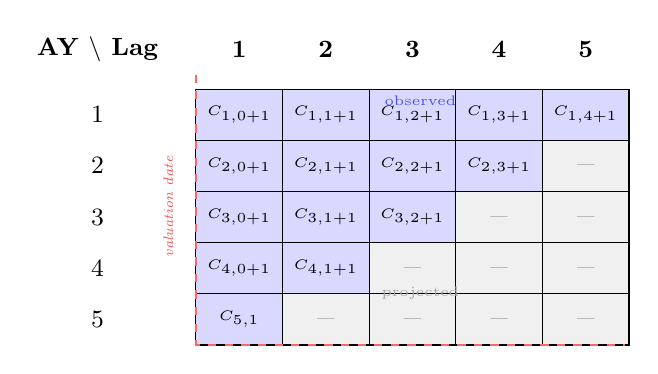
\begin{tikzpicture}[
    cell/.style={draw, minimum width=1.1cm, minimum height=0.65cm,
                 font=\tiny, inner sep=1pt},
    observed/.style={cell, fill=blue!15},
    missing/.style={cell, fill=gray!12, text=gray},
    header/.style={font=\small\bfseries},
    yearlab/.style={font=\small}
  ]

  % Column headers (development lags)
  \foreach \k/\klab in {0/1, 1/2, 2/3, 3/4, 4/5} {
    \node[header] at (1.1*\k + 1.5, 0.5) {\klab};
  }
  \node[header] at (-0.3, 0.5) {AY $\backslash$ Lag};

  % Row labels and cells
  % AY 1 -- 5 observed lags
  \node[yearlab] at (-0.3, -0.33)  {1};
  \foreach \k in {0,...,4} { \node[observed] at (1.1*\k + 1.5, -0.33) {$C_{1,\k+1}$}; }

  % AY 2 -- 4 observed lags
  \node[yearlab] at (-0.3, -0.98)  {2};
  \foreach \k in {0,...,3} { \node[observed] at (1.1*\k + 1.5, -0.98) {$C_{2,\k+1}$}; }
  \node[missing] at (1.1*4 + 1.5, -0.98) {---};

  % AY 3 -- 3 observed lags
  \node[yearlab] at (-0.3, -1.63) {3};
  \foreach \k in {0,...,2} { \node[observed] at (1.1*\k + 1.5, -1.63) {$C_{3,\k+1}$}; }
  \foreach \k in {3,...,4} { \node[missing] at (1.1*\k + 1.5, -1.63) {---}; }

  % AY 4 -- 2 observed lags
  \node[yearlab] at (-0.3, -2.28) {4};
  \foreach \k in {0,...,1} { \node[observed] at (1.1*\k + 1.5, -2.28) {$C_{4,\k+1}$}; }
  \foreach \k in {2,...,4} { \node[missing] at (1.1*\k + 1.5, -2.28) {---}; }

  % AY 5 -- 1 observed lag
  \node[yearlab] at (-0.3, -2.93) {5};
  \node[observed] at (1.5, -2.93) {$C_{5,1}$};
  \foreach \k in {1,...,4} { \node[missing] at (1.1*\k + 1.5, -2.93) {---}; }

  % Diagonal boundary annotation
  \draw[dashed, thick, red!60]
    (0.95, 0.18) -- (0.95, -3.25) -- (6.4, -3.25);

  % Labels
  \node[red!70, font=\tiny\itshape, rotate=90] at (0.6, -1.5) {valuation date};
  \node[blue!70, font=\tiny] at (3.8, -0.15) {observed};
  \node[gray!70, font=\tiny] at (3.8, -2.60) {projected};

\end{tikzpicture}
\caption{Structure of a loss development triangle. Blue cells are observed;
gray cells lie beyond the valuation date and must be projected.
The diagonal boundary represents the valuation date.}
\label{fig:loss-triangle}
\end{figure}

\subsection{From Long Format to Triangle}

The raw CAS data is in \emph{long format} (one row per accident
year $\times$ development lag). The function \texttt{build\_triangle()} in
\filepath{04\_compute\_reserves.py} pivots this into the standard matrix form
using \texttt{pandas.pivot\_table}:

\begin{lstlisting}[style=python, caption={Triangle construction in \texttt{04\_compute\_reserves.py}}]
def build_triangle(df, lob, value_col="IncurLoss"):
    lob_data = df[
        (df["line_of_business"] == lob)
        & (df["DevelopmentYear"] <= VALUATION_YEAR)   # 1997 cutoff
    ].copy()
    pivot = lob_data.pivot_table(
        index="AccidentYear",
        columns="DevelopmentLag",
        values=value_col,
        aggfunc="sum",
    )
    return pivot  # NaN in lower-right = future cells
\end{lstlisting}

The SQL equivalent is in \filepath{sql/04\_triangle\_pivot.sql}, which uses
PostgreSQL's conditional aggregation pattern to pivot lags 1--10 into
separate columns:

\begin{lstlisting}[style=sql, caption={Triangle pivot in SQL (\texttt{04\_triangle\_pivot.sql})}]
SELECT
    line_of_business, accident_year,
    MAX(incur_loss) FILTER (WHERE development_lag = 1) AS incurred_lag_01,
    MAX(incur_loss) FILTER (WHERE development_lag = 2) AS incurred_lag_02,
    -- ... lags 3-10 ...
    ROUND(incurred_lag_02 / NULLIF(incurred_lag_01, 0), 4) AS ata_01_02
FROM triangles
GROUP BY line_of_business, accident_year;
\end{lstlisting}

% -----------------------------------------------------------------------------
\section{Chain-Ladder Method}
\label{sec:ins-chain-ladder}
% -----------------------------------------------------------------------------

\sourcefiles{%
  \filepath{data-pipeline/04\_compute\_reserves.py} (lines 59--135),
  \filepath{backend/insurance\_backend/routers/loss\_triangle.py} (lines 67--93)
}

The \textbf{Chain-Ladder method} (also called the \emph{Development Method})
is the actuarial workhorse for loss reserving.  It assumes that loss
development follows a stable, repeatable pattern captured by historical
age-to-age factors.

\subsection{Age-to-Age Development Factors}

For each transition from development lag $k$ to lag $k+1$, the
\textbf{volume-weighted age-to-age factor} is:

\begin{equation}
  \hat{f}_k = \frac{\displaystyle\sum_{i:\, C_{i,k+1} \text{ observed}}
                      C_{i,k+1}}
                   {\displaystyle\sum_{i:\, C_{i,k+1} \text{ observed}}
                      C_{i,k}}
  \label{eq:ata-factor}
\end{equation}

Volume-weighting (rather than simple averaging) gives larger, more-developed
accident years greater influence -- appropriate because they represent more
statistical credibility.

\paragraph{Code implementation.}
The function \texttt{chain\_ladder()} implements Equation~\eqref{eq:ata-factor}
directly:

\begin{lstlisting}[style=python, caption={Age-to-age factor computation (\texttt{04\_compute\_reserves.py}, lines 70--88)}]
for j in range(n_lags - 1):
    col_curr = dev_lags[j]
    col_next = dev_lags[j + 1]
    numerator = 0.0
    denominator = 0.0
    for year in years:
        val_curr = triangle.loc[year, col_curr]
        val_next = triangle.loc[year, col_next]
        if pd.notna(val_curr) and pd.notna(val_next) and val_curr > 0:
            numerator += val_next
            denominator += val_curr
    factors[f"{col_curr}-{col_next}"] = numerator / denominator
\end{lstlisting}

\subsection{Cumulative Development Factors (CDFs)}

The \textbf{cumulative development factor} (CDF) from lag $k$ to ultimate
is the product of all age-to-age factors from lag $k$ onward:

\begin{equation}
  \widehat{\mathrm{CDF}}_k = \prod_{j=k}^{K-1} \hat{f}_j
  \label{eq:cdf}
\end{equation}

where $K$ is the maximum observed development lag (10 in this project).
A tail factor of 1.0 is implicitly assumed (i.e., no further development
beyond lag 10), which is conservative for short-tail lines but may
underestimate for long-tail lines like Medical Malpractice.

\begin{lstlisting}[style=python, caption={CDF computation (\texttt{04\_compute\_reserves.py}, lines 91--97)}]
factor_values = list(factors.values())
cdfs = {}
for j in range(n_lags):
    cdf = 1.0
    for k in range(j, n_lags - 1):
        cdf *= factor_values[k]
    cdfs[dev_lags[j]] = cdf
\end{lstlisting}

\subsection{Projecting Ultimate Losses}

For accident year $i$ with the latest available observation at lag $k$,
the projected ultimate loss is:

\begin{equation}
  \hat{U}_i = C_{i,k} \times \widehat{\mathrm{CDF}}_k
  \label{eq:ultimate}
\end{equation}

\subsection{IBNR Reserve Estimation}

The \textbf{IBNR reserve} for accident year $i$ is the difference between
projected ultimate and current reported losses:

\begin{equation}
  \widehat{\mathrm{IBNR}}_i = \max\!\left(0,\; \hat{U}_i - C_{i,k}\right)
  \label{eq:ibnr-cl}
\end{equation}

The $\max(0, \cdot)$ floor prevents negative IBNR from arising due to
favorable development (reserve releases).

\paragraph{Numerical example.}
For Private Passenger Auto, paid development factors
(from the \texttt{main()} output) illustrate the method:

\begin{center}
\begin{tabular}{ccc}
\toprule
\textbf{Lag transition} & \textbf{Factor} $\hat{f}_k$
  & \textbf{CDF} $\widehat{\mathrm{CDF}}_k$ \\
\midrule
1 $\to$ 2 & 1.80 & $1.80 \times \cdots$ \\
2 $\to$ 3 & 1.25 & $\cdots$ \\
$\vdots$   & $\vdots$ & $\vdots$ \\
$k \to$ ultimate & 1.00 & 1.00 \\
\bottomrule
\end{tabular}
\end{center}

The 1997 accident year has only lag-1 data available; its CDF is the
product of all nine factors, making the IBNR estimate highly leveraged
on historical patterns -- exactly why BF was developed as a complement.

\begin{keyinsight}
The portfolio's total IBNR on a paid Chain-Ladder basis is approximately
\$20.4M, with Private Passenger Auto contributing 76\% due to its volume.
Medical Malpractice carries paid CDF values of 6.1x at lag 1--2,
meaning that only 1/6.1 $\approx$ 16\% of ultimate losses have been paid
by end of year 2 -- illustrating why long-tail lines require large IBNR reserves.
\end{keyinsight}

% -----------------------------------------------------------------------------
\section{Bornhuetter-Ferguson Method}
\label{sec:ins-bf}
% -----------------------------------------------------------------------------

\sourcefiles{%
  \filepath{data-pipeline/04\_compute\_reserves.py} (lines 138--180),
  \filepath{backend/insurance\_backend/routers/loss\_triangle.py} (lines 122--145)
}

\subsection{Motivation}

The Chain-Ladder method relies entirely on observed data.  For recent
accident years (e.g., 1997, which has only one year of development),
the CL estimate is highly volatile -- a single unusual claim year
extrapolates to a large IBNR.  The \textbf{Bornhuetter-Ferguson method}
(BF) blends CL-derived development patterns with an \emph{a priori}
expected loss ratio, moderating the influence of sparse data.

\subsection{Derivation}

Partition ultimate losses into two components:
\begin{enumerate}
  \item Losses already reported (observed): $C_{i,k}$
  \item Losses yet to emerge (unreported): estimated from an a priori expectation
\end{enumerate}

The fraction of losses \emph{yet to be reported} as of lag $k$ is:
\begin{equation}
  q_k = 1 - \frac{1}{\widehat{\mathrm{CDF}}_k}
  \label{eq:pct-unreported}
\end{equation}

The \textbf{a priori expected loss} for accident year $i$ is:
\begin{equation}
  \mathrm{EL}_i = \mathrm{Premium}_i \times \mathrm{ELR}
  \label{eq:expected-loss}
\end{equation}
where ELR (\emph{expected loss ratio}) is the actuary's a priori assumption
about profitability -- typically derived from pricing actuaries, industry
benchmarks, or long-run historical averages.

The \textbf{BF IBNR} is:
\begin{align}
  \widehat{\mathrm{IBNR}}_i^{\,\mathrm{BF}}
    &= \mathrm{EL}_i \times q_k \notag \\
    &= \mathrm{Premium}_i \times \mathrm{ELR}
       \times \left(1 - \frac{1}{\widehat{\mathrm{CDF}}_k}\right)
  \label{eq:bf-ibnr}
\end{align}

The \textbf{BF ultimate} is the sum of observed losses and BF IBNR:
\begin{equation}
  \hat{U}_i^{\,\mathrm{BF}} = C_{i,k}
    + \mathrm{Premium}_i \times \mathrm{ELR}
      \times \left(1 - \frac{1}{\widehat{\mathrm{CDF}}_k}\right)
  \label{eq:bf-ultimate}
\end{equation}

\subsection{Code Implementation}

The project uses \texttt{apriori\_lr = 0.65} (65\% expected loss ratio),
a reasonable starting assumption for a mixed P\&C portfolio:

\begin{lstlisting}[style=python, caption={Bornhuetter-Ferguson (\texttt{04\_compute\_reserves.py}, lines 159--177)}]
def bornhuetter_ferguson(triangle, earned_premium, cl_cdfs,
                         apriori_lr=0.65):
    for year in sorted(triangle.index):
        latest_lag = available.index.max()
        reported   = float(available[latest_lag])
        cdf        = cl_cdfs.get(latest_lag, 1.0)
        prem       = earned_premium.get(year, 0)
        expected_loss = prem * apriori_lr

        pct_unreported = max(0, 1 - 1/cdf) if cdf > 1 else 0
        ibnr_bf        = expected_loss * pct_unreported
        ultimate_bf    = reported + ibnr_bf
\end{lstlisting}

\subsection{CL vs.\ BF Comparison}

\begin{center}
\begin{tabular}{p{4cm} p{5cm} p{5cm}}
\toprule
\textbf{Criterion} & \textbf{Chain-Ladder} & \textbf{Bornhuetter-Ferguson} \\
\midrule
Data requirement
  & Development pattern only
  & Pattern + a priori loss ratio \\
Mature years (early lags)
  & Accurate; data-rich
  & Converges to CL as $q_k \to 0$ \\
Immature years (late AYs)
  & Volatile; highly leveraged
  & Moderate; a priori anchors estimate \\
Regulatory preference
  & Standard; widely accepted
  & Often preferred for most-recent years \\
Sensitivity to one bad year
  & High (contaminates all factors)
  & Low (a priori is independent) \\
When to use
  & Long-run stable portfolios with credible history
  & New books of business; recent AYs; volatile LOBs \\
\bottomrule
\end{tabular}
\end{center}

\begin{keyinsight}
CL produces larger IBNR estimates for the most recent accident years
(1996--1997) where little development data is available; BF moderates these
projections toward the a priori expectation.  This difference is visible in
the \texttt{/api/v1/cl-vs-bf} endpoint, which returns \texttt{pct\_diff}
(the percentage by which BF IBNR differs from CL IBNR) for each accident year
and LOB.
\end{keyinsight}

% -----------------------------------------------------------------------------
\section{Profitability Analysis}
\label{sec:ins-profitability}
% -----------------------------------------------------------------------------

\sourcefiles{%
  \filepath{sql/02\_loss\_ratio\_by\_lob.sql},
  \filepath{sql/03\_frequency\_severity.sql},
  \filepath{sql/05\_combined\_ratio.sql},
  \filepath{data-pipeline/04\_compute\_reserves.py} (lines 288--294)
}

\subsection{Loss Ratio}

The \textbf{loss ratio} is the primary underwriting profitability metric:

\begin{equation}
  \mathrm{LR}_i = \frac{\text{Incurred Losses}_i}{\text{Earned Premium}_i}
  \label{eq:loss-ratio}
\end{equation}

An LR below 100\% means the line collected more premium than it paid in
losses (before expenses).  The SQL in \filepath{02\_loss\_ratio\_by\_lob.sql}
computes both a reported LR and an ultimate LR (using CL projections):

\begin{lstlisting}[style=sql, caption={Loss ratio computation (\texttt{02\_loss\_ratio\_by\_lob.sql})}]
annual_loss_ratio AS (
    SELECT
        line_of_business, accident_year,
        ROUND(100.0 * incur_loss
              / NULLIF(earned_prem_net, 0), 2) AS loss_ratio_pct,
        -- Rolling 3-year average to smooth volatility
        ROUND(AVG(loss_ratio_pct) OVER (
            PARTITION BY line_of_business
            ORDER BY accident_year
            ROWS BETWEEN 2 PRECEDING AND CURRENT ROW
        ), 2)                                  AS rolling_3yr_lr_pct
    FROM latest_eval
)
\end{lstlisting}

Profitability flags are assigned: \texttt{PROFITABLE} ($< 100\%$),
\texttt{MARGINAL} (90--100\%), \texttt{UNPROFITABLE} ($> 100\%$).

\subsection{Combined Ratio}

The \textbf{combined ratio} is the gold-standard underwriting metric,
incorporating both claim costs and operational expenses:

\begin{equation}
  \mathrm{CR} = \mathrm{LR} + \mathrm{ER}
  = \frac{\text{Incurred Losses} + \text{Expenses}}{\text{Earned Premium}}
  \label{eq:combined-ratio}
\end{equation}

where ER is the expense ratio.  A CR below 100\% means underwriting profit;
above 100\% means the insurer relies on investment income to be profitable.

\begin{center}
\begin{tabular}{ll}
\toprule
\textbf{Combined Ratio} & \textbf{Interpretation} \\
\midrule
$< 95\%$   & Strong underwriting profit \\
$95-100\%$ & Marginal profit \\
$100-110\%$ & Marginal loss; investment income may compensate \\
$> 110\%$  & Significant loss \\
\bottomrule
\end{tabular}
\end{center}

The project assumes a flat 30\% expense ratio (U.S. industry average for P\&C):
\begin{equation}
  \mathrm{CR} = \mathrm{LR} + 0.30
  \label{eq:combined-ratio-assumed}
\end{equation}

This assumption is made explicit in the SQL via a \texttt{params} CTE
to facilitate sensitivity analysis.

\subsection{Frequency-Severity Decomposition}

The fundamental identity of insurance pricing:

\begin{equation}
  \text{Pure Premium} = \text{Frequency} \times \text{Severity}
  \label{eq:pure-premium}
\end{equation}

where:
\begin{align}
  \text{Frequency} &= \frac{\text{Claim Count}}{\text{Exposure}}
  \label{eq:frequency} \\
  \text{Severity}  &= \frac{\text{Total Losses}}{\text{Claim Count}}
  \label{eq:severity}
\end{align}

This decomposition is critical for claims management decisions:
rising frequency signals underwriting/risk selection problems;
rising severity signals claims management or trend issues.

The SQL in \filepath{03\_frequency\_severity.sql} computes year-over-year
growth rates for both components and flags the \emph{primary loss driver}:

\begin{lstlisting}[style=sql, caption={Loss driver identification (\texttt{03\_frequency\_severity.sql})}]
CASE
    WHEN ABS(frequency_yoy_pct) > ABS(severity_yoy_pct)
        THEN 'FREQUENCY DRIVEN'
    WHEN ABS(severity_yoy_pct) > ABS(frequency_yoy_pct)
        THEN 'SEVERITY DRIVEN'
    ELSE 'BALANCED'
END AS primary_loss_driver
\end{lstlisting}

Since the project uses synthetic claims, exposure is proxied by earned premium,
yielding a \emph{pure premium rate} (loss per dollar of premium) rather than
traditional frequency per policy.

\begin{keyinsight}
From the README findings:
\textbf{Private Passenger Auto} and \textbf{Product Liability} are the only
profitable lines (combined ratio $< 100\%$).  \textbf{Medical Malpractice}
shows the highest loss ratio ($\approx 280\%$) with the longest development
tails -- claims take 3--5$\times$ longer to report than Auto, creating the
largest IBNR uncertainty of all six LOBs.
\end{keyinsight}

% -----------------------------------------------------------------------------
\section{System Architecture}
\label{sec:ins-architecture}
% -----------------------------------------------------------------------------

\sourcefiles{%
  \filepath{backend/insurance\_backend/main.py},
  \filepath{backend/insurance\_backend/data\_loader.py},
  \filepath{src/components/insurance/InsuranceDashboard.tsx}
}

\subsection{4-Stage ETL Pipeline}

\begin{center}
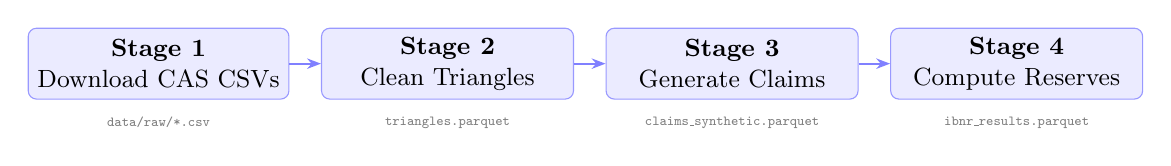
\begin{tikzpicture}[
    node distance=0.4cm,
    box/.style={draw, rounded corners=3pt, minimum width=3.2cm,
                minimum height=0.9cm, align=center, font=\small,
                fill=blue!8, draw=blue!40},
    arrow/.style={-{Stealth[length=5pt]}, thick, blue!50}
  ]

  \node[box] (s1) {\textbf{Stage 1}\\Download CAS CSVs};
  \node[box, right=of s1] (s2) {\textbf{Stage 2}\\Clean Triangles};
  \node[box, right=of s2] (s3) {\textbf{Stage 3}\\Generate Claims};
  \node[box, right=of s3] (s4) {\textbf{Stage 4}\\Compute Reserves};

  \draw[arrow] (s1) -- (s2);
  \draw[arrow] (s2) -- (s3);
  \draw[arrow] (s3) -- (s4);

  % Output labels
  \node[font=\tiny, gray, below=0.1cm of s1] {\texttt{data/raw/*.csv}};
  \node[font=\tiny, gray, below=0.1cm of s2] {\texttt{triangles.parquet}};
  \node[font=\tiny, gray, below=0.1cm of s3] {\texttt{claims\_synthetic.parquet}};
  \node[font=\tiny, gray, below=0.1cm of s4] {\texttt{ibnr\_results.parquet}};

\end{tikzpicture}
\end{center}

\begin{description}
  \item[Stage 1 -- \filepath{01\_download\_cas.py}]
    Downloads six CAS CSVs from \texttt{casact.org}.  Idempotent: skips files
    that already exist.

  \item[Stage 2 -- \filepath{02\_clean\_triangles.py}]
    Detects and strips per-file column suffixes, tags each row with a
    human-readable LOB name, selects top 5 companies per LOB by premium volume,
    and computes derived columns (\texttt{loss\_ratio},
    \texttt{paid\_to\_incurred}).
    Output: \filepath{data/processed/triangles.parquet}.

  \item[Stage 3 -- \filepath{03\_generate\_claims.py}]
    Generates 50,000 synthetic claims using LOB-calibrated lognormal severity,
    exponential report lag, and gamma settlement distributions.
    Output: \filepath{data/processed/claims\_synthetic.parquet}.

  \item[Stage 4 -- \filepath{04\_compute\_reserves.py}]
    Builds valuation-date triangles for both incurred and paid bases, runs
    chain-ladder on each, runs BF on paid losses with \texttt{apriori\_lr = 0.65},
    and aggregates LOB-level summaries.
    Outputs: \filepath{data/processed/ibnr\_results.parquet} and
    \filepath{data/processed/lob\_summary.parquet}.
\end{description}

\subsection{FastAPI Backend}

The backend loads all four parquet files at startup via
\filepath{backend/insurance\_backend/data\_loader.py} and exposes five API
routers under the \texttt{/api/v1} prefix:

\begin{center}
\begin{tabular}{ll}
\toprule
\textbf{Router module} & \textbf{Endpoint} \\
\midrule
\texttt{loss\_triangle.py}        & \texttt{GET /api/v1/loss-triangle} \\
                                  & \texttt{GET /api/v1/cl-vs-bf} \\
\texttt{frequency\_severity.py}   & \texttt{GET /api/v1/frequency-severity} \\
\texttt{loss\_ratios.py}          & \texttt{GET /api/v1/loss-ratios} \\
\texttt{combined\_ratio.py}       & \texttt{GET /api/v1/combined-ratio} \\
\texttt{claim\_distribution.py}   & \texttt{GET /api/v1/claim-distribution} \\
\bottomrule
\end{tabular}
\end{center}

All endpoints accept optional query parameters \texttt{lob}, \texttt{company},
\texttt{year\_start}, and \texttt{year\_end} for dashboard filtering.
The \texttt{/api/v1/loss-triangle} endpoint additionally accepts
\texttt{type} (\texttt{incurred}/\texttt{paid}) and \texttt{method}
(\texttt{cl}/\texttt{bf}), computing CL factors on-the-fly from the filtered
triangle and overriding the IBNR estimates from the pre-computed parquet when
BF is requested.

\subsection{Next.js Frontend}

The dashboard runs at \texttt{localhost:3051} and proxies all API calls through
Next.js rewrites to avoid CORS issues.  Browser traffic never reaches the
FastAPI port directly.

Key React components in
\filepath{src/components/insurance/}:

\begin{itemize}
  \item \texttt{LossTriangleHeatmap.tsx} -- interactive heatmap; toggle
    incurred/paid and CL/BF
  \item \texttt{IBNRWaterfall.tsx} -- waterfall: Paid + Case Reserve + IBNR = Ultimate
  \item \texttt{FrequencySeverityChart.tsx} -- dual-axis: claim count (bars)
    and avg severity (line)
  \item \texttt{LossRatioByLOB.tsx} -- reported vs.\ ultimate LR bar chart
  \item \texttt{CombinedRatioTrend.tsx} -- stacked area: loss ratio + expense ratio
  \item \texttt{CLvsBFTable.tsx} -- tabular comparison of CL and BF IBNR by year
  \item \texttt{InsuranceFilterBar.tsx} -- LOB / company / year-range selectors
\end{itemize}

\begin{decisionbox}
\textbf{Why Next.js instead of Power BI?}
Power BI was the original plan, but it requires a Windows machine with PBI
Desktop and a licensed workspace for embedding.  Next.js + Recharts gives
full control over dark/light theming (the dashboard supports both modes with
LOB-specific CSS variables like \texttt{--lob-auto}, \texttt{--lob-workers}),
a static export that merges into the shared portfolio hub, and the ability to
call FastAPI endpoints through an edge proxy rather than exposing them.  The actuarial calculations remain in Python,
which is far more transparent than DAX measures.
\end{decisionbox}

% -----------------------------------------------------------------------------
\section{SQL Queries}
\label{sec:ins-sql}
% -----------------------------------------------------------------------------

\sourcefiles{%
  \filepath{sql/01\_claims\_summary.sql},
  \filepath{sql/02\_loss\_ratio\_by\_lob.sql},
  \filepath{sql/03\_frequency\_severity.sql},
  \filepath{sql/04\_triangle\_pivot.sql},
  \filepath{sql/05\_combined\_ratio.sql}
}

Five analytical SQL queries cover the full story from raw claims to
underwriting decision support.  All are written in PostgreSQL dialect with
CTEs for readability.

\paragraph{Query 01 -- Claims portfolio snapshot.}
\emph{Business question: What does our claims landscape look like by LOB and status?}

Produces count, open/closed split, average severity (paid and incurred),
total case reserves, and severity-band distribution per LOB.
Uses three CTEs: \texttt{claims\_by\_lob\_status} $\to$
\texttt{lob\_pivot} (conditional sums for open/closed) $\to$
\texttt{portfolio\_totals} (UNION ALL grand total row).
Key pattern: \texttt{NULLIF(denominator, 0)} guards every division.

\paragraph{Query 02 -- Loss ratio by LOB.}
\emph{Business question: Which lines of business are profitable?}

Joins triangles (most mature lag per accident year via \texttt{DISTINCT ON})
to \texttt{ibnr\_results} for ultimate loss ratios.  Adds a rolling 3-year
window average:

\begin{lstlisting}[style=sql, caption={Rolling window loss ratio (\texttt{02\_loss\_ratio\_by\_lob.sql})}]
AVG(loss_ratio_pct) OVER (
    PARTITION BY line_of_business
    ORDER BY accident_year
    ROWS BETWEEN 2 PRECEDING AND CURRENT ROW
) AS rolling_3yr_lr_pct
\end{lstlisting}

Assigns \texttt{CHRONIC ISSUE} when the rolling 3-year average exceeds 100\%,
directing management attention to persistently unprofitable lines.

\paragraph{Query 03 -- Frequency-severity decomposition.}
\emph{Business question: Are losses driven by more claims or larger claims?}

Joins \texttt{claims\_synthetic} to \texttt{triangles} for an exposure proxy,
computes frequency per \$1M of earned premium and incurred severity, then
uses \texttt{LAG()} window functions to produce year-over-year growth rates.
The \texttt{primary\_loss\_driver} flag guides management action:
frequency-driven losses suggest underwriting intervention; severity-driven
losses suggest claims management improvements.

\paragraph{Query 04 -- Triangle pivot.}
\emph{Business question: What does the loss development pattern look like?}

Pivots the long-format triangles table into the standard actuarial wide
layout using \texttt{FILTER (WHERE development\_lag = k)} conditional
aggregation.  Also computes individual age-to-age factors per accident year
and volume-weighted average factors in a separate CTE -- the equivalent of
what the Python chain-ladder code does, but expressible in pure SQL.

\paragraph{Query 05 -- Combined ratio analysis.}
\emph{Business question: Is the portfolio profitable after expenses?}

Uses a \texttt{params} CTE (\texttt{assumed\_expense\_ratio = 0.30}) to
make the flat expense assumption explicit and easy to change.  Computes
reported CR, ultimate CR (including IBNR from chain-ladder), a 3-year rolling
CR, and year-over-year CR change.  Profitability bands (\texttt{STRONG PROFIT}
through \texttt{SIGNIFICANT LOSS}) and trend flags (\texttt{IMPROVING},
\texttt{DETERIORATING}, \texttt{STABLE}) provide dashboard-ready text labels.

% -----------------------------------------------------------------------------
\section{Challenge and Interview Questions}
\label{sec:ins-questions}
% -----------------------------------------------------------------------------

\begin{challengebox}
\textbf{Triangle completeness and the valuation date.}
The code sets \texttt{VALUATION\_YEAR = 1997}.  If you moved the valuation
date to 1993, which cells in the triangle would be removed?  How would the
chain-ladder factors change, and in which direction would IBNR estimates
move for the 1993 accident year?  Explain using Equation~\eqref{eq:ata-factor}.
\end{challengebox}

\begin{challengebox}
\textbf{Tail factor sensitivity.}
The project assumes a tail factor of 1.000 beyond lag 10 for all LOBs.
For Medical Malpractice (a very long-tail line), this is arguably wrong.
If you applied a tail factor of 1.15 (15\% additional development beyond lag 10),
how would the IBNR change for the oldest accident year (1988)?  Show the
algebraic adjustment to Equations~\eqref{eq:cdf} and \eqref{eq:ultimate}.
\end{challengebox}

\begin{challengebox}
\textbf{BF convergence.}
Prove algebraically that as $k \to K$ (i.e., as an accident year approaches
full development), the BF ultimate in Equation~\eqref{eq:bf-ultimate}
converges to the observed value $C_{i,K}$.  What does this imply about when
BF and CL agree?
\end{challengebox}

\begin{challengebox}
\textbf{Volume weighting vs.\ simple average.}
The code computes volume-weighted factors (Equation~\eqref{eq:ata-factor}).
Construct a numerical example with three accident years where the simple-average
factor and the volume-weighted factor differ by more than 10\%.  Which is
more appropriate and why?  When might an actuary deliberately choose a simple
average or an ``all-but-one-year'' factor selection?
\end{challengebox}

\begin{interviewbox}
\textbf{Explain IBNR to a non-actuarial CFO.}
The CFO asks: ``Our loss triangle shows \$15M of paid losses.  Your report
says our ultimate is \$20.4M.  Where did the extra \$5.4M come from, and
do we actually owe it?''  Give a 2-minute plain-language answer.
\end{interviewbox}

\begin{interviewbox}
\textbf{When would you choose BF over Chain-Ladder?}
The pricing team just launched a new commercial auto product six months ago.
You have half a year of loss data.  Which method would you use to estimate
IBNR and why?  What a priori loss ratio would you select, and where does
it come from?
\end{interviewbox}

\begin{interviewbox}
\textbf{Combined ratio interpretation.}
Medical Malpractice shows a combined ratio of approximately 310\% in this
project.  Does that mean the insurer is bankrupt?  What information would
you need to determine whether the company is financially viable despite
this underwriting loss?
\end{interviewbox}

\begin{interviewbox}
\textbf{Frequency-severity trade-offs in pricing.}
Your analysis flags a line as ``SEVERITY DRIVEN'' because average incurred
severity increased 12\% year-over-year while frequency was flat.  What are
three possible root causes of rising severity?  For each, describe the
management response that would be appropriate.
\end{interviewbox}

% =============================================================================
% CHAPTER 02 -- E-Commerce Cohort Analysis (Olist)
% =============================================================================

\chapter{E-Commerce Cohort Analysis}
\label{ch:ecommerce}

\sourcefiles{%
  \filepath{projects/02-ecommerce-cohort-analysis/} ---
  notebooks (4), SQL scripts (5), Streamlit app (6 pages)
}

This chapter documents the analytical work behind the Olist Brazilian E-Commerce
cohort analysis. The central business question is deceptively simple: with only
3\% of customers making a repeat purchase, what distinguishes the returning
minority? The project delivers statistical rigour --- survival curves, odds ratios,
Gini coefficients --- through a multi-layer stack of SQL, Python notebooks, and a
Streamlit executive dashboard deployed to Cloud Run.

% -----------------------------------------------------------------------------
\section{Business Context}
\label{sec:ecom-context}
% -----------------------------------------------------------------------------

\subsection{The 3\% Repeat Purchase Problem}

Olist is a Brazilian marketplace intermediary: sellers list products on Olist's
platform and Olist handles the customer-facing experience. The dataset covers
99,441 orders placed between September 2016 and October 2018. Of 93,358 unique
customers, only 2,801 --- roughly 3.0\% --- ever placed a second delivered order.

This figure is the analytical anchor of the entire project. It frames every
downstream analysis as a search for signal within extreme class imbalance.
Repeat customers are worth \textbf{1.92x} a one-time customer in \emph{total}
revenue (R\$309 against R\$161), but the reason is order count, not basket size:
they place roughly 2.1 orders. \emph{Per order} they spend \textbf{0.91x} as much
(R\$146 against R\$161), and their first order is about 10\% smaller than a
one-and-done customer's. The high spenders are disproportionately the ones who
never come back, which inverts the naive reading --- retention is valuable
because of frequency, not because returning customers are richer.

\begin{keyinsight}
A 3\% base rate means that standard accuracy metrics are meaningless for
classification tasks. Any model predicting ``never repeat'' would achieve 97\%
accuracy while being analytically useless. The project therefore avoids binary
classification in favour of survival analysis (which respects censoring) and
logistic regression odds ratios (which quantify relative risk between groups).
\end{keyinsight}

\subsection{The \texttt{customer\_id} vs.\ \texttt{customer\_unique\_id} Distinction}

Olist's schema contains two customer identifiers that are easily confused:

\begin{itemize}
  \item \texttt{customer\_id}: generated per order. A single person placing three
    orders will have three distinct \texttt{customer\_id} values.
  \item \texttt{customer\_unique\_id}: the true person-level identifier, stable
    across all orders.
\end{itemize}

Using \texttt{customer\_id} directly would cause three critical errors: (1) it
would inflate the apparent customer count, (2) every order would appear as a
first purchase, and (3) the repeat rate would compute to zero by construction.
All SQL scripts and Python code in this project join through
\texttt{customer\_id} only to resolve the link to \texttt{customer\_unique\_id},
then group exclusively on the latter.

\begin{lstlisting}[style=sql, caption={Wrong vs.\ correct customer grouping}]
-- WRONG: one row per order, not per person
SELECT customer_id, COUNT(*) AS orders
FROM olist_orders
GROUP BY customer_id;

-- CORRECT: one row per real customer
SELECT c.customer_unique_id, COUNT(*) AS orders
FROM olist_orders  o
JOIN olist_customers c ON o.customer_id = c.customer_id
GROUP BY c.customer_unique_id;
\end{lstlisting}

\subsection{Olist Marketplace Model}

Because Olist is an intermediary, the customer experience depends on three
parties: Olist (platform, review system, logistics coordination), the individual
seller (product quality, dispatch time), and the carrier. This creates a
confounding structure for causal claims: a poor delivery experience may reflect
the seller, the carrier, or geographic distance --- not Olist platform quality
per se. The analysis treats delivery days and review scores as observed outcomes
without attributing causality to any single party.

% -----------------------------------------------------------------------------
\section{Olist Dataset}
\label{sec:ecom-data}
% -----------------------------------------------------------------------------

\sourcefiles{%
  \filepath{streamlit/pages/5\_metodologia.py} (tab ``Fuente de Datos''),
  \filepath{notebooks/01\_data\_ingestion\_cleaning.ipynb}
}

\subsection{Nine CSV Files, One Analytical Table}

The raw dataset consists of nine CSV files joined into a single master table
(\filepath{data/processed/orders\_enriched.parquet}) during notebook 01. The
join graph is star-shaped: \texttt{olist\_orders} is the central fact table,
with dimension tables for customers, items, payments, reviews, products, sellers,
geolocation, and a category translation lookup.

\begin{table}[h]
\centering
\caption{Olist dataset files and approximate row counts}
\label{tab:olist-files}
\begin{tabular}{llr}
\toprule
\textbf{CSV file} & \textbf{Content} & \textbf{Rows (approx.)} \\
\midrule
\texttt{olist\_orders\_dataset.csv}         & Orders: status, timestamps, customer\_id & 99,441 \\
\texttt{olist\_order\_items\_dataset.csv}   & Line items: price, freight, seller       & 112,650 \\
\texttt{olist\_customers\_dataset.csv}      & customer\_id $\to$ unique\_id, state     & 99,441 \\
\texttt{olist\_products\_dataset.csv}       & Category, dimensions, weight             & 32,951 \\
\texttt{olist\_sellers\_dataset.csv}        & Seller state and city                    & 3,095 \\
\texttt{olist\_order\_payments\_dataset.csv}& Payment type, value, instalments         & 103,886 \\
\texttt{olist\_order\_reviews\_dataset.csv} & Review score 1--5, free text             & 100,000 \\
\texttt{olist\_geolocation\_dataset.csv}    & ZIP $\to$ lat/lon                        & 1,000,163 \\
\texttt{product\_category\_name\_translation.csv} & Portuguese $\to$ English category  & 71 \\
\bottomrule
\end{tabular}
\end{table}

The enriched parquet adds 30 derived columns including \texttt{delivery\_days},
\texttt{is\_late\_delivery}, \texttt{cohort\_month}, \texttt{months\_since\_cohort},
and aggregated payment totals. The analysis filters to 96,478 delivered orders
only; cancelled, unavailable, and invoiced orders are excluded because their
customer journey is incomplete.

\subsection{Right-Censoring Problem}

The observation window closes at October 2018. Any customer who made their first
purchase in, say, August 2018 has had at most two months to return. We cannot
observe whether they return in November 2018 or later. This is right-censoring
in the survival analysis sense: the event (second purchase) may have happened
after the observation period ended.

\begin{decisionbox}
Three approaches were considered for handling censoring:
\begin{enumerate}
  \item \textbf{Ignore it}: count non-repeaters as definitive churners. This
    underestimates the true repeat rate for recent cohorts.
  \item \textbf{Truncate}: only analyse cohorts old enough to have a full 12-month
    window. This wastes 40\%+ of the data and introduces selection bias toward early cohorts.
  \item \textbf{Kaplan-Meier} (chosen): treat non-repeaters as right-censored
    observations. This correctly accounts for the fact that recent customers have
    had less time to return, without discarding them.
\end{enumerate}
The Kaplan-Meier approach is implemented via the \texttt{lifelines} library.
The \texttt{event\_observed} column is 1 for confirmed repeaters and 0 for
right-censored customers.
\end{decisionbox}

% -----------------------------------------------------------------------------
\section{Cohort Retention}
\label{sec:ecom-cohorts}
% -----------------------------------------------------------------------------

\sourcefiles{%
  \filepath{sql/01\_cohort\_assignment.sql},
  \filepath{sql/02\_retention\_matrix.sql},
  \filepath{notebooks/03\_cohort\_retention.ipynb},
  \filepath{streamlit/pages/2\_retencion\_cohortes.py}
}

\subsection{Cohort Assignment Logic}

A cohort is defined by the month of a customer's first \emph{delivered} order.
The SQL implementation uses two CTEs: \texttt{customer\_first\_purchase} computes
the minimum \texttt{order\_purchase\_timestamp} per \texttt{customer\_unique\_id},
and \texttt{cohort\_assignment} computes \texttt{months\_since\_cohort} for every
subsequent order.

\begin{lstlisting}[style=sql, caption={Cohort assignment and tenure calculation (from \filepath{sql/01\_cohort\_assignment.sql})}]
customer_first_purchase AS (
    SELECT customer_unique_id,
           MIN(order_purchase_timestamp) AS first_purchase_date
    FROM delivered_orders
    GROUP BY customer_unique_id
),
cohort_assignment AS (
    SELECT d.customer_unique_id,
           DATE_TRUNC('month', fp.first_purchase_date) AS cohort_month,
           (EXTRACT(YEAR FROM AGE(
               DATE_TRUNC('month', d.order_purchase_timestamp),
               DATE_TRUNC('month', fp.first_purchase_date)
           )) * 12
           + EXTRACT(MONTH FROM AGE(
               DATE_TRUNC('month', d.order_purchase_timestamp),
               DATE_TRUNC('month', fp.first_purchase_date)
           )))::INT AS months_since_cohort
    FROM delivered_orders AS d
    JOIN customer_first_purchase AS fp
      ON d.customer_unique_id = fp.customer_unique_id
)
\end{lstlisting}

Note that \texttt{DATE\_TRUNC} is applied before \texttt{AGE} to ensure tenure
is measured in whole months, not fractional months. The final \texttt{SELECT}
also adds \texttt{ROW\_NUMBER() OVER (PARTITION BY customer\_unique\_id ORDER BY
order\_purchase\_timestamp)} to assign a sequential order number, which is used
downstream to isolate first orders in the activation analysis.

\subsection{Retention Matrix Construction}

The retention matrix pivots cohort-month pairs into a wide format using
\texttt{CASE-WHEN} expressions. Each cell reports the percentage of the cohort's
customers who placed a delivered order in that period:

\begin{equation}
\text{Retention}_{c,k} = \frac{\left|\{u \in C_c : \text{purchase in month } k\}\right|}{|C_c|}
\label{eq:retention}
\end{equation}

where $C_c$ is the set of customers in cohort $c$ and $k$ is the number of months
since cohort formation. By construction, $\text{Retention}_{c,0} = 100\%$ for
all cohorts.

\begin{lstlisting}[style=sql, caption={Retention matrix pivot (excerpt from \filepath{sql/02\_retention\_matrix.sql})}]
SELECT
    s.cohort_month,
    s.cohort_size,
    ROUND(MAX(CASE WHEN m.months_since_cohort = 0
        THEN m.active_customers * 100.0 / s.cohort_size END), 2) AS month_0,
    ROUND(MAX(CASE WHEN m.months_since_cohort = 1
        THEN m.active_customers * 100.0 / s.cohort_size END), 2) AS month_1,
    ROUND(MAX(CASE WHEN m.months_since_cohort = 2
        THEN m.active_customers * 100.0 / s.cohort_size END), 2) AS month_2
    -- ... through month_11
FROM cohort_sizes AS s
LEFT JOIN monthly_activity AS m ON s.cohort_month = m.cohort_month
GROUP BY s.cohort_month, s.cohort_size
ORDER BY s.cohort_month;
\end{lstlisting}

\subsection{Count-Based vs.\ Revenue-Based Retention}

The Streamlit dashboard (page 2) offers a toggle between two retention modes:

\begin{itemize}
  \item \textbf{Count-based}: the number of distinct customers active in month $k$
    divided by cohort size. Stored in \filepath{data/processed/cohort\_retention\_matrix.parquet}.
  \item \textbf{Revenue-based}: the total payment value from returning customers in
    month $k$ divided by month-0 revenue. Stored in
    \filepath{data/processed/cohort\_revenue\_retention.parquet}.
\end{itemize}

Revenue retention amplifies the signal of high-value returners. A cohort where
one high-spend customer returns could show high revenue retention but low count
retention. The divergence between the two modes is itself informative: large
gaps suggest that repeat purchases are concentrated among a few high-value
customers rather than broadly distributed.

The Streamlit code normalises both matrices identically:
\begin{lstlisting}[style=python, caption={Normalisation to retention percentages (\filepath{streamlit/pages/2\_retencion\_cohortes.py}, line~90)}]
data_pct = data.div(data.iloc[:, 0], axis=0) * 100
\end{lstlisting}

% -----------------------------------------------------------------------------
\section{Kaplan-Meier Survival Analysis}
\label{sec:ecom-km}
% -----------------------------------------------------------------------------

\sourcefiles{%
  \filepath{notebooks/03\_cohort\_retention.ipynb},
  \filepath{streamlit/pages/2\_retencion\_cohortes.py} (tab ``Kaplan-Meier''),
  \filepath{streamlit/pages/5\_metodologia.py} (tab ``Supervivencia Kaplan-Meier'')
}

\subsection{Estimator Definition}

The Kaplan-Meier (KM) estimator computes the probability that the event of
interest --- here, a second purchase --- has \emph{not} yet occurred by time $t$.
In this project, $S(t)$ is the probability that a customer has not returned
within $t$ days of their first purchase:

\begin{equation}
\hat{S}(t) = \prod_{t_i \leq t} \left(1 - \frac{d_i}{n_i}\right)
\label{eq:km}
\end{equation}

where:
\begin{itemize}
  \item $t_i$ are the ordered distinct event times (days when second purchases occurred),
  \item $d_i$ is the number of second purchases at time $t_i$ (``deaths''),
  \item $n_i$ is the number of customers still at risk at time $t_i$ (neither
    purchased again nor censored before $t_i$).
\end{itemize}

\subsection{Preparing the Survival Dataset}

The \texttt{survival\_data.parquet} file contains one row per customer with two
key columns:

\begin{lstlisting}[style=python, caption={Survival data construction (from \filepath{streamlit/pages/5\_metodologia.py})}]
survival["duration_days"] = np.where(
    survival["is_repeat_customer"],
    (survival["second_purchase_date"] - survival["first_purchase_date"]).dt.days,
    (DATASET_END_DATE - survival["first_purchase_date"]).dt.days,
)
survival["event_observed"] = survival["is_repeat_customer"].astype(int)
\end{lstlisting}

For the 97\% of customers who never returned, \texttt{event\_observed = 0}
and \texttt{duration\_days} measures how long we watched them without seeing a
repeat purchase --- the censoring time, not the time-to-event.

\subsection{Fitting the Model in Streamlit}

The dashboard fits a \texttt{KaplanMeierFitter} from the \texttt{lifelines}
library (version \texttt{>=0.29}) interactively:

\begin{lstlisting}[style=python, caption={KM fitting, originally in \filepath{streamlit/pages/2\_retencion\_cohortes.py}; now precomputed by \filepath{data-pipeline/05\_build\_web\_json.py}}]
from lifelines import KaplanMeierFitter

kmf = KaplanMeierFitter()
kmf.fit(
    durations=survival_clean["duration_days"],
    event_observed=survival_clean["event_observed"],
)
km_df = kmf.survival_function_.reset_index()
ci = kmf.confidence_interval_survival_function_.reset_index()
median_surv = kmf.median_survival_time_   # returns inf: S(t) never reaches 0.5
\end{lstlisting}

\begin{keyinsight}
That last line is a trap worth naming. \texttt{median\_survival\_time\_} returns
\texttt{inf} on this dataset, because $\hat{S}(t)$ plateaus near 0.95 and never
crosses 0.5. Printing it as ``the median'' produces a headline figure that does
not exist. The quotable statistic is conditional on returning, and has to be
computed separately over the uncensored rows.
\end{keyinsight}

The dashboard also supports segmented KM curves: the user selects
\texttt{payment\_type} or \texttt{customer\_state} as a stratification variable,
and the page fits a separate KM curve per group. This directly supports the
log-rank test finding that voucher payers have statistically different survival
curves from credit card and boleto payers.

\subsection{Interpreting the Curve in Context}

For Olist, $\hat{S}(t)$ starts at 1.0 (all customers are ``surviving'' ---
i.e., have not yet reordered) and decays slowly, plateauing near 0.95. The decay
\emph{decelerates but never stops}: the curve loses 1.23 percentage points in the
first quarter and roughly 0.6 points in every quarter thereafter, out to two
years.

\begin{keyinsight}
This corrects an earlier reading of this same dataset, which described reorder
probability as ``practically nil'' after six months. The curve does not support
that. Repurchase keeps trickling in for the full two-year observation window; it
merely slows. The distinction matters for the recommendation, because a
six-month cutoff would write off customers who are still converting.
\end{keyinsight}

Because $\hat{S}(t)$ never crosses 0.5, \textbf{the median survival time does not
exist} --- it is undefined, not merely uninterpretable. What can be quoted is a
conditional statistic: among the 3\% who \emph{did} return, the median wait was
\textbf{82 days}. That is a different quantity and must be labelled as such.

\begin{keyinsight}
The KM curve shows where the density is, not where the opportunity ends. Among
customers who returned, the median wait was 82 days and 27\% came back within
30 --- so the first quarter is the right place to concentrate an intervention.
But since the curve keeps declining for two years, a later touch is not wasted
effort, and framing day 90 as a cutoff would be a misreading of the same data
that motivates the campaign.
\end{keyinsight}

% -----------------------------------------------------------------------------
\section{RFM Segmentation}
\label{sec:ecom-rfm}
% -----------------------------------------------------------------------------

\sourcefiles{%
  \filepath{sql/03\_rfm\_segmentation.sql},
  \filepath{notebooks/04\_rfm\_ltv\_activation.ipynb},
  \filepath{streamlit/pages/3\_segmentos\_clientes.py} (tabs ``Distribucion'' through ``Lorenz'')
}

\subsection{RFM Dimensions and Quintile Scoring}

RFM scores every customer on three behavioural dimensions relative to the
analysis reference date (one day after the last observed purchase):

\begin{table}[h]
\centering
\caption{RFM dimension definitions and scoring direction}
\label{tab:rfm-dims}
\begin{tabular}{llll}
\toprule
\textbf{Dimension} & \textbf{Metric} & \textbf{Direction} & \textbf{Score 5 means} \\
\midrule
Recency (R)   & Days since last purchase  & Lower is better  & Most recent 20\%  \\
Frequency (F) & Count of distinct orders  & Higher is better & Top 20\% by orders \\
Monetary (M)  & Total lifetime spend (R\$) & Higher is better & Top 20\% by revenue \\
\bottomrule
\end{tabular}
\end{table}

Quintile scoring uses \texttt{NTILE(5)} in PostgreSQL. Recency requires reversed
ordering because fewer days since last purchase is better:

\begin{lstlisting}[style=sql, caption={Quintile scoring in \filepath{sql/03\_rfm\_segmentation.sql}}]
NTILE(5) OVER (ORDER BY recency_days DESC)  AS r_score,  -- 5=most recent
NTILE(5) OVER (ORDER BY frequency ASC)      AS f_score,
NTILE(5) OVER (ORDER BY monetary ASC)       AS m_score
\end{lstlisting}

\subsection{Seven Segment Definitions}

Score combinations are mapped to seven business segments through a \texttt{CASE}
statement. The segment rules below are implemented identically in both SQL
(\filepath{sql/03\_rfm\_segmentation.sql}) and Python
(\filepath{streamlit/pages/5\_metodologia.py}):

\begin{table}[h]
\centering
\caption{RFM segment assignment rules}
\label{tab:rfm-segments}
\begin{tabular}{llll}
\toprule
\textbf{Segment (English)} & \textbf{R score} & \textbf{F score} & \textbf{M score} \\
\midrule
Champions                 & $\geq 4$  & $\geq 4$  & $\geq 4$  \\
Loyal Customers           & any       & $\geq 4$  & $\geq 3$  \\
Potential Loyalists       & $\geq 4$  & 2--3      & any       \\
New Customers             & $\geq 4$  & 1         & any       \\
At Risk                   & 2--3      & $\geq 3$  & any       \\
Hibernating               & 2--3      & 1--2      & any       \\
Lost                      & 1         & any       & any       \\
\bottomrule
\end{tabular}
\end{table}

\subsection{Why RFM over K-Means for This Use Case}

\begin{decisionbox}
K-Means clustering was considered as an alternative segmentation approach.
Three arguments favour RFM quintiles for this dataset:
\begin{enumerate}
  \item \textbf{Interpretability}: Business stakeholders can understand and act
    on ``Champions'' and ``At Risk'' segments. K-Means cluster labels are
    arbitrary without post-hoc labelling.
  \item \textbf{Class imbalance}: With 97\% single-purchase customers, K-Means
    on raw RFM values would produce clusters dominated by F=1 customers with
    little sub-group differentiation. Quintile scoring spreads customers across
    scores regardless of the raw distribution.
  \item \textbf{Operational directness}: Each segment maps to a specific
    marketing action (reactivation for ``At Risk'', retention for ``Champions'').
    K-Means clusters require interpretation before action; RFM segments are
    pre-labelled for action.
\end{enumerate}
The downside of NTILE-based RFM is that quintile boundaries are not stable: they
shift if the customer base grows. For production use, fixed absolute thresholds
(e.g., R$<$30 days = score 5) would be more stable but require domain calibration.
\end{decisionbox}

% -----------------------------------------------------------------------------
\section{Activation Analysis}
\label{sec:ecom-activation}
% -----------------------------------------------------------------------------

\sourcefiles{%
  \filepath{sql/04\_ltv\_activation.sql} (Part 2),
  \filepath{notebooks/04\_rfm\_ltv\_activation.ipynb},
  \filepath{streamlit/pages/3\_segmentos\_clientes.py} (tab ``Activacion'')
}

\subsection{Logistic Regression Setup}

The activation analysis estimates the association between first-order
characteristics and the probability of making a repeat purchase. The binary
outcome is \texttt{is\_repeat} (1 if two or more delivered orders, 0 otherwise).
The model is a standard logistic regression:

\begin{equation}
\log\!\left(\frac{p}{1-p}\right) = \beta_0 + \beta_1 x_1 + \cdots + \beta_k x_k
\label{eq:logistic}
\end{equation}

where $p = \Prob(\text{repeat} = 1 \mid \mathbf{x})$ and predictors $x_i$
include payment type (dummy-coded), first-order value (continuous), item count
(categorical), and product category (top categories dummy-coded). The model is
fitted with \texttt{statsmodels} (\texttt{Logit} class) to obtain coefficient
estimates with standard errors and Wald test $p$-values.

\subsection{Odds Ratios and Their Interpretation}

Each logistic regression coefficient $\hat{\beta}_i$ is exponentiated to yield
an odds ratio:

\begin{equation}
\widehat{\text{OR}}_i = \exp(\hat{\beta}_i)
\label{eq:odds-ratio}
\end{equation}

An odds ratio greater than 1 indicates that the feature is associated with
higher odds of repeat purchase, holding other features constant. The stored
artefact \filepath{data/processed/activation\_coefficients.parquet} contains
columns \texttt{feature}, \texttt{odds\_ratio}, \texttt{p\_value},
\texttt{ci\_lower}, and \texttt{ci\_upper} (95\% Wald confidence intervals on
the log-odds scale, exponentiated).

\begin{keyinsight}
\textbf{Voucher OR = 1.42}: customers who paid their first order with a voucher
(gift card or discount code) have 1.42 times the odds of returning compared to
other payment methods, after controlling for order value, item count, and
category. This is the strongest statistically significant predictor in the model.

Business interpretation: voucher users may have lower price sensitivity or may
have been acquired through promotional channels that attract higher-intent buyers.
The recommendation is to expand voucher/discount programmes targeting first-time
buyers.
\end{keyinsight}

The dashboard renders the odds ratios on a log$_2$ scale (forest plot style)
so that symmetric bar lengths represent equivalent fold-changes above and below
the null (OR = 1). Green bars indicate significantly positive associations
($p < 0.05$, OR $> 1$); red bars indicate significantly negative associations.

\subsection{SQL Activation Rate Table}

The SQL script \filepath{sql/04\_ltv\_activation.sql} (Part 2) computes raw
repeat rates by feature group --- a fast univariate view complementing the
multivariate logistic regression. It uses a \texttt{UNION ALL} to stack results
for payment type, item count bucket, and order value quartile:

\begin{lstlisting}[style=sql, caption={Activation rates by payment type (excerpt from \filepath{sql/04\_ltv\_activation.sql})}]
SELECT
    'payment_type'                       AS feature,
    first_payment_type                   AS feature_value,
    COUNT(*)                             AS customers,
    SUM(is_repeat)                       AS repeat_customers,
    ROUND(100.0 * SUM(is_repeat) / COUNT(*), 2) AS repeat_rate_pct
FROM first_order_features
GROUP BY first_payment_type
\end{lstlisting}

% -----------------------------------------------------------------------------
\section{Revenue Concentration: Lorenz Curve and Gini Coefficient}
\label{sec:ecom-lorenz}
% -----------------------------------------------------------------------------

\sourcefiles{%
  \filepath{streamlit/pages/3\_segmentos\_clientes.py} (tab ``Lorenz''),
  \filepath{notebooks/04\_rfm\_ltv\_activation.ipynb}
}

\subsection{Lorenz Curve Construction}

The Lorenz curve plots cumulative revenue share against cumulative customer
share, both sorted from lowest to highest spender. At point $(p, L(p))$, the
bottom $p$ fraction of customers account for $L(p)$ fraction of total revenue.
Perfect equality would yield $L(p) = p$ (the diagonal).

The Python implementation in \filepath{streamlit/pages/3\_segmentos\_clientes.py}
computes the curve directly from the \texttt{total\_revenue} column of
\texttt{rfm\_segments.parquet}:

\begin{lstlisting}[style=python, caption={Lorenz curve and Gini calculation (\filepath{streamlit/pages/3\_segmentos\_clientes.py}, lines~329--335)}]
revenue_sorted = np.sort(rfm_raw["total_revenue"].values)
n = len(revenue_sorted)
cum_revenue = np.cumsum(revenue_sorted) / revenue_sorted.sum()
cum_population = np.arange(1, n + 1) / n

gini = 1 - 2 * np.trapezoid(cum_revenue, cum_population)
\end{lstlisting}

\subsection{Gini Coefficient Formula}

The Gini coefficient is twice the area between the Lorenz curve and the
line of equality:

\begin{equation}
G = 1 - 2 \int_0^1 L(p)\,\mathrm{d}p
\label{eq:gini}
\end{equation}

In the discrete implementation, the integral is approximated with the trapezoidal
rule (\texttt{np.trapezoid} in NumPy $\geq$ 2.0, falling back to \texttt{np.trapz}
for earlier versions). $G = 0$ means perfect equality; $G = 1$ means one customer
holds all revenue.

\subsection{Business Interpretation}

The Olist customer revenue distribution is highly concentrated. Quantifying the
top-20\% contribution directly:

\begin{lstlisting}[style=python, caption={Top-20\% revenue share calculation}]
top_20_rev = cum_revenue[int(0.8 * n)]
top_20_share = (1 - top_20_rev) * 100  # % held by top 20%
\end{lstlisting}

The Champions segment (R $\geq 4$, F $\geq 4$, M $\geq 4$) --- approximately
0.1\% of customers --- generates outsized lifetime value (R\$\,545 per customer
at 12 months vs.\ R\$\,160 average). This concentration justifies a differentiated
retention programme for the top revenue tier.

\subsection{LTV Curves by Segment}

Cumulative LTV is computed in \filepath{sql/04\_ltv\_activation.sql} (Part 1)
using a running sum window function:

\begin{lstlisting}[style=sql, caption={Cumulative LTV per customer (from \filepath{sql/04\_ltv\_activation.sql})}]
SUM(cr.monthly_revenue) OVER (
    PARTITION BY cr.cohort_month
    ORDER BY cr.months_since_cohort
    ROWS UNBOUNDED PRECEDING
) / cs.cohort_size  AS ltv_per_customer
\end{lstlisting}

The Streamlit page loads \filepath{data/processed/ltv\_curves.parquet} via
\texttt{load\_ltv\_curves()} and renders a multi-line chart with one series per
RFM segment, coloured by the shared categorical palette from
\filepath{streamlit/utils/charts.py}.

% -----------------------------------------------------------------------------
\section{Dashboard Architecture: From Streamlit to a Static Export}
\label{sec:ecom-streamlit}
% -----------------------------------------------------------------------------

\sourcefiles{%
  \filepath{streamlit/app.py},
  \filepath{streamlit/utils/data\_loader.py},
  \filepath{streamlit/utils/filters.py},
  \filepath{streamlit/pages/} (6 page files)
}

This dashboard was built twice, and the reason for the rebuild is the most
transferable thing in the chapter. The first implementation was a six-page
Streamlit app on Cloud Run; the second is a six-page Next.js static export served
from the portfolio hub at \texttt{data-analyst.gonor.me/cohorts}, with no backend
at all. Both sections below are kept: the Streamlit design is described first
because the rebuild only became visible \emph{through} it.

\subsection{First Implementation: Streamlit Page Structure}

The original dashboard was a six-page Streamlit multi-page app launched via:
\begin{lstlisting}[style=dockerfile, caption={Run command (from \filepath{Dockerfile})}]
CMD ["streamlit", "run", "streamlit/app.py",
     "--server.port=8501", "--server.address=0.0.0.0",
     "--server.headless=true"]
\end{lstlisting}

\begin{table}[h]
\centering
\caption{Streamlit pages and their analytical content}
\label{tab:streamlit-pages}
\begin{tabular}{lll}
\toprule
\textbf{Page file} & \textbf{Title} & \textbf{Key content} \\
\midrule
\texttt{1\_resumen\_ejecutivo.py}   & Resumen Ejecutivo    & KPI cards, revenue trend, retention funnel \\
\texttt{2\_retencion\_cohortes.py}  & Retención por Cohortes & Heatmaps, KM survival, cohort comparator \\
\texttt{3\_segmentos\_clientes.py}  & Segmentos de Clientes & RFM scatter, LTV, activation OR, Lorenz \\
\texttt{4\_analisis\_geografico.py} & Análisis Geográfico  & State rankings, delivery-retention scatter \\
\texttt{5\_metodologia.py}          & Metodología          & Definitions, calculation logic, data docs \\
\texttt{6\_proceso\_tecnico.py}     & Proceso Técnico      & Embedded Jupyter notebooks as HTML iframes \\
\bottomrule
\end{tabular}
\end{table}

\subsection{Data Loading and Caching (Streamlit)}

All data loading was centralised in \filepath{streamlit/utils/data\_loader.py}.
Each parquet file has a dedicated \texttt{@st.cache\_data} function so that
repeated page navigations do not trigger re-reads from disk. The eight loader
functions are:

\begin{lstlisting}[style=python, caption={Cached loaders in \filepath{streamlit/utils/data\_loader.py}}]
@st.cache_data
def load_orders()          -> pd.DataFrame | None: ...  # orders_enriched.parquet
def load_customers()       -> pd.DataFrame | None: ...  # customers_summary.parquet
def load_cohort_retention()-> pd.DataFrame | None: ...  # cohort_retention_matrix.parquet
def load_cohort_revenue()  -> pd.DataFrame | None: ...  # cohort_revenue_retention.parquet
def load_survival()        -> pd.DataFrame | None: ...  # survival_data.parquet
def load_rfm()             -> pd.DataFrame | None: ...  # rfm_segments.parquet
def load_ltv_curves()      -> pd.DataFrame | None: ...  # ltv_curves.parquet
def load_activation()      -> pd.DataFrame | None: ...  # activation_coefficients.parquet
\end{lstlisting}

Functions \texttt{load\_rfm()} and \texttt{load\_ltv\_curves()} additionally
apply \texttt{\_translate\_segments()} to map English segment names to their
Spanish equivalents for display (e.g., ``Champions'' $\to$ ``Alto Valor'').

\subsection{Global Filter System --- and What It Revealed}

Filters were maintained in \texttt{st.session\_state} and applied by helper
functions in \filepath{streamlit/utils/filters.py}. Three global filters are
available:

\begin{enumerate}
  \item \textbf{Date range} (\texttt{date\_start} / \texttt{date\_end}): applied
    to orders via \texttt{apply\_date\_filter()} and to customers via
    \texttt{apply\_date\_filter\_customers()} (which filters on
    \texttt{cohort\_month} rather than \texttt{order\_purchase\_timestamp}).
  \item \textbf{Minimum cohort size} (\texttt{min\_cohort\_size}, default 50):
    \texttt{apply\_cohort\_size\_filter()} removes cohorts with fewer than
    \texttt{min\_cohort\_size} customers in month 0 from the retention matrices.
  \item \textbf{RFM segment selection} (\texttt{selected\_segments}):
    \texttt{apply\_segment\_filter()} subsets the RFM dataframe to selected segments.
\end{enumerate}

Active filters are shown via \texttt{render\_active\_filter\_badges()}, which
renders coloured HTML badges without recomputing any data.

\begin{keyinsight}
Read those three filters again and note what none of them does: recompute
anything from the 96,478 delivered orders. A date range \emph{selects columns} of
an already-aggregated retention matrix; a minimum cohort size \emph{drops rows}
from it; a segment selection \emph{subsets} an RFM table that was scored once,
offline. Every one is a projection over a precomputed aggregate.

That is the entire argument for the rebuild. A stateful Python server is only
required when a user action changes the computation. Here it never did --- so the
server was doing nothing that a browser could not do over a small JSON payload,
while costing a container, a cold start, and a second design language on the
same domain.
\end{keyinsight}

\subsection{Second Implementation: Zero-Backend Static Export}

The rebuild pre-aggregates 36\,MB of parquet into \textbf{276\,KB of JSON}
(roughly 38\,KB gzipped) via \filepath{data-pipeline/05\_build\_web\_json.py}, and
ships a Next.js application compiled with \texttt{output: 'export'}. The six
pages, the filters and the interactivity all survive; the Cloud Run service does
not.

\begin{table}[h]
\centering
\caption{What moved where in the rebuild}
\label{tab:ecom-rebuild}
\begin{tabular}{lll}
\toprule
\textbf{Concern} & \textbf{Streamlit} & \textbf{Static export} \\
\midrule
Aggregation      & per request, in Python & once, in the build pipeline \\
Filter state     & \texttt{st.session\_state} & React state in the browser \\
Kaplan--Meier    & fitted per page load & precomputed, shipped as points \\
Transport        & Cloud Run HTTP & static JSON under \texttt{public/cohorts/data/} \\
Notebooks        & \texttt{components.v1.html} iframe & same HTML, served statically \\
Cold start       & $\sim$10\,s & none \\
\bottomrule
\end{tabular}
\end{table}

Two consequences are worth stating because they generalise beyond this project:

\begin{enumerate}
  \item \textbf{Correctness has to be proved, not assumed.} Moving the
    computation from request time to build time means a silent divergence between
    the parquet and the published JSON would be invisible.
    \filepath{data-pipeline/06\_verify\_parity.py} re-derives every published
    figure from the parquet and checks the Kaplan--Meier curve and both
    confidence bounds against \texttt{lifelines}. It cannot run in CI, because
    the parquet lives only in GCS.
  \item \textbf{The data became a build input, not an artifact.} The repository's
    global \texttt{*.json} ignore rule excluded the very files the dashboard
    renders from. The build still succeeded and would have deployed a dashboard
    with no numbers on it --- a failure mode that returns HTTP 200. It is now
    covered by an explicit negation in \filepath{.gitignore}, a gate test
    asserting a rendered figure, and a health probe on
    \texttt{/cohorts/data/meta.json}.
\end{enumerate}

\subsection{Publishing the Notebooks (``Proceso Técnico'')}

Page 6 publishes the analytical pipeline inside the dashboard itself. The four
Jupyter notebooks are pre-converted to static HTML using:

\begin{lstlisting}[style=dockerfile, caption={Notebook export command}]
jupyter nbconvert --to html \
  --output-dir=streamlit/notebooks_html \
  notebooks/*.ipynb
\end{lstlisting}

The HTML files are committed to git. Under Streamlit they were
\texttt{COPY}-ed into the Docker image and rendered with
\texttt{streamlit.components.v1.html()}:

\begin{lstlisting}[style=python, caption={Notebook rendering in \filepath{streamlit/pages/6\_proceso\_tecnico.py}, lines~113--116}]
with open(path, "r", encoding="utf-8") as f:
    html_content = f.read()

components.html(html_content, height=800, scrolling=True)
\end{lstlisting}

The static export keeps the pattern and drops the container: the same HTML now
lives under the app's own \texttt{public/} slug and is rendered in a plain
\texttt{<iframe>}. Either way, each tab shows one notebook with a description
card explaining its inputs and outputs, giving portfolio reviewers full
visibility into the analytical pipeline without leaving the dashboard.

\begin{keyinsight}
Assets must live under the application's own slug
(\texttt{public/cohorts/\ldots}), never at the root. Seven dashboards share one
origin in the merged hub, and a root-level asset from one of them would collide
with another's. See Chapter~\ref{ch:infrastructure}.
\end{keyinsight}

% -----------------------------------------------------------------------------
\section{SQL Scripts Reference}
\label{sec:ecom-sql}
% -----------------------------------------------------------------------------

\sourcefiles{%
  \filepath{sql/01\_cohort\_assignment.sql},
  \filepath{sql/02\_retention\_matrix.sql},
  \filepath{sql/03\_rfm\_segmentation.sql},
  \filepath{sql/04\_ltv\_activation.sql},
  \filepath{sql/05\_geographic\_retention.sql}
}

The five SQL scripts are written for PostgreSQL and share a common structure:
delivered orders are always the base CTE (filtering \texttt{order\_status =
'delivered'}), and \texttt{customer\_unique\_id} is consistently used as the
person-level key.

\begin{table}[h]
\centering
\caption{SQL scripts, key techniques, and business questions}
\label{tab:sql-scripts}
\begin{tabularx}{\textwidth}{lXl}
\toprule
\textbf{Script} & \textbf{Business question answered} & \textbf{Key technique} \\
\midrule
\texttt{01\_cohort\_assignment.sql} &
  Which cohort does each customer belong to? &
  \texttt{ROW\_NUMBER()}, \texttt{DATE\_TRUNC}, \texttt{AGE} \\
\texttt{02\_retention\_matrix.sql} &
  What \% of each cohort returns each month? &
  \texttt{CASE-WHEN} pivot, \texttt{COUNT(DISTINCT)} \\
\texttt{03\_rfm\_segmentation.sql} &
  How do customers segment by RFM? &
  \texttt{NTILE(5)}, \texttt{CASE} segment mapping \\
\texttt{04\_ltv\_activation.sql} &
  What drives repeat purchase (activation)? &
  Running \texttt{SUM() OVER}, \texttt{DISTINCT ON}, \texttt{UNION ALL} \\
\texttt{05\_geographic\_retention.sql} &
  Which states retain better and why? &
  \texttt{FILTER (WHERE ...)}, \texttt{RANK() OVER} \\
\bottomrule
\end{tabularx}
\end{table}

The geographic retention script uses the \texttt{FILTER} aggregate modifier
to compute on-time delivery rate and repeat customer count in a single pass:

\begin{lstlisting}[style=sql, caption={Conditional aggregation with FILTER (from \filepath{sql/05\_geographic\_retention.sql})}]
ROUND(100.0 * COUNT(*) FILTER (
    WHERE d.order_delivered_customer_date <= d.order_estimated_delivery_date
) / COUNT(*), 2)                           AS on_time_pct,

COUNT(DISTINCT customer_unique_id) FILTER (
    WHERE order_count >= 2
)                                          AS repeat_customers
\end{lstlisting}

States with fewer than 50 customers are filtered out of the ranking to avoid
noise from low sample sizes (\texttt{WHERE total\_customers >= 50}).

% -----------------------------------------------------------------------------
\section{Key Findings Summary}
\label{sec:ecom-findings}
% -----------------------------------------------------------------------------

\begin{table}[h]
\centering
\caption{Key quantitative findings from the Olist analysis}
\label{tab:ecom-findings}
\begin{tabular}{lll}
\toprule
\textbf{Finding} & \textbf{Value} & \textbf{Implication} \\
\midrule
Repeat purchase rate          & 3.0\%   & Extreme retention challenge \\
Repeat customer total revenue & 1.92x   & Driven by 2.1 orders, not basket size \\
Repeat customer \emph{per order}  & 0.91x   & Returning buyers spend \emph{less} per order \\
Voucher payment OR            & 1.42    & Expand voucher first-order incentives \\
Late delivery rate            & 8.1\%   & Delivery accuracy is a retention lever \\
Median wait among returners   & 82 days & Concentrate, do not cut off, at Q1 \\
Champions LTV (12 months)     & R\$\,545 vs.\ R\$\,160 avg & Prioritise top segment \\
\bottomrule
\end{tabular}
\end{table}

% -----------------------------------------------------------------------------
\section{Challenge and Interview Questions}
\label{sec:ecom-questions}
% -----------------------------------------------------------------------------

\begin{challengebox}
\textbf{Retention matrix normalisation.} The retention matrix is constructed by
dividing each row by its month-0 count. What happens if a customer places two
orders in month 0? Are they counted twice in the denominator? Trace through the
SQL in \texttt{02\_retention\_matrix.sql} to determine how this is handled.
\end{challengebox}

\begin{challengebox}
\textbf{Censoring bias direction.} The dataset ends in October 2018. For cohorts
formed in September 2018, customers have had at most two months to reorder. In
which direction does ignoring censoring bias the estimated repeat rate --- and
for which cohorts is the bias largest?
\end{challengebox}

\begin{challengebox}
\textbf{Gini coefficient edge case.} If all customers have exactly equal revenue,
$G = 0$. If one customer holds all revenue, $G = 1$. Verify that the discrete
trapezoidal approximation in the code converges to these limits for $n = 100$
customers.
\end{challengebox}

\begin{challengebox}
\textbf{NTILE stability.} The RFM scores are computed as quintiles of the current
customer base. If 10,000 new customers join with low recency scores, how do the
quintile boundaries shift, and what happens to existing Champions?
\end{challengebox}

\begin{interviewbox}
\textbf{Why Kaplan-Meier rather than a simple proportion?} A hiring manager asks:
``Why not just compute repeat rate as 2801 / 93358 = 3\%?'' Explain in two sentences
what information the KM curve adds that the simple proportion does not.
\end{interviewbox}

\begin{interviewbox}
\textbf{Interpreting OR = 1.42.} Explain to a non-technical product manager what
it means that voucher payment has an odds ratio of 1.42 for repeat purchase.
Avoid the word ``odds''. Frame it in terms of risk or probability.
\end{interviewbox}

\begin{interviewbox}
\textbf{Confounding in the activation analysis.} A colleague points out that
voucher users may also have placed higher-value first orders, and higher order
value is itself associated with return probability. How does the multivariate
logistic regression address this concern, and what residual confounding might
remain?
\end{interviewbox}

\begin{interviewbox}
\textbf{Lorenz curve business case.} The Gini coefficient shows high revenue
concentration. A VP asks: ``Should we focus on acquiring more Champions or on
converting Hibernating customers?'' Walk through the data-driven argument for
each position and state which you would recommend.
\end{interviewbox}

% =============================================================================
% CHAPTER 03 -- A/B Test Analysis
% =============================================================================

\chapter{A/B Test Analysis}
\label{ch:abtest}

\sourcefiles{%
  \filepath{projects/03-ab-test-analysis/backend/abtest\_backend/stats\_engine.py},
  \filepath{projects/03-ab-test-analysis/backend/abtest\_backend/routers/},
  \filepath{projects/03-ab-test-analysis/data-pipeline/03\_enrich.py},
  \filepath{projects/03-ab-test-analysis/src/components/abtest/}
}

This chapter documents the most statistically dense project in the portfolio: a
full-stack A/B test analysis platform built for an e-commerce landing page
experiment. The project implements four distinct statistical frameworks --
Frequentist, Bayesian, Power Analysis, and Sequential Testing -- each as pure
Python functions in a single \filepath{stats\_engine.py} module, served through
a FastAPI backend and visualised in a Next.js 14 dashboard.

The central business question is: \emph{Did a landing page redesign improve
conversion rates sufficiently to justify shipping it to all users?} The answer
turns out to be nuanced: the aggregate result is positive, but segment-level
analysis reveals Simpson's Paradox -- the treatment actively \emph{hurts}
returning users.

% =============================================================================
\section{Business Context}
\label{sec:abtest-context}
% =============================================================================

\sourcefiles{\filepath{README.md}, \filepath{src/components/abtest/VerdictCard.tsx}}

Every A/B test ends with one of three decisions: ship, do not ship, or collect
more data. The cost of each wrong decision is asymmetric:

\begin{itemize}
  \item \textbf{False positive (Type I, $\alpha$)}: Ship a change that does
    not actually improve the metric. You waste engineering resources, potentially
    degrade UX for a subset of users, and incur opportunity cost.
  \item \textbf{False negative (Type II, $\beta$)}: Fail to ship a genuinely
    good change. You leave revenue on the table and slow the product roadmap.
  \item \textbf{Premature stopping}: End an experiment early based on
    noise. The decision may flip once more data arrives.
\end{itemize}

The project explicitly frames three verdict states: \texttt{SHIP IT},
\texttt{DON'T SHIP}, and \texttt{NEEDS MORE DATA} (shown in
\filepath{routers/overview.py}). The overview router applies the rule: if
$p \geq 0.05$, the verdict is ``needs more data'' regardless of the observed
direction of the effect.

\begin{keyinsight}
  Statistical significance alone does not license a ship decision. This project
  combines significance ($p < 0.05$), effect size (Cohen's $h$), Bayesian
  confirmation ($\Prob(B > A) > 0.95$), and segment-level heterogeneity checks
  before committing to a recommendation.
\end{keyinsight}

The real-world result from this experiment:
\begin{itemize}
  \item Aggregate conversion: treatment 12.33\% vs.\ control 12.04\%,
    $p = 0.017$ -- statistically significant but Cohen's $h = 0.009$ (small).
  \item Treatment \emph{hurts} returning users: 11.82\% vs.\ 12.28\%.
  \item Treatment helps mobile new users: $+8.2\%$ lift.
  \item Revenue uplift exists even where conversion lift is marginal:
    treatment converters spend \$67 vs.\ \$61 ($+9.6\%$ AOV).
  \item Recommendation: \textbf{do not ship universally}; ship for mobile new
    users only.
\end{itemize}

% =============================================================================
\section{Data Source and Synthetic Enrichment}
\label{sec:abtest-data}
% =============================================================================

\sourcefiles{%
  \filepath{data-pipeline/01\_download.py},
  \filepath{data-pipeline/02\_clean.py},
  \filepath{data-pipeline/03\_enrich.py}
}

\subsection{Base Dataset}

The raw data is the Udacity E-Commerce A/B Test dataset from Kaggle
(\textasciitilde294K rows, January 2017). Each row represents one user
exposure with columns: \texttt{user\_id}, \texttt{group}
(\texttt{control}/\texttt{treatment}), \texttt{landing\_page}
(\texttt{old\_page}/\texttt{new\_page}), \texttt{converted} (0/1), and
\texttt{timestamp}.

\subsubsection{Cleaning steps (02\_clean.py)}

The cleaning pipeline drops two categories of noise:
\begin{enumerate}
  \item \textbf{Mismatched rows}: 3,893 rows where the group/page assignment
    is inconsistent (e.g., treatment group exposed to the old page). These
    indicate assignment errors.
  \item \textbf{Duplicate user IDs}: Only the first exposure per user is kept
    to ensure one row per experimental unit.
\end{enumerate}

\subsection{Synthetic Enrichment}

Raw data contains only a binary conversion outcome. To build an analytically
rich dashboard with segment filters and heterogeneous treatment effects, the
enrichment script (\filepath{data-pipeline/03\_enrich.py}) adds synthetic
columns, all with \texttt{seed=42} for full reproducibility.

\begin{table}[h]
  \centering
  \small
  \begin{tabular}{lll}
    \toprule
    Column & Distribution & Notes \\
    \midrule
    \texttt{device\_type} & Categorical & mobile 55\%, desktop 35\%, tablet 10\% \\
    \texttt{browser} & Categorical & Chrome 60\%, Safari 20\%, Firefox 12\%, Edge 8\% \\
    \texttt{country} & Categorical & US 40\%, UK 15\%, Canada 10\%, \ldots \\
    \texttt{user\_segment} & Categorical & new 70\%, returning 30\% \\
    \texttt{traffic\_source} & Categorical & organic 40\%, paid 30\%, social 20\%, referral 10\% \\
    \texttt{revenue} & Log-normal & $\mu=\ln(45)$, $\sigma=0.8$; converters only; treatment $\times 1.08$ \\
    \texttt{session\_duration\_sec} & Gamma & Converted: shape=3, scale=60; non-converted: shape=2, scale=45 \\
    \texttt{pages\_viewed} & Poisson & $\lambda=3.8$ (treatment), $\lambda=3.5$ (control) \\
    \bottomrule
  \end{tabular}
  \caption{Synthetic columns added by the enrichment pipeline.}
  \label{tab:abtest-enrichment}
\end{table}

\subsubsection{Baked-in heterogeneous treatment effects}

Two deliberate distortions are introduced to create analytically interesting
scenarios:

\begin{enumerate}
  \item \textbf{Mobile boost}: Among non-converted treatment users on mobile,
    1.5\% are flipped to converted. This creates a device-treatment interaction.
  \item \textbf{Returning-user penalty (Simpson's Paradox ingredient)}:
    Among converted returning-segment treatment users, 8\% are flipped back
    to non-converted. Because returning users are a minority (30\%), this
    segment-level negative effect is masked in the aggregate.
\end{enumerate}

\begin{decisionbox}
  \textbf{Why bake in Simpson's Paradox?} The Udacity dataset has a small
  aggregate effect ($\approx 0.3$ pp lift). Without heterogeneous effects, all
  segments would tell the same story. By engineering a returning-user
  penalty, the dashboard demonstrates a real analyst skill: resisting the
  aggregate result and always checking segment-level breakdown before shipping.
\end{decisionbox}

% =============================================================================
\section{Frequentist Framework}
\label{sec:abtest-frequentist}
% =============================================================================

\sourcefiles{%
  \filepath{backend/abtest\_backend/stats\_engine.py} (lines 19--125),
  \filepath{backend/abtest\_backend/routers/frequentist.py}
}

The frequentist module implements four functions: \texttt{z\_test\_proportions},
\texttt{chi\_squared\_test}, \texttt{wilson\_confidence\_interval}, and
\texttt{cohens\_h}. All are pure functions with no side effects.

\subsection{Two-Proportion Z-Test}

The workhorse of binary A/B tests. Under $H_0: p_A = p_B$, the test statistic is:

\begin{equation}
  Z = \frac{\hat{p}_B - \hat{p}_A}{\mathrm{SE}_{\mathrm{pooled}}}
  \label{eq:zstat}
\end{equation}

where the \textbf{pooled standard error} assumes the null hypothesis of equal
proportions:

\begin{equation}
  \mathrm{SE}_{\mathrm{pooled}} = \sqrt{\hat{p}_{\mathrm{pool}}
    \left(1 - \hat{p}_{\mathrm{pool}}\right)
    \left(\frac{1}{n_A} + \frac{1}{n_B}\right)}
  \label{eq:se-pool}
\end{equation}

\begin{equation}
  \hat{p}_{\mathrm{pool}} = \frac{c_A + c_B}{n_A + n_B}
  \label{eq:ppool}
\end{equation}

Here $c_A$ and $c_B$ are conversion counts; $n_A$ and $n_B$ are group sizes.
The two-sided p-value is:

\begin{equation}
  p = 2\left(1 - \Phi\left(|Z|\right)\right)
\end{equation}

where $\Phi$ is the standard normal CDF. This is exactly how
\texttt{z\_test\_proportions} implements it, using \texttt{scipy.stats.norm.cdf}.

\begin{lstlisting}[style=python, caption={z\_test\_proportions -- core computation (stats\_engine.py lines 38--43)}]
p_pool = (conv_a + conv_b) / (n_a + n_b)
se_pool = np.sqrt(p_pool * (1 - p_pool) * (1 / n_a + 1 / n_b))
z_stat = diff / se_pool if se_pool > 0 else 0.0
p_value = 2 * (1 - sp_stats.norm.cdf(abs(z_stat)))
\end{lstlisting}

\subsubsection{Pooled vs.\ unpooled standard error}

The distinction matters for confidence intervals. The pooled SE is used for the
test statistic because $H_0$ asserts $p_A = p_B$, so pooling is correct.
However, the CI for the \emph{difference} $(\hat{p}_B - \hat{p}_A)$ does not
assume equality, so the \textbf{unpooled} SE is used:

\begin{equation}
  \mathrm{SE}_{\mathrm{unpooled}} = \sqrt{
    \frac{\hat{p}_A(1-\hat{p}_A)}{n_A} +
    \frac{\hat{p}_B(1-\hat{p}_B)}{n_B}
  }
  \label{eq:se-unpool}
\end{equation}

The 95\% CI for the difference is then:

\begin{equation}
  \left(\hat{p}_B - \hat{p}_A\right) \pm z_{0.975} \cdot
  \mathrm{SE}_{\mathrm{unpooled}}
\end{equation}

\subsection{Wilson Score Confidence Intervals}

The standard Wald interval ($\hat{p} \pm z \sqrt{\hat{p}(1-\hat{p})/n}$)
performs poorly near 0 and 1, and for small samples. The Wilson score interval
corrects this by inverting the score test statistic. Its closed form is:

\begin{equation}
  \mathrm{CI}_{\mathrm{Wilson}} =
  \frac{\hat{p} + \dfrac{z^2}{2n} \pm
    z\sqrt{\dfrac{\hat{p}(1-\hat{p})}{n} + \dfrac{z^2}{4n^2}}}
  {1 + \dfrac{z^2}{n}}
  \label{eq:wilson}
\end{equation}

where $z = z_{\alpha/2}$ is the standard normal quantile. The implementation
in \texttt{wilson\_confidence\_interval} factorises this as:

\begin{lstlisting}[style=python, caption={Wilson CI (stats\_engine.py lines 95--100)}]
z = sp_stats.norm.ppf(1 - alpha / 2)
p_hat = successes / trials
denom = 1 + z**2 / trials
center = (p_hat + z**2 / (2 * trials)) / denom
margin = z * np.sqrt(
    (p_hat * (1 - p_hat) + z**2 / (4 * trials)) / trials
) / denom
\end{lstlisting}

The Wilson interval is always bounded within $[0,1]$, unlike the Wald interval,
making it the standard choice for proportion CIs in practice.

\subsection{Chi-Squared Test}

The chi-squared test of independence provides an alternative test for the
$2 \times 2$ contingency table (group $\times$ converted). For a $2 \times 2$
table with no Yates correction:

\begin{equation}
  \chi^2 = \sum_{i,j} \frac{(O_{ij} - E_{ij})^2}{E_{ij}}
\end{equation}

where $O_{ij}$ are observed counts and $E_{ij} = (\text{row total})
\times (\text{col total}) / n$ are expected counts under independence. With one
degree of freedom, $Z^2 \sim \chi^2_1$, so this test is exactly equivalent to
the two-sided z-test.

The implementation adds \textbf{Cram\'{e}r's V} as a normalised effect size:

\begin{equation}
  V = \sqrt{\frac{\chi^2}{n}}
\end{equation}

\subsection{Cohen's \texorpdfstring{$h$}{h} Effect Size}

Cohen's $h$ measures the practical significance of a difference between two
proportions on the arcsine-transformed scale, which stabilises variance:

\begin{equation}
  h = 2\arcsin\!\left(\sqrt{p_2}\right) - 2\arcsin\!\left(\sqrt{p_1}\right)
  \label{eq:cohens-h}
\end{equation}

Interpretation thresholds: $|h| < 0.2$ is small, $0.2$--$0.5$ is medium,
$> 0.5$ is large. In this experiment, $h = 0.009$ -- well below the small
threshold -- meaning the result, while statistically significant at
$n \approx 290{,}000$, has negligible practical effect.

\begin{lstlisting}[style=python, caption={Cohen's h (stats\_engine.py lines 113--114)}]
h = 2 * np.arcsin(np.sqrt(p2)) - 2 * np.arcsin(np.sqrt(p1))
\end{lstlisting}

\begin{keyinsight}
  The arcsine transformation $\varphi(p) = 2\arcsin(\sqrt{p})$ is a
  variance-stabilising transform for binomial proportions. The variance of
  $\varphi(\hat{p})$ is approximately $1/n$ regardless of the true $p$, making
  comparisons on this scale more uniform across the $[0,1]$ range.
\end{keyinsight}

\subsection{Sample Ratio Mismatch (SRM) Test}

Before trusting any result, the experiment health must be verified. A
\textbf{Sample Ratio Mismatch} occurs when the observed group split deviates
significantly from the planned 50/50 allocation. This signals a randomisation
bug: bots, cookie expiry, or differential dropout. The SRM test uses a
chi-squared goodness-of-fit test against expected counts of $n/2$:

\begin{equation}
  \chi^2_{\mathrm{SRM}} =
  \frac{(n_A - n/2)^2}{n/2} + \frac{(n_B - n/2)^2}{n/2}
  \label{eq:srm}
\end{equation}

with one degree of freedom. A p-value below 0.01 flags the experiment as
imbalanced (\texttt{is\_balanced = False}).

\begin{lstlisting}[style=python, caption={SRM test (stats\_engine.py lines 455--462)}]
expected = total / 2
chi2 = ((n_control - expected) ** 2 / expected
        + (n_treatment - expected) ** 2 / expected)
p_value = 1 - sp_stats.chi2.cdf(chi2, df=1)
return {
    "chi2": round(float(chi2), 6),
    "p_value": round(float(p_value), 6),
    "is_balanced": bool(p_value > 0.01),
}
\end{lstlisting}

\begin{decisionbox}
  \textbf{Why 0.01 not 0.05 for SRM?} An SRM is a data quality failure, not a
  statistical finding. Using a stricter threshold reduces the chance of
  dismissing a valid SRM as random noise. If SRM is detected, the entire
  test result is suspect and should not be acted upon.
\end{decisionbox}

% =============================================================================
\section{Bayesian Framework}
\label{sec:abtest-bayesian}
% =============================================================================

\sourcefiles{%
  \filepath{backend/abtest\_backend/stats\_engine.py} (lines 128--234),
  \filepath{backend/abtest\_backend/routers/bayesian.py}
}

The Bayesian approach treats the true conversion rates $\theta_A$ and $\theta_B$
as random variables with prior distributions, updated to posterior distributions
after observing the data.

\subsection{Beta-Binomial Conjugacy}

For binary outcomes, the natural likelihood is Binomial:
\[
  c \mid \theta, n \sim \mathrm{Binomial}(n, \theta)
\]

The conjugate prior for the Binomial likelihood is the Beta distribution:
\[
  \theta \sim \mathrm{Beta}(\alpha_0, \beta_0)
\]

Conjugacy means the posterior is also Beta, with analytically tractable
parameters:

\begin{align}
  \theta \mid c, f &\sim \mathrm{Beta}(\alpha_0 + c,\ \beta_0 + f)
  \label{eq:beta-posterior}
\end{align}

where $c$ is observed conversions and $f = n - c$ is failures. This is the
simplest possible Bayesian update: add successes to $\alpha$, add failures to
$\beta$. The proof follows from Bayes' theorem:

\begin{align}
  p(\theta \mid c, f) &\propto p(c \mid \theta)\, p(\theta) \notag \\
  &\propto \theta^c (1-\theta)^f \cdot \theta^{\alpha_0 - 1}(1-\theta)^{\beta_0 - 1} \notag \\
  &= \theta^{(\alpha_0 + c) - 1}(1-\theta)^{(\beta_0 + f) - 1} \notag \\
  &\propto \mathrm{Beta}(\alpha_0 + c,\ \beta_0 + f)
\end{align}

The bayesian router uses a \textbf{uniform (uninformative) prior}:
$\alpha_0 = \beta_0 = 1$, equivalent to saying every conversion rate in $[0,1]$
is equally plausible before seeing data. With $n_A \approx 145{,}000$
observations, the posterior is extremely tight and the prior choice is
irrelevant.

\subsection{\texorpdfstring{$\Prob(B > A)$}{P(B > A)} via Monte Carlo}

The key Bayesian decision metric is the probability that the treatment rate
exceeds the control rate:

\begin{equation}
  \Prob(\theta_B > \theta_A) =
  \int_0^1 \int_{\theta_A}^{1}
    f(\theta_A)\, f(\theta_B)\,
  \mathrm{d}\theta_B\, \mathrm{d}\theta_A
  \label{eq:pbeatsa-integral}
\end{equation}

This double integral does not have a simple closed form for general Beta
parameters. The implementation estimates it via Monte Carlo simulation with
100,000 samples, seeded at 42 for reproducibility:

\begin{lstlisting}[style=python, caption={P(B > A) Monte Carlo (stats\_engine.py lines 166--169)}]
rng = np.random.default_rng(42)
samples_a = rng.beta(post_a["alpha"], post_a["beta"], size=n_simulations)
samples_b = rng.beta(post_b["alpha"], post_b["beta"], size=n_simulations)
return round(float(np.mean(samples_b > samples_a)), 6)
\end{lstlisting}

The result for this experiment: $\Prob(B > A) = 0.992$, meaning there is
a 99.2\% posterior probability that treatment converts better than control.

\subsection{Expected Loss}

$\Prob(B > A)$ alone can be misleading because it ignores the \emph{magnitude}
of being wrong. The \textbf{expected loss} (also called expected regret)
quantifies the cost of making the wrong choice:

\begin{align}
  \mathcal{L}_A &= \E\!\left[\max(\theta_B - \theta_A, 0)\right]
    &\text{(loss if you choose A when B is better)} \label{eq:loss-a}\\
  \mathcal{L}_B &= \E\!\left[\max(\theta_A - \theta_B, 0)\right]
    &\text{(loss if you choose B when A is better)} \label{eq:loss-b}
\end{align}

These are estimated via Monte Carlo using the same posterior samples:

\begin{lstlisting}[style=python, caption={Expected loss (stats\_engine.py lines 188--190)}]
loss_a = float(np.mean(np.maximum(samples_b - samples_a, 0)))
loss_b = float(np.mean(np.maximum(samples_a - samples_b, 0)))
\end{lstlisting}

The \textbf{decision rule}: ship when $\mathcal{L}_B < \epsilon$ for some
small threshold $\epsilon$ (e.g., 0.001). If the expected loss from shipping
is near zero, ship even if $\Prob(B > A)$ is below 0.95. In this experiment,
$\mathcal{L}_B$ is near zero, confirming the frequentist result.

\subsection{Credible Intervals vs.\ Confidence Intervals}

The 95\% \textbf{credible interval} for $\theta$ is the central 95\% of the
posterior Beta distribution:

\begin{equation}
  \mathrm{CrI}_{0.95}(\theta) = \left[F^{-1}_{\mathrm{Beta}}(0.025;\, \alpha, \beta),\;
    F^{-1}_{\mathrm{Beta}}(0.975;\, \alpha, \beta)\right]
  \label{eq:credible-interval}
\end{equation}

where $F^{-1}_{\mathrm{Beta}}$ is the Beta quantile function, implemented via
\texttt{sp\_stats.beta.ppf}.

\begin{keyinsight}
  The correct interpretation of a 95\% \textbf{credible interval}
  $[L, U]$: ``Given the data, there is a 95\% probability that the true
  conversion rate lies between $L$ and $U$''. This is the statement most
  practitioners want to make about a confidence interval but cannot: a 95\% CI
  only guarantees that if the experiment were repeated many times, 95\% of
  such intervals would contain the true value -- a statement about the
  procedure, not about this particular interval.
\end{keyinsight}

% =============================================================================
\section{Power Analysis}
\label{sec:abtest-power}
% =============================================================================

\sourcefiles{%
  \filepath{backend/abtest\_backend/stats\_engine.py} (lines 237--337),
  \filepath{backend/abtest\_backend/routers/power.py},
  \filepath{src/components/abtest/PowerCalculator.tsx}
}

Power analysis answers the pre-experiment question: \emph{how many users do we
need to collect?} It must be done before running the experiment -- computing it
post-hoc is invalid because the result is trivially correct for the observed
effect.

\subsection{Sample Size Formula}

The required sample size per group for a two-proportion z-test is derived from
requiring the non-centrality parameter of the test statistic to exceed the
critical value at the desired power:

\begin{equation}
  n = \frac{\left(z_{\alpha/2}\sqrt{2\, p_1(1-p_1)}
    + z_\beta \sqrt{p_1(1-p_1) + p_2(1-p_2)}\right)^2}{(p_2 - p_1)^2}
  \label{eq:sample-size}
\end{equation}

where:
\begin{itemize}
  \item $p_1$ = baseline conversion rate (control)
  \item $p_2 = p_1 + \delta$ = expected treatment conversion rate
    ($\delta$ = MDE, minimum detectable effect)
  \item $z_{\alpha/2}$ = critical value for significance level $\alpha$
    (1.96 for $\alpha = 0.05$, two-sided)
  \item $z_\beta$ = critical value for power $1 - \beta$
    (0.842 for 80\% power)
\end{itemize}

\begin{lstlisting}[style=python, caption={required\_sample\_size (stats\_engine.py lines 262--272)}]
p1 = baseline_rate
p2 = baseline_rate + mde
z_alpha = sp_stats.norm.ppf(1 - alpha / 2)
z_beta = sp_stats.norm.ppf(power)
numerator = (
    z_alpha * np.sqrt(2 * p1 * (1 - p1))
    + z_beta * np.sqrt(p1 * (1 - p1) + p2 * (1 - p2))
) ** 2
denominator = (p2 - p1) ** 2
return int(np.ceil(numerator / denominator))
\end{lstlisting}

\subsubsection{Intuition for the formula}

Equation~\eqref{eq:sample-size} has a clean structure:
\begin{itemize}
  \item The denominator $\delta^2 = (p_2 - p_1)^2$ means sample size grows
    as the \emph{square} of the inverse of the effect: detecting a 0.5 pp
    effect requires 4$\times$ the sample needed for a 1 pp effect.
  \item Conversion rates near 0.5 have the highest variance
    ($p(1-p)$ is maximised at $p = 0.5$), requiring the most data.
  \item Increasing power from 80\% to 90\% replaces $z_\beta = 0.842$ with
    $z_\beta = 1.282$, increasing required $n$ by roughly 25\%.
\end{itemize}

\subsection{Minimum Detectable Effect via Binary Search}

Given a \emph{fixed} sample size $n$, the inverse question is: what is the
smallest effect $\delta$ the test can detect at the specified power? There is no
closed-form inverse of equation~\eqref{eq:sample-size}, so the implementation
uses binary search over $\delta \in (0.0001,\, 0.5)$:

\begin{lstlisting}[style=python, caption={minimum\_detectable\_effect (stats\_engine.py lines 294--302)}]
lo, hi = 0.0001, 0.5
for _ in range(100):
    mid = (lo + hi) / 2
    needed = required_sample_size(baseline_rate, mid, alpha, power)
    if needed <= n:
        hi = mid
    else:
        lo = mid
return round(float(hi), 6)
\end{lstlisting}

After 100 bisection iterations, the interval width is
$(0.5 - 0.0001)/2^{100} \approx 4 \times 10^{-31}$, providing effectively
exact results.

\subsection{Power Curve}

For a fixed sample size $n$, statistical power as a function of effect size
$\delta$ is:

\begin{equation}
  \mathrm{Power}(\delta) = \Phi\!\left(\frac{\delta}{\mathrm{SE}} - z_{\alpha/2}\right)
    + \Phi\!\left(-\frac{\delta}{\mathrm{SE}} - z_{\alpha/2}\right)
  \label{eq:power-curve}
\end{equation}

where $\mathrm{SE} = \sqrt{p_1(1-p_1)/n + p_2(1-p_2)/n}$. The second term
accounts for the lower tail of the two-sided test and is typically negligible.
The frontend interactive sliders in \filepath{PowerCalculator.tsx} recompute
this in real time for any combination of baseline rate, MDE, alpha, and power.

\subsection{Runtime Estimation}

The power router converts required sample size into calendar time:

\begin{equation}
  \mathrm{runtime} = \left\lceil
    \frac{\max(n_{\mathrm{required}} - n_{\mathrm{current}},\; 0)}
    {\bar{d}/2}
  \right\rceil + 1 \text{ days}
\end{equation}

where $\bar{d}$ is the mean daily traffic (each group receives half). This gives
a concrete answer to ``when can we make a decision?'', which is what product
managers actually ask.

% =============================================================================
\section{Sequential Testing}
\label{sec:abtest-sequential}
% =============================================================================

\sourcefiles{%
  \filepath{backend/abtest\_backend/stats\_engine.py} (lines 340--464),
  \filepath{backend/abtest\_backend/routers/sequential.py},
  \filepath{src/components/abtest/SequentialChart.tsx}
}

\subsection{The Peeking Problem}

The classical frequentist framework requires that the sample size be fixed
\emph{before} running the experiment. If analysts check p-values daily and stop
when $p < 0.05$, the actual Type I error rate inflates dramatically above
the nominal $\alpha$.

If we check at $K$ equally spaced looks and stop at the first crossing of
$p < \alpha$ per look, the true experiment-wise error rate is approximately:

\begin{equation}
  \alpha^* \approx 1 - (1 - \alpha)^K
\end{equation}

For $K = 30$ daily looks at $\alpha = 0.05$: $\alpha^* \approx 0.79$. The
p-value evolution chart in the dashboard makes this viscerally clear: the
cumulative p-value frequently dips below 0.05 early in the experiment due to
random fluctuation, then recovers.

\subsection{O'Brien-Fleming Spending Function}

Sequential testing solves the peeking problem by pre-specifying a spending
function that allocates the total $\alpha$ budget across all planned interim
analyses. The \textbf{O'Brien-Fleming} (OBF) approach uses a conservative
spending function that allocates very little $\alpha$ to early looks and most
to the final look.

The OBF boundary at look $k$ of $K$ total looks is:

\begin{equation}
  z_k^* = \frac{z_{\alpha/2}}{\sqrt{k/K}}
  \label{eq:obf}
\end{equation}

where $z_{\alpha/2} = 1.96$ for $\alpha = 0.05$. The information fraction
$k/K \in (0, 1]$ causes early boundaries to be very conservative (at
$k=1$, $K=30$: $z_1^* = 1.96 / \sqrt{1/30} \approx 10.73$) and the final
boundary to be approximately equal to the fixed-sample critical value.

\begin{lstlisting}[style=python, caption={OBF boundaries (stats\_engine.py lines 431--438)}]
for k in range(1, n_looks + 1):
    info_fraction = k / n_looks
    z_alpha = sp_stats.norm.ppf(1 - alpha / 2)
    boundary = z_alpha / np.sqrt(info_fraction)
    boundaries.append(round(float(boundary), 6))
\end{lstlisting}

The sequential endpoint identifies the first day where the cumulative z-statistic
crosses the OBF boundary:

\begin{lstlisting}[style=python, caption={Optimal stopping detection (routers/sequential.py lines 62--70)}]
for i, day in enumerate(cum_stats):
    if i < len(boundaries) and abs(day["z_stat"]) >= boundaries[i]:
        optimal_stopping = {
            "date": day["date"],
            "day_number": i + 1,
            "z_stat": day["z_stat"],
            "boundary": boundaries[i],
        }
        break
\end{lstlisting}

\subsection{Why O'Brien-Fleming Over Pocock?}

\begin{decisionbox}
  Two common group sequential spending functions are OBF and Pocock.
  Pocock uses a \emph{constant} critical value across all looks
  ($z_k^* = c$ for all $k$), which sounds intuitive but pays a heavy price
  at the final look: the overall $\alpha$ constraint forces $c > z_{\alpha/2}$,
  making the final look \emph{harder} to reach significance than a
  fixed-sample test.

  OBF, by contrast, uses nearly all its $\alpha$ budget at the final look
  ($z_K^* \approx z_{\alpha/2}$). This means: (a) early stopping requires an
  overwhelming effect, which is appropriate since early data is noisy; (b) if
  the experiment runs to completion without early stopping, the final p-value
  threshold is almost identical to the standard test. OBF is therefore the
  conservative, defensible choice.
\end{decisionbox}

\begin{table}[h]
  \centering
  \small
  \begin{tabular}{lcc}
    \toprule
    Look $k$ (of $K=30$) & OBF boundary $z_k^*$ & Pocock boundary \\
    \midrule
    1  & 10.73 & 2.67 \\
    5  & 4.80  & 2.67 \\
    10 & 3.39  & 2.67 \\
    20 & 2.40  & 2.67 \\
    30 & 1.96  & 2.67 \\
    \bottomrule
  \end{tabular}
  \caption{OBF vs.\ Pocock boundaries for $K=30$ looks, $\alpha=0.05$.
    OBF allocates nearly all $\alpha$ to the final look; Pocock is uniform.}
  \label{tab:obf-pocock}
\end{table}

% =============================================================================
\section{Simpson's Paradox}
\label{sec:abtest-simpsons}
% =============================================================================

\sourcefiles{%
  \filepath{backend/abtest\_backend/routers/segments.py},
  \filepath{src/components/abtest/SimpsonParadox.tsx}
}

\subsection{Definition}

Simpson's Paradox occurs when a trend or association observed in aggregate data
\emph{reverses} (or disappears) when the data is broken into subgroups. It
arises because of a confounding variable that is unequally distributed between
the groups being compared.

In this experiment:
\begin{itemize}
  \item \textbf{Aggregate}: treatment 12.33\% $>$ control 12.04\%
    $\Rightarrow$ positive lift.
  \item \textbf{Returning users}: treatment 11.82\% $<$ control 12.28\%
    $\Rightarrow$ negative lift.
  \item \textbf{New users}: treatment 12.54\% $>$ control 12.00\%
    $\Rightarrow$ positive lift.
\end{itemize}

The positive aggregate result is driven by the larger new-user segment (70\% of
traffic), masking the negative returning-user effect. A product team acting on
the aggregate result alone would ship a feature that demonstrably hurts 30\%
of users.

\subsection{Detection Algorithm}

The function \texttt{\_simpsons\_paradox} (segments router, lines 63--119) computes:

\begin{enumerate}
  \item The aggregate treatment direction:
    $\text{agg\_dir} = \text{``treatment''} \iff \hat{p}_B > \hat{p}_A$.
  \item Per-segment directions for each value of \texttt{user\_segment}.
  \item Paradox flag: \texttt{detected = True} iff \emph{all} segments have a
    direction \emph{opposite} to the aggregate direction.
\end{enumerate}

\begin{lstlisting}[style=python, caption={Simpson's Paradox detection (routers/segments.py lines 106--113)}]
all_opposite = all(
    s["direction"] != agg_direction for s in segment_directions
)
return {
    "detected": all_opposite and len(segment_directions) > 1,
    "aggregate_direction": agg_direction,
    "aggregate_lift": round(agg_lift, 4),
    "segments": segment_directions,
}
\end{lstlisting}

\subsection{Causal Explanation}

The paradox arises from unequal weighting of subgroups across the comparison.
The formal condition: let $C$ be a covariate with values $c_1, \ldots, c_J$.
If treatment rate $p_B > p_A$ in aggregate but $p_{B \mid c_j} < p_{A \mid c_j}$
for all $j$, then $C$ is a confounder and the aggregate comparison is misleading:

\begin{equation}
  p_B = \sum_j w_{B,j}\, p_{B \mid c_j}
  \neq
  \sum_j w_{A,j}\, p_{A \mid c_j} = p_A
\end{equation}

where $w_{B,j} \neq w_{A,j}$ are the stratum weights in each group. The
weighted average is driven by the weights, not just the within-stratum rates.

\begin{keyinsight}
  The detection condition ``all segments opposite'' is strict and catches the
  strongest form of the paradox. In practice, partial reversals (some segments
  positive, some negative) are more common and equally actionable. A richer
  detector would flag any segment where the direction disagrees with the
  aggregate, regardless of whether all segments agree with each other.
\end{keyinsight}

% =============================================================================
\section{Architecture}
\label{sec:abtest-architecture}
% =============================================================================

\sourcefiles{%
  \filepath{backend/abtest\_backend/main.py},
  \filepath{backend/abtest\_backend/data\_loader.py},
  \filepath{src/components/abtest/ABTestDashboard.tsx}
}

\subsection{Design Philosophy: Pure Functions in a Single Engine}

The entire statistical computation layer lives in a single file,
\filepath{stats\_engine.py}, with a deliberate constraint: all functions are
\textbf{pure} (no side effects, no global state, no I/O). This makes them
independently testable, trivially importable from routers or notebooks, and
auditable -- reviewers can verify the formulas without understanding the API
layer.

The module is organised into four blocks separated by ASCII banner comments:
Frequentist (lines 14--125), Bayesian (128--234), Power Analysis (237--337),
and Sequential Testing (340--464).

\subsection{API Layer}

The FastAPI application mounts six routers, each corresponding to one dashboard
tab:

\begin{table}[h]
  \centering
  \small
  \begin{tabular}{lll}
    \toprule
    Endpoint & Router & Key functions \\
    \midrule
    \texttt{GET /api/v1/overview} & \texttt{overview.py} &
      \texttt{z\_test\_proportions}, \texttt{sample\_ratio\_mismatch\_test} \\
    \texttt{GET /api/v1/frequentist} & \texttt{frequentist.py} &
      \texttt{z\_test\_proportions}, \texttt{chi\_squared\_test},
      \texttt{wilson\_confidence\_interval}, \texttt{cohens\_h} \\
    \texttt{GET /api/v1/bayesian} & \texttt{bayesian.py} &
      \texttt{beta\_posterior}, \texttt{probability\_b\_beats\_a},
      \texttt{expected\_loss}, \texttt{credible\_interval} \\
    \texttt{GET /api/v1/segments} & \texttt{segments.py} &
      \texttt{z\_test\_proportions} (per segment) \\
    \texttt{GET /api/v1/power} & \texttt{power.py} &
      \texttt{required\_sample\_size}, \texttt{minimum\_detectable\_effect},
      \texttt{power\_curve} \\
    \texttt{GET /api/v1/sequential} & \texttt{sequential.py} &
      \texttt{cumulative\_stats\_by\_day}, \texttt{obrien\_fleming\_bounds} \\
    \bottomrule
  \end{tabular}
  \caption{API endpoints and their statistical function dependencies.}
  \label{tab:abtest-api}
\end{table}

All endpoints accept optional filter query parameters (\texttt{device\_type},
\texttt{browser}, \texttt{country}, \texttt{user\_segment},
\texttt{traffic\_source}), applied via \texttt{data\_loader.apply\_filters()}.
This enables live segment exploration from the frontend without any server
restarts.

\subsection{Data Loading}

The data loader (\filepath{data\_loader.py}) reads the enriched parquet at
module import time, pre-computes filter option lists, and exposes an
\texttt{apply\_filters()} function. Loading once at startup keeps API latency
low for the $\approx 290$K-row dataset.

\subsection{Frontend}

The Next.js 14 dashboard (\filepath{src/components/abtest/ABTestDashboard.tsx})
uses \texttt{ABTestFilterContext} to share filter state across all tabs, and SWR
hooks (\texttt{useOverview}, \texttt{useFrequentist}, etc.) for data fetching
with automatic revalidation on filter change. Recharts renders all
visualisations: area charts for posterior PDFs, composed charts for sequential
z-statistics with OBF boundaries, and line charts for power curves.

% =============================================================================
\section{Challenge and Interview Questions}
\label{sec:abtest-questions}
% =============================================================================

\begin{challengebox}
  \textbf{Challenge 1: The z-test uses pooled SE. Why not always use unpooled SE
  for both the test statistic and the confidence interval?}

  The pooled SE is correct \emph{under the null hypothesis} because $H_0$
  asserts $p_A = p_B = p$, so pooling gives the MLE of the common proportion.
  Using pooled SE for the test statistic maximises power under $H_0$.

  For the CI, we are estimating the true difference, not testing that it is
  zero. Under the alternative, $p_A \neq p_B$, so we should not constrain them
  to be equal. Unpooled SE is the correct estimator of
  $\Var(\hat{p}_B - \hat{p}_A)$ without imposing the null. Using pooled SE for
  the CI would under-cover the true parameter in the alternative.
\end{challengebox}

\begin{challengebox}
  \textbf{Challenge 2: The OBF boundary at look 1 of 30 is 10.73. Is this
  achievable in practice, and why does such a conservative boundary make sense?}

  A z-statistic of 10.73 corresponds to a p-value of $\approx 10^{-26}$.
  With the experiment's daily traffic ($\approx 9{,}700$ users/day), after day 1
  $n \approx 4{,}850$ per group. For the observed lift of 0.29 pp, the
  z-statistic would be $\approx 0.5$, nowhere near the boundary.

  This is the feature, not a bug. To cross the day-1 boundary, the effect would
  need to exceed 10.73 standard errors -- a treatment that catastrophically
  breaks the site would show this. OBF's logic is: only stop early if the
  evidence is so overwhelming that no reasonable amount of additional data
  could change the conclusion. In the absence of such a catastrophic signal,
  early stopping risks acting on noise.
\end{challengebox}

\begin{challengebox}
  \textbf{Challenge 3: Explain why $Z^2 = \chi^2$ for a 2$\times$2 contingency
  table.}

  For a 2$\times$2 table with groups $A$ and $B$ and binary outcome, the Pearson
  chi-squared statistic (no Yates correction) equals:
  \[
    \chi^2 = n \cdot \frac{(ad - bc)^2}{(a+b)(c+d)(a+c)(b+d)}
  \]
  where $a = c_A$, $b = n_A - c_A$, $c = c_B$, $d = n_B - c_B$.
  Expanding the z-test statistic $Z = (\hat{p}_B - \hat{p}_A) /
  \mathrm{SE}_{\mathrm{pooled}}$ and squaring produces exactly the same
  expression. This algebraic identity means the two-sided z-test and the
  chi-squared test are numerically identical -- they differ only in
  presentation: the z-test gives directionality; the chi-squared does not.
\end{challengebox}

\begin{challengebox}
  \textbf{Challenge 4: Can the expected loss be negative? What does it mean
  for a loss to be very close to zero?}

  No. By construction, $\max(\theta_B - \theta_A, 0) \geq 0$ for every sample,
  so its expectation is also non-negative. Both $\mathcal{L}_A$ and
  $\mathcal{L}_B$ are zero only if the posteriors are degenerate point masses at
  identical values, which is impossible with real data.

  In practice, one loss is very small (near-certain winner) and the other is
  much larger. The decision threshold $\epsilon = 0.001$ means: if shipping B
  costs on average less than 0.001 conversion rate points in the worst case,
  ship it. The absolute scale depends on the metric: for revenue, 0.001 per
  user $\times$ 1M users = \$1{,}000 potential loss per decision cycle.
\end{challengebox}

\begin{interviewbox}
  \textbf{Interview Q1: Your PM wants to check the p-value every morning and
  stop when it hits 0.05. How do you explain the problem?}

  Use the gambler analogy: if you flip a fair coin 100 times and stop the first
  time you see 10 heads in a row, you will incorrectly conclude the coin is
  biased. Daily peeking inflates the experiment-wise Type I error to
  $\approx 79\%$ for 30 looks at $\alpha = 0.05$.

  Propose the sequential testing solution: pre-commit to $K$ looks and use
  OBF boundaries. Show the PM the ``Daily P-Value Evolution'' chart -- the
  p-value frequently crosses 0.05 during the experiment and comes back. If
  they had acted on the early crossing, they would have shipped a change whose
  true p-value was $>0.05$.
\end{interviewbox}

\begin{interviewbox}
  \textbf{Interview Q2: The aggregate A/B test shows $p = 0.017$ and you
  prepare to recommend shipping. A colleague points out that returning users
  have worse performance in treatment. What do you do?}

  This is exactly Simpson's Paradox. The correct response is: do not ship
  universally. Steps:
  \begin{enumerate}
    \item Verify the returning-user result is statistically significant:
      run the z-test within that segment.
    \item Quantify the magnitude: is the returning-user harm larger or smaller
      than the new-user gain in absolute revenue terms?
    \item Check revenue: even if conversion is hurt, does AOV uplift compensate?
    \item Recommendation: targeted rollout (ship to new users only; hold for
      returning users). Run a separate returning-user test with a variant
      designed for that segment.
  \end{enumerate}
  Never aggregate away heterogeneous effects in a ship/don't-ship decision.
\end{interviewbox}

\begin{interviewbox}
  \textbf{Interview Q3: How do you verify the experiment ran correctly before
  trusting the result?}

  Run four checks:
  \begin{enumerate}
    \item \textbf{SRM test}: Does the observed 50/50 split hold
      ($\chi^2_{\mathrm{SRM}}$ p-value $> 0.01$)? If not, there is an
      assignment bug and the result cannot be trusted.
    \item \textbf{A/A test equivalence}: If an A/A test was run concurrently,
      it should show no significant difference ($p > 0.05$).
    \item \textbf{Pre-experiment baseline}: Were control and treatment groups
      similar before the experiment started (same historical conversion rates)?
    \item \textbf{Novelty effect}: Is the experiment long enough (typically
      $\geq 2$ weeks) to dilute the novelty effect from users encountering a
      new design for the first time?
  \end{enumerate}
\end{interviewbox}

% =============================================================================
% CHAPTER 04 -- Executive KPI Report
% Project: NovaCRM SaaS dashboard with anomaly detection, forecasting,
%          and automated bilingual PDF report generation.
% =============================================================================

\chapter{Executive KPI Report}
\label{ch:kpi}

\section{Business Context}
\label{sec:kpi-context}

\sourcefiles{%
  \filepath{projects/04-executive-kpi-report/README.md},
  \filepath{data-pipeline/01\_generate\_saas\_data.py}
}

Executives at B2B SaaS companies live and die by a handful of metrics: is revenue growing, are customers staying, and is the unit economics engine working? The problem is that most companies produce these numbers manually -- an analyst pulls SQL, pastes into Excel, formats a slide deck, and emails a PDF every month. The process takes two days, is prone to copy-paste errors, and the result is stale by the time it lands in inboxes.

This project builds an automated alternative. The fictional company \textbf{NovaCRM} is a mid-market B2B SaaS firm in the \$5M--\$12M ARR range. The system:
\begin{enumerate}
  \item Generates 24 months of reproducible synthetic data with deliberate business events injected.
  \item Computes the full SaaS metric suite: MRR waterfall, NRR, churn rates, unit economics, engagement, and financial health.
  \item Runs anomaly detection across all KPIs to surface statistically unusual months.
  \item Produces 6-period forecasts with confidence intervals using Holt-Winters exponential smoothing.
  \item Exposes everything through a FastAPI backend consumed by a Next.js dashboard.
  \item Generates a downloadable bilingual (English / Spanish) PDF report on demand.
\end{enumerate}

\begin{keyinsight}
The key insight motivating automated KPI reporting is that \textbf{the value is not in the numbers but in the signal extraction}. A static table of MRR values tells an executive nothing. A report that says ``churn spiked 2.3 standard deviations above the 6-month baseline in July 2024, coinciding with the pricing change'' is actionable. Automation makes signal extraction reproducible and timely.
\end{keyinsight}

% -----------------------------------------------------------------------------
\section{Data Generation}
\label{sec:kpi-data}

\sourcefiles{%
  \filepath{data-pipeline/01\_generate\_saas\_data.py}
}

Because no real SaaS company would share their internal KPI data, the project uses a deterministic synthetic generator. The seed \texttt{np.random.default\_rng(42)} ensures every run produces identical numbers, which is critical for a portfolio project where reviewers must be able to reproduce charts independently.

\subsection{Company Parameters}

NovaCRM starts in January 2024 with:
\begin{itemize}
  \item MRR: \$420,000 (ARR \(\approx\) \$5.0M)
  \item 310 total customers across three segments: \textbf{Starter} (55\% of logos, 15\% of MRR), \textbf{Professional} (30\% logos, 40\% MRR), and \textbf{Enterprise} (15\% logos, 45\% MRR).
  \item NPS baseline: 45
  \item DAU: 4,800 / MAU: 14,500
\end{itemize}

The revenue-to-customer ratio illustrates a classic SaaS pattern: Enterprise customers are few in number but disproportionately large in revenue, making their churn economically devastating compared with Starter churn.

\subsection{Seasonality Function}

Business acquisition follows a seasonal pattern encoded in \texttt{\_seasonal\_factor()}:

\begin{lstlisting}[style=python, caption={Seasonal multiplier for new business.}]
def _seasonal_factor(month_dt: pd.Timestamp) -> float:
    m = month_dt.month
    if m == 12:
        return 0.65              # holiday stall
    if m in (6, 7, 8):
        return 0.80 + RNG.uniform(-0.03, 0.03)
    if m in (1, 2, 3):
        return 1.10 + RNG.uniform(-0.03, 0.03)  # Q1 budget flush
    return 1.0 + RNG.uniform(-0.05, 0.05)
\end{lstlisting}

December drops to 65\% of baseline -- decision-makers are on holiday and budget approvals stall. Q1 surges 10\% above baseline because companies deploy freshly approved budgets. Summer runs 20\% below baseline. This mirrors empirically observed B2B seasonality.

\subsection{Injected Business Events}

Two events are deliberately baked into the simulation:

\begin{description}
  \item[Q3 2024 -- Pricing change churn spike.] July 2024 receives a \texttt{pricing\_severity} of 1.0 (full impact), August 0.6, September 0.25. This adds up to 2\% to the monthly revenue churn rate, up to 2\% to logo churn, spikes support tickets by 25\%, and drops NPS by up to 10 points.
  \item[Q2 2025 -- Product launch growth bump.] May 2025 gets \texttt{launch\_severity} = 1.0. New MRR inflates by 40\%, expansion MRR by 70\%, CAC drops by up to \$1,500 due to inbound demand, and NPS gains up to 8 points.
\end{description}

These events serve a dual purpose: they make the data narratively interesting (something actually happened), and they validate the anomaly detection system -- a detector that misses a 2\% churn spike is not useful.

\subsection{MRR Waterfall Components}

Each month, MRR evolves through four components:

\begin{align}
  \text{MRR}_{t} = \text{MRR}_{t-1} + \text{New}_{t} + \text{Expansion}_{t} - \text{Contraction}_{t} - \text{Churned}_{t}
\end{align}

The generation targets a long-run NRR of approximately 108\%, achieved through:
\begin{itemize}
  \item Expansion rate: \(\approx 3.0\%\) of MRR/month (growing slowly as Enterprise share increases)
  \item Revenue churn rate: \(\approx 2.0\%\) of MRR/month
  \item Contraction rate: \(\approx 0.6\%\) of MRR/month
  \item Net monthly retention ratio: \(\approx 1.007\), which annualises to \(1.007^{12} \approx 1.087\)
\end{itemize}

\begin{decisionbox}
Why simulate rather than use a public dataset? Public SaaS datasets either lack the metric granularity needed (most share only revenue-level data), or they contain real customer information that creates privacy concerns. Simulation allows full control over the narrative arc: specific events at specific months, with known ground truth to validate the detection algorithms. The trade-off is that reviewers must trust the generation logic -- which is why the seed and all parameters are fully documented.
\end{decisionbox}

% -----------------------------------------------------------------------------
\section{SaaS Metrics Deep-Dive}
\label{sec:kpi-metrics}

\sourcefiles{%
  \filepath{data-pipeline/02\_compute\_kpis.py},
  \filepath{backend/kpi\_backend/routers/overview.py}
}

\subsection{Revenue Metrics}

\paragraph{MRR and ARR.}
Monthly Recurring Revenue is the sum of all contracted monthly subscription fees. Annual Recurring Revenue is simply \(\text{ARR} = 12 \times \text{MRR}\). Both exclude one-time fees, professional services revenue, and variable usage charges. The generator produces MRR ranging from \$420K at start to approximately \$780K--\$900K by December 2025.

\paragraph{MRR Waterfall.}
The waterfall decomposition in \texttt{analytics\_engine.mrr\_waterfall()} breaks MRR movement into five labelled components:

\begin{equation}
  \underbrace{\text{Ending MRR}}_{\text{result}} =
  \underbrace{\text{Starting MRR}}_{\text{base}} +
  \underbrace{\text{New}}_{\text{new logos}} +
  \underbrace{\text{Expansion}}_{\text{upsell/seat growth}} -
  \underbrace{\text{Contraction}}_{\text{downgrades}} -
  \underbrace{\text{Churned}}_{\text{cancellations}}
\end{equation}

This decomposition is essential for diagnosis. A flat MRR trend could hide a healthy expansion engine completely offset by churn -- or vice versa. The waterfall reveals which lever needs attention.

\paragraph{Net Revenue Retention (NRR).}
NRR measures revenue retained and grown from the existing customer base, excluding new logos:

\begin{equation}
  \text{NRR} = \frac{\text{MRR}_{\text{start}} + \text{Expansion} - \text{Contraction} - \text{Churned}}{\text{MRR}_{\text{start}}}
\end{equation}

The generator computes a monthly retention ratio and annualises it: \(\text{NRR}_{\text{annual}} = r_{\text{monthly}}^{12}\). NRR $> 1.0$ (or \(>100\%\)) means the existing customer base is growing on its own, without any new logos. SaaS companies with NRR \(\geq 120\%\) can grow ARR even with zero new customer acquisition.

\begin{table}[h]
\centering
\caption{NRR benchmarks for B2B SaaS companies.}
\begin{tabular}{lll}
\toprule
\textbf{NRR} & \textbf{Interpretation} & \textbf{Traffic Light} \\
\midrule
$\geq 120\%$ & Best-in-class (e.g.\ Snowflake, Datadog) & Green \\
$110$--$120\%$ & Healthy -- expansion offsets churn well & Green \\
$100$--$110\%$ & Adequate -- moderate expansion & Yellow \\
$< 100\%$    & Contracting existing base & Red \\
\bottomrule
\end{tabular}
\label{tab:nrr-benchmarks}
\end{table}

NovaCRM targets NRR = 110\% (\texttt{NRR\_TARGET = 1.10}). The Enterprise segment alone runs at \(\approx 112\%\) due to seat expansion and upsell; Starter customers run below 100\% because they churn faster than they expand.

\subsection{Customer Metrics}

\paragraph{Logo Churn Rate.}
Logo churn counts the fraction of customers who cancelled in a period:
\begin{equation}
  \text{Logo Churn} = \frac{\text{Customers Churned}_{t}}{\text{Customers at Start of Period}_{t}}
\end{equation}

The generator uses a beginning-of-period denominator: \texttt{total\_customers + churned\_customers}. Segment baselines are: Starter 5.5\%/month, Professional 3.0\%/month, Enterprise 1.2\%/month. These reflect the empirical reality that smaller, cheaper customers are easier to cancel.

\paragraph{Revenue Churn Rate.}
Revenue churn measures the fraction of MRR lost to cancellations, not counting downgrades:
\begin{equation}
  \text{Revenue Churn} = \frac{\text{Churned MRR}_{t}}{\text{MRR}_{t-1}}
\end{equation}

Revenue churn exceeding logo churn signals that larger (more valuable) accounts are leaving at a higher rate -- a critical warning sign. The \texttt{generate\_customer\_commentary()} function in \filepath{commentary.py} explicitly flags this condition when \(\text{Revenue Churn} - \text{Logo Churn} > 0.01\).

\paragraph{LTV:CAC Ratio.}
Customer Lifetime Value divided by Customer Acquisition Cost is the fundamental unit economics check:
\begin{align}
  \text{LTV} &= \frac{\text{ARPU} \times 12}{\text{Logo Churn Rate}} \times \text{Gross Margin} \\
  \text{LTV:CAC} &= \frac{\text{LTV}}{\text{CAC}}
\end{align}

The simplified formula assumes constant ARPU and churn. Gross margin adjustment (the project uses 80\%) accounts for the fact that not all revenue flows to the bottom line. Industry benchmarks: LTV:CAC $\geq 3\times$ is healthy; $\geq 5\times$ is excellent; $< 1\times$ means the business loses money on every customer it acquires.

\paragraph{Payback Period.}
The number of months to recover CAC from a customer's gross profit:
\begin{equation}
  \text{Payback Months} = \frac{\text{CAC}}{\text{ARPU}}
\end{equation}

NovaCRM targets payback under 12 months. During the product launch (Q2 2025), inbound demand reduces CAC by up to \$1,500 and payback shortens accordingly.

\subsection{The Rule of 40}

The Rule of 40 is a heuristic balance between growth and profitability. SaaS companies that score $\geq 40$ are considered healthy; below 40 indicates over-investment in growth without corresponding efficiency, or stagnation:

\begin{equation}
  \text{Rule of 40} = \text{Revenue Growth Rate (annualised, \%)} + \text{Gross Margin (\%)} \geq 40
\end{equation}

The generator computes it as:
\begin{lstlisting}[style=python, caption={Rule of 40 computation in 01\_generate\_saas\_data.py.}]
annualized_growth = (mrr / mrr_prev - 1) * 12
rule_of_40 = annualized_growth + gross_margin   # both as ratios
rule_of_40_pct = rule_of_40 * 100               # as percentage points
\end{lstlisting}

A company growing MRR at 2\% per month (\(\approx 27\%\) annualised) with 78\% gross margin scores \(27 + 78 = 105\), well above 40 -- the margin subsidises modest growth. A company growing 50\% but at 0\% margin still scores 50, which passes the test.

% -----------------------------------------------------------------------------
\section{Anomaly Detection}
\label{sec:kpi-anomaly}

\sourcefiles{%
  \filepath{backend/kpi\_backend/analytics\_engine.py},
  \filepath{backend/kpi\_backend/routers/anomalies.py},
  \filepath{notebooks/03\_anomaly\_detection.ipynb}
}

\subsection{Z-Score Method}

The z-score measures how many standard deviations a value lies from the global mean of the series:

\begin{equation}
  z_i = \frac{x_i - \bar{x}}{\sigma}
\end{equation}

The implementation in \texttt{detect\_anomalies\_zscore()} scans any series and flags values where $|z_i| \geq \theta$, with $\theta = 2.0$ as the default threshold:

\begin{lstlisting}[style=python, caption={Z-score detection in analytics\_engine.py.}]
def detect_anomalies_zscore(series, index_labels=None, threshold=2.0):
    if series.empty or series.std() == 0:
        return []
    mean = series.mean()
    std = series.std()
    zscores = (series - mean) / std
    anomalies = []
    for i, z in enumerate(zscores):
        if abs(z) >= threshold:
            anomalies.append({
                "month": str(index_labels.iloc[i]),
                "value": round(float(series.iloc[i]), 4),
                "zscore": round(float(z), 4),
                "severity": anomaly_severity(z),
            })
    return anomalies
\end{lstlisting}

\subsection{IQR Method}

The IQR (Interquartile Range) method defines fences using the data's quartiles:

\begin{align}
  \text{IQR} &= Q_3 - Q_1 \\
  \text{Lower fence} &= Q_1 - k \cdot \text{IQR} \\
  \text{Upper fence} &= Q_3 + k \cdot \text{IQR}
\end{align}

with $k = 1.5$ (standard Tukey fences). The IQR method is robust to outliers because quartiles resist extreme values -- a single catastrophic month does not inflate $Q_1$ or $Q_3$ the way it inflates $\bar{x}$ and $\sigma$. The implementation computes an approximate z-score for detected outliers to maintain a consistent severity classification across both methods.

\subsection{Dual Method Strategy}

The \texttt{/api/v1/anomalies} endpoint accepts a \texttt{method} parameter accepting \texttt{zscore}, \texttt{iqr}, or \texttt{both}. When both methods run, the router deduplicates by (metric, month) key, keeping the higher severity classification:

\begin{lstlisting}[style=python, caption={Deduplication logic in anomalies router.}]
seen = set()
unique_anomalies = []
for a in all_anomalies:
    key = (a["metric"], a["month"])
    if key not in seen:
        seen.add(key)
        unique_anomalies.append(a)
    else:
        for existing in unique_anomalies:
            if existing["metric"] == a["metric"] and \
               existing["month"] == a["month"]:
                sev_order = {"critical": 3, "warning": 2, "info": 1}
                if sev_order.get(a["severity"], 0) > \
                   sev_order.get(existing["severity"], 0):
                    existing.update(a)
                break
\end{lstlisting}

The rationale for running both methods is agreement analysis: when both z-score and IQR flag the same (metric, month) pair, confidence in the anomaly is higher. The notebook analysis showed approximately 80\% overlap at default thresholds, with the union catching known events that either method alone sometimes missed at tight thresholds.

\subsection{Severity Classification}

The \texttt{anomaly\_severity()} function maps z-score magnitude to a three-tier system:

\begin{table}[h]
\centering
\caption{Anomaly severity thresholds.}
\begin{tabular}{lll}
\toprule
\textbf{Severity} & \textbf{Condition} & \textbf{Interpretation} \\
\midrule
\texttt{info}     & $1.0 \leq |z| < 2.0$  & Notable deviation; monitor \\
\texttt{warning}  & $2.0 \leq |z| < 3.0$  & Unusual; investigate \\
\texttt{critical} & $|z| \geq 3.0$        & Extreme; escalate immediately \\
\bottomrule
\end{tabular}
\label{tab:anomaly-severity}
\end{table}

The July 2024 churn spike (pricing change) produces a z-score of approximately $+2.3$ for logo churn rate, correctly classified as \texttt{warning}. The support ticket spike in the same period may reach $|z| > 3$, triggering a \texttt{critical} alert.

\subsection{Metrics Scanned}

The anomaly router scans twelve metrics: \texttt{mrr}, \texttt{arr}, \texttt{nrr}, \texttt{logo\_churn\_rate}, \texttt{revenue\_churn\_rate}, \texttt{nps}, \texttt{ltv\_cac\_ratio}, \texttt{rule\_of\_40}, \texttt{gross\_margin}, \texttt{dau\_mau\_ratio}, \texttt{cac}, and \texttt{payback\_months}. The broader scan catches positive anomalies (growth accelerations) as well as negative ones -- the Q2 2025 product launch registers as a positive anomaly in new MRR and expansion MRR.

\begin{keyinsight}
Z-score uses the global 24-month mean and standard deviation. The KPI pipeline (\filepath{data-pipeline/02\_compute\_kpis.py}) also pre-computes \textit{rolling} 6-month z-scores (\texttt{zscore\_\{metric\}} columns). Rolling z-scores adapt to recent trends: a value that was anomalous in month 3 may appear normal by month 18 if the series has shifted. The API uses global z-scores for absolute benchmarking; rolling z-scores are available in the pre-computed parquets for trend-adjusted alerting.
\end{keyinsight}

% -----------------------------------------------------------------------------
\section{Forecasting with Holt-Winters}
\label{sec:kpi-forecast}

\sourcefiles{%
  \filepath{backend/kpi\_backend/analytics\_engine.py},
  \filepath{backend/kpi\_backend/routers/forecast.py},
  \filepath{notebooks/04\_forecasting.ipynb}
}

\subsection{Model Selection}

With 24 months of data, the viable forecasting options are limited. ARIMA with seasonal components needs at least 2--3 full seasonal cycles. Prophet works but adds a large dependency for marginal accuracy gain on short series. The choice is \textbf{Holt-Winters exponential smoothing with additive trend and no seasonal component}.

The seasonal component is omitted because:
\begin{enumerate}
  \item Only 24 months = 2 seasonal cycles, insufficient for reliable seasonal parameter estimation.
  \item MRR is a cumulative stock variable -- its month-to-month movements are small relative to its level, so seasonality in increments is weak.
\end{enumerate}

The model equation for $h$-step-ahead forecast:
\begin{equation}
  \hat{y}_{t+h} = l_t + h \cdot b_t
\end{equation}

where the level $l_t$ and trend $b_t$ are updated at each period:
\begin{align}
  l_t &= \alpha \cdot y_t + (1 - \alpha)(l_{t-1} + b_{t-1}) \\
  b_t &= \beta(l_t - l_{t-1}) + (1 - \beta) b_{t-1}
\end{align}

Parameters $\alpha$ (level smoothing) and $\beta$ (trend smoothing) are optimised by maximum likelihood via \texttt{statsmodels} when available. The implementation in \texttt{exponential\_smoothing\_forecast()} falls back to simple exponential smoothing (no trend, $l_t = \alpha y_t + (1-\alpha) l_{t-1}$) when statsmodels is absent or when the series has fewer than 3 observations.

\subsection{Confidence Interval Construction}

Prediction intervals are approximated from the residual standard error (RSE) with a horizon-dependent widening factor:

\begin{align}
  w_i &= \text{RSE} \times 1.96 \times \sqrt{1 + 0.1 \cdot i} \\
  \text{CI}_{i}^{\pm} &= \hat{y}_{t+i} \pm w_i
\end{align}

where $i \in \{0, 1, \ldots, h-1\}$ is the step index. The $\sqrt{1 + 0.1i}$ factor widens the interval as the horizon increases, reflecting greater uncertainty further into the future.

\begin{lstlisting}[style=python, caption={CI construction in analytics\_engine.py.}]
residuals = values - fitted
rse = float(np.std(residuals))
ci_lower, ci_upper = [], []
for i in range(periods):
    width = rse * 1.96 * np.sqrt(1 + i * 0.1)
    ci_lower.append(round(float(fcast[i] - width), 2))
    ci_upper.append(round(float(fcast[i] + width), 2))
\end{lstlisting}

\subsection{Fallback Strategy}

If \texttt{statsmodels} raises any exception (convergence failure, degenerate series, too-short input), the engine falls back to manual simple exponential smoothing with the supplied $\alpha$. The fallback produces flat (no-trend) forecasts, which is conservative but never crashes. This defensive pattern is appropriate for production APIs where a broken forecast is worse than a simple one.

\subsection{Forecast Accuracy (Cross-Validated)}

Notebook 04 runs rolling-origin cross-validation with a minimum of 12 training months and maximum 3-step-ahead forecasts. Typical cross-validated MAPE values are:

\begin{table}[h]
\centering
\caption{Holt-Winters cross-validated MAPE by metric and horizon.}
\begin{tabular}{lrr}
\toprule
\textbf{Metric} & \textbf{+1 Month MAPE} & \textbf{+3 Month MAPE} \\
\midrule
MRR            & $\approx 1$--$2\%$ & $\approx 3$--$5\%$ \\
Logo Churn Rate & $\approx 5$--$15\%$ & $\approx 10$--$25\%$ \\
NPS            & $\approx 3$--$8\%$ & $\approx 5$--$12\%$ \\
\bottomrule
\end{tabular}
\label{tab:forecast-accuracy}
\end{table}

MRR is the most forecastable because its strong trend dominates over noise. Logo churn is the hardest: the pricing change spike creates large residuals that inflate RSE and widen confidence intervals. The production API forecasts six metrics: \texttt{mrr}, \texttt{logo\_churn\_rate}, \texttt{nps}, \texttt{arr}, \texttt{nrr}, and \texttt{cac}, all using \texttt{exponential\_smoothing\_forecast()} with \texttt{periods=6}.

% -----------------------------------------------------------------------------
\section{Health Score Composite}
\label{sec:kpi-health}

\sourcefiles{%
  \filepath{data-pipeline/02\_compute\_kpis.py},
  \filepath{backend/kpi\_backend/analytics\_engine.py}
}

The health score condenses the six most diagnostic SaaS metrics into a single 0--100 number displayed as an animated SVG ring gauge in the dashboard. Two implementations exist: a vectorised pipeline version in \filepath{02\_compute\_kpis.py} and a row-level runtime version in \texttt{analytics\_engine.compute\_health\_score()}.

\subsection{Six-Metric Weighted Composite}

\begin{equation}
  H = \sum_{k=1}^{6} w_k \cdot s_k \in [0, 100]
\end{equation}

where $\sum w_k = 1$ and each component score $s_k$ is a linear scaling of the raw metric value between a ``bad'' threshold (score = 0) and a ``good'' threshold (score = 100):

\begin{equation}
  s(\text{metric}) = \frac{\text{metric} - \text{bad}}{\text{good} - \text{bad}} \times 100, \quad \text{clamped to } [0, 100]
\end{equation}

For lower-is-better metrics (churn), the scaling is inverted. Table~\ref{tab:health-weights} shows the component definitions.

\begin{table}[h]
\centering
\caption{Health score components, weights, and scaling thresholds.}
\begin{tabular}{llrll}
\toprule
\textbf{Component} & \textbf{Metric} & \textbf{Weight} & \textbf{Good} & \textbf{Bad} \\
\midrule
MRR Growth Score & MoM MRR growth        & 20\% & $\geq 5\%$/mo    & $\leq 0\%$/mo \\
NRR Score        & Net Revenue Retention & 20\% & $\geq 115\%$     & $\leq 95\%$ \\
Churn Score      & Logo churn (inverted) & 15\% & $\leq 2\%$/mo    & $\geq 5\%$/mo \\
NPS Score        & NPS                   & 15\% & $\geq 55$        & $\leq 25$ \\
Rule of 40 Score & Rule of 40 (\%)       & 15\% & $\geq 40$        & $\leq 15$ \\
LTV:CAC Score    & LTV:CAC ratio         & 15\% & $\geq 4.0\times$ & $\leq 1.5\times$ \\
\midrule
\multicolumn{2}{l}{Total}               & 100\% & & \\
\bottomrule
\end{tabular}
\label{tab:health-weights}
\end{table}

\subsection{Traffic Light Classification}

The health score maps to a three-level traffic light used for colour coding throughout the UI and PDF:
\begin{itemize}
  \item \textbf{Green}: $H \geq 75$ -- company is healthy.
  \item \textbf{Yellow}: $50 \leq H < 75$ -- attention required.
  \item \textbf{Red}: $H < 50$ -- urgent action needed.
\end{itemize}

The per-metric traffic lights (for KPI cards) use a target comparison rather than fixed thresholds. For higher-is-better metrics: green if $\text{value} / \text{target} \geq 1.0$, yellow if $\geq 0.90$, red otherwise. For lower-is-better metrics (churn), the ratio is inverted -- the \texttt{traffic\_light\_status()} function in \filepath{analytics\_engine.py} handles both directions with a \texttt{higher\_is\_better} flag.

\begin{decisionbox}
Why 20\% weight on both MRR growth and NRR? SaaS companies fail in two distinct ways: they stop acquiring new customers (MRR growth collapses) or they lose existing ones faster than they can replace them (NRR falls below 100\%). Weighting both equally ensures neither failure mode is masked by the other. Churn, NPS, Rule of 40, and LTV:CAC each take 15\% as secondary signals that corroborate the primary revenue story.
\end{decisionbox}

% -----------------------------------------------------------------------------
\section{PDF Report Generation}
\label{sec:kpi-pdf}

\sourcefiles{%
  \filepath{backend/kpi\_backend/report\_generator.py},
  \filepath{backend/kpi\_backend/commentary.py},
  \filepath{backend/kpi\_backend/routers/report.py}
}

\subsection{fpdf2 and Kaleido}

The report is generated as a PDF byte stream using \texttt{fpdf2}, a pure-Python PDF library that requires no external binaries. Plotly charts are rasterised to PNG via \texttt{kaleido} (Plotly's headless renderer) and embedded as images.

The \texttt{\_render\_chart\_png()} helper writes a Plotly figure to a temporary file at 700$\times$350 pixels at $2\times$ scale (1400$\times$700 effective resolution). Temporary files are tracked in a list and deleted in the \texttt{finally} block of \texttt{generate\_report()} regardless of whether generation succeeds or fails, preventing disk accumulation.

\subsection{PDF Structure}

The \texttt{\_KPIReport} class subclasses \texttt{FPDF} to inject a consistent header (report title + date on every page) and footer (bilingual page number). The \texttt{generate\_report()} function accepts a \texttt{sections} list so the user can request a partial report:

\begin{table}[h]
\centering
\caption{PDF report sections and their default inclusion.}
\begin{tabular}{lll}
\toprule
\textbf{Section ID} & \textbf{Content} & \textbf{Default} \\
\midrule
\texttt{cover}              & Title page with period info               & Yes \\
\texttt{executive\_summary} & 3--5 sentence narrative + health score    & Yes \\
\texttt{kpi\_dashboard}     & Colour-coded KPI table (7 columns)        & Yes \\
\texttt{revenue\_analysis}  & Revenue commentary + waterfall chart      & Yes \\
\texttt{customer\_health}   & Customer narrative (NPS, churn, tickets)  & Yes \\
\texttt{anomaly\_alerts}    & Anomaly narrative + flagged items table   & Yes \\
\texttt{forecast}           & Per-metric forecast tables with CI        & Yes \\
\texttt{recommendations}    & Data-driven action items                  & Yes \\
\bottomrule
\end{tabular}
\label{tab:pdf-sections}
\end{table}

The ReportPanel component in the Next.js dashboard lets users select a subset of sections via checkboxes, choose the output language, then fetch \texttt{/api/kpi/api/v1/report/generate}. The browser receives a blob and creates a temporary download link using \texttt{window.URL.createObjectURL()}.

\subsection{Bilingual NLG Commentary}

The \filepath{commentary.py} module provides four generators: \texttt{generate\_executive\_summary()}, \texttt{generate\_revenue\_commentary()}, \texttt{generate\_customer\_commentary()}, and \texttt{generate\_anomaly\_narrative()}. All accept \texttt{lang=\textquotesingle en\textquotesingle} or \texttt{lang=\textquotesingle es\textquotesingle}.

Commentary is built from f-string templates with conditional branches based on metric thresholds. The executive summary selects from three tone descriptors based on health score, then composes sentences for MRR direction, churn status, and NPS standing:

\begin{lstlisting}[style=python, caption={Bilingual tone selection in commentary.py.}]
if health >= 75:
    tone_en = "strong"
    tone_es = "solida"
elif health >= 50:
    tone_en = "moderate"
    tone_es = "moderada"
else:
    tone_en = "concerning"
    tone_es = "preocupante"
\end{lstlisting}

The anomaly narrative generator lists up to three critical anomalies by (metric, month) and reports warning counts as a secondary line. For no anomalies, it returns a clean bill-of-health message in the appropriate language.

\begin{keyinsight}
Template-based NLG is the right choice for business metrics commentary. LLM-generated commentary would be more fluent but less controllable -- the template guarantees that specific thresholds (``churn exceeded 5\%'') always map to specific language (``flagging potential retention issues''). For a report that executives sign off on and share with investors, predictability matters more than prose quality.
\end{keyinsight}

% -----------------------------------------------------------------------------
\section{System Architecture}
\label{sec:kpi-architecture}

\sourcefiles{%
  \filepath{backend/kpi\_backend/main.py},
  \filepath{backend/kpi\_backend/data\_loader.py},
  \filepath{src/hooks/useKPIAPI.ts}
}

\subsection{Data Pipeline}

The data pipeline is deliberately simple and linear. There are no orchestration tools, no databases, and no message queues. The flow is:

\begin{enumerate}
  \item \filepath{data-pipeline/01\_generate\_saas\_data.py} produces \texttt{monthly\_metrics.parquet} and \texttt{segment\_metrics.parquet} (24 rows $\times$ 30 columns each).
  \item \filepath{data-pipeline/02\_compute\_kpis.py} reads both raw parquets, computes all derived columns (MoM/YoY changes, rolling 3m/6m averages, rolling z-scores, traffic lights, health scores) and writes \texttt{monthly\_kpis.parquet} and \texttt{segment\_kpis.parquet} ($\approx$100+ columns).
\end{enumerate}

The backend \texttt{data\_loader.py} loads all four parquets at module import time into module-level DataFrames. Every API request reads from in-memory DataFrames rather than disk, giving sub-millisecond data access at the cost of a few MB of memory for 24 rows.

\subsection{FastAPI Backend Routes}

The \texttt{main.py} application mounts six routers under the \texttt{/api/v1} prefix:

\begin{table}[h]
\centering
\caption{API endpoints.}
\begin{tabular}{p{5cm}p{4cm}p{4.5cm}}
\toprule
\textbf{Path} & \textbf{File} & \textbf{Returns} \\
\midrule
\texttt{GET /api/v1/overview}  & \filepath{routers/overview.py}  & Health score + KPI cards + commentary \\
\texttt{GET /api/v1/revenue}   & \filepath{routers/revenue.py}   & Waterfall, ARR trend, NRR, segments \\
\texttt{GET /api/v1/customers} & \filepath{routers/customers.py} & Churn trend, NPS, Lorenz curve \\
\texttt{GET /api/v1/forecast}  & \filepath{routers/forecast.py}  & Per-metric ES forecasts + CI \\
\texttt{GET /api/v1/anomalies} & \filepath{routers/anomalies.py} & Flagged anomaly list + summary \\
\texttt{GET /api/v1/report/generate} & \filepath{routers/report.py} & PDF byte stream \\
\bottomrule
\end{tabular}
\label{tab:api-routes}
\end{table}

All GET endpoints accept optional query parameters: \texttt{segment} (filter by Starter/Professional/Enterprise), \texttt{start\_month}/\texttt{end\_month} (YYYY-MM range), and \texttt{lang} (en/es). The \texttt{apply\_filters()} utility in \texttt{data\_loader.py} handles all filtering uniformly against pandas Timestamp comparisons.

\subsection{Next.js Frontend Architecture}

The frontend uses Next.js with the App Router. The dashboard lives at \filepath{src/app/kpi/page.tsx} and renders \texttt{<KPIDashboard/>}, which nests two context providers: \texttt{KPIFilterProvider} (segment + date range state) and \texttt{LanguageProvider} (en/es toggle).

API calls are centralised in \filepath{src/hooks/useKPIAPI.ts} using SWR (stale-while-revalidate):

\begin{lstlisting}[style=typescript, caption={SWR hooks for KPI API in useKPIAPI.ts.}]
export function useOverview(qs: string) {
  return useSWR<OverviewResponse>(
    `/api/v1/overview${qs}`, kpiFetcher, swrConfig)
}
export function useAnomalies(qs: string) {
  return useSWR<AnomalyResponse>(
    `/api/v1/anomalies${qs}`, kpiFetcher, swrConfig)
}
\end{lstlisting}

The \texttt{KPIFilterContext} exposes a \texttt{queryString} computed property that all panels pass to their SWR hooks, ensuring all panels stay synchronised when filters change. The \texttt{LanguageContext} wraps the entire dashboard with a \texttt{t(key)} translation function backed by \filepath{src/lib/translations.ts}, supporting bilingual UI display without a runtime i18n library dependency.

The eight navigation tabs (About, Overview, Revenue, Customers, Forecast, Anomalies, Report, Technical Process) map directly to eight panel components, all lazy-loaded on first activation.

% -----------------------------------------------------------------------------
\section{Challenge and Interview Questions}
\label{sec:kpi-challenges}

\begin{challengebox}
\textbf{NRR arithmetic.} A SaaS company starts January with MRR of \$500,000. During the month, new logos add \$40,000, existing customers expand by \$25,000, some customers downgrade (contraction) by \$8,000, and churned customers account for \$18,000 in lost MRR. What is the ending MRR? What is the monthly NRR? What is the annualised NRR?

\smallskip
\textit{Solution:} Ending MRR $= 500{,}000 + 40{,}000 + 25{,}000 - 8{,}000 - 18{,}000 = \$539{,}000$. Monthly NRR $= (500{,}000 + 25{,}000 - 8{,}000 - 18{,}000) / 500{,}000 = 499{,}000 / 500{,}000 = 0.998$ (99.8\%). Annualised NRR $= 0.998^{12} \approx 97.6\%$. Even though the company grew total MRR by 7.8\% (thanks to new logos), the existing base is contracting -- NRR $< 100\%$ is a warning sign that the company would shrink without new acquisition.
\end{challengebox}

\begin{challengebox}
\textbf{Health score computation.} Given the weight table (Table~\ref{tab:health-weights}), compute the health score for a company with: MoM MRR growth = 3\%, NRR = 105\%, logo churn = 3\%, NPS = 42, Rule of 40 = 35, LTV:CAC = 2.8$\times$. Which component contributes the least?

\smallskip
\textit{Hint:} Scale each metric linearly between its bad and good thresholds, multiply by its weight, and sum. The MRR growth score is $(0.03 - 0.00)/(0.05 - 0.00) \times 100 = 60$, contributing $60 \times 0.20 = 12$ points. NRR score: $(1.05 - 0.95)/(1.15 - 0.95) \times 100 = 50$, contributing 10 points. Churn score (inverted): $(0.05 - 0.03)/(0.05 - 0.02) \times 100 = 66.7$, contributing 10.0 points. NPS: $(42 - 25)/(55 - 25) \times 100 = 56.7$, contributing 8.5 points. Rule of 40: $(35 - 15)/(40 - 15) \times 100 = 80$, contributing 12 points. LTV:CAC: $(2.8 - 1.5)/(4.0 - 1.5) \times 100 = 52$, contributing 7.8 points. Total $H \approx 60.3$, status: yellow. NPS contributes least.
\end{challengebox}

\begin{interviewbox}
\textbf{Why use both z-score and IQR?} ``In your anomaly detection system you run both methods. What does each one contribute and when would you drop one of them?''

\smallskip
\textit{Good answer:} Z-score is fast to interpret (the number directly communicates severity) and easy to threshold, but it assumes approximate normality and is sensitive to outliers -- a single extreme value inflates $\sigma$ and can mask other anomalies. IQR is distribution-free and robust, but gives less granular severity information and may miss asymmetric anomalies. Running both and taking the union gives higher recall; deduplicating and keeping the higher severity prevents alert fatigue. Drop IQR if the series is known to be approximately normal and you need consistent z-score-based severity levels in reports. Drop z-score if the series has heavy tails (e.g.\ support ticket volumes during incident windows) where quartile-based fences are more stable.
\end{interviewbox}

\begin{interviewbox}
\textbf{Why not ARIMA or Prophet for forecasting?} ``You chose Holt-Winters with no seasonal component. Wouldn't ARIMA or Prophet give better forecasts?''

\smallskip
\textit{Good answer:} With only 24 data points, ARIMA with seasonal components requires estimating too many parameters for reliable cross-validation. Prophet is designed for series with hundreds of observations and strong seasonality patterns. Holt-Winters with additive trend captures the dominant signal (upward trend) with just two parameters ($\alpha$, $\beta$) that statsmodels optimises via MLE. Cross-validated MAPE of 1--2\% at 1-month horizon is sufficient for board-level planning; the confidence interval construction is transparent and explainable to non-technical stakeholders. Adding complexity for marginal accuracy gain on 24 data points is a bad trade-off.
\end{interviewbox}

\begin{challengebox}
\textbf{Rule of 40 stress test.} NovaCRM reports annualised MRR growth of 18\% and gross margin of 78\%, giving Rule of 40 = 96. A competitor reports Rule of 40 = 42 with 2\% growth and 40\% gross margin. Which company would you rather invest in, and why does the Rule of 40 fail to distinguish them?

\smallskip
\textit{Hint:} The Rule of 40 is a heuristic that collapses two dimensions into one number. A high-margin, slow-growth company and a low-margin, high-growth company can produce identical scores. The relevant question is whether the growth is durable and whether the margin can expand -- these require LTV:CAC, NRR, and churn analysis, not just the Rule of 40. In this case NovaCRM's 78\% gross margin suggests a scalable SaaS business; the competitor's 40\% margin may indicate high infrastructure or customer success costs that will constrain profitability at scale.
\end{challengebox}

\begin{challengebox}
\textbf{Confidence interval interpretation.} The Holt-Winters forecast for MRR at horizon $h=3$ returns a point forecast of \$850,000 with CI (\$810,000, \$890,000). An executive asks: ``Does this mean there is a 95\% chance MRR will be between \$810K and \$890K in three months?'' How do you answer correctly?

\smallskip
\textit{Answer:} No. A 95\% CI computed from historical residuals is a frequentist statement: if the same model were used repeatedly on similar data, 95\% of such intervals would contain the true value. It is not a probability statement about this specific interval. More practically: the CI does not account for structural breaks (like a pricing change), model misspecification, or the small-sample nature of 24 observations. The interval should be interpreted as a plausible range under business-as-usual conditions, not as a probabilistic guarantee. For a board presentation, framing it as ``our model projects \$850K, with a reasonable range of \$810K--\$890K absent any significant business changes'' is more accurate than quoting the 95\% probability.
\end{challengebox}

\begin{interviewbox}
\textbf{Bilingual PDF architecture.} ``How would you scale this system to support ten languages instead of two?''

\smallskip
\textit{Good answer:} The current template-based NLG in \filepath{commentary.py} has one \texttt{if lang == 'es'} branch per function. Scaling to ten languages requires a different pattern: externalise all string templates into a translation dictionary keyed by \texttt{lang} (like the frontend's \filepath{translations.ts}), and parameterise the commentary functions to select the right template. String interpolation with named variables -- e.g.\ \texttt{templates[lang]['mrr\_growth'].format(pct=..., value=...)} -- scales to any number of languages without code duplication. For the PDF, the font choice must be verified for character support -- fpdf2's built-in Helvetica only covers Latin characters, so Cyrillic or CJK languages would require loading a custom TTF font via \texttt{pdf.add\_font()}.
\end{interviewbox}

\begin{challengebox}
\textbf{Lorenz curve and revenue concentration.} The \texttt{customer\_concentration\_lorenz()} function in \filepath{analytics\_engine.py} sorts customer segments by revenue-per-customer and computes a Gini coefficient via trapezoidal integration. Given three segments with revenues \$100K, \$180K, \$220K and customer counts 330, 45, 15 respectively, which segment appears first in the Lorenz sort order and what does the resulting Gini coefficient imply?

\smallskip
\textit{Solution:} Rev/customer: Starter (\$100K/330 $\approx$ \$303), Professional (\$180K/45 $= \$4{,}000$), Enterprise (\$220K/15 $\approx$ \$14{,}667). Lorenz sort (ascending): Starter, Professional, Enterprise. The 15 Enterprise customers represent 3.8\% of the 390-customer base but contribute 44\% of revenue. The curve bows sharply below the 45-degree equality line, yielding a high Gini coefficient (likely $> 0.50$). This high concentration means Enterprise churn is catastrophically risky -- losing one Enterprise account can equal losing 50 Starter accounts in revenue terms.
\end{challengebox}

% =============================================================================
% Chapter 05 -- Financial Portfolio Tracker
% =============================================================================
\chapter{Financial Portfolio Tracker}
\label{ch:portfolio}

\sourcefiles{%
  \filepath{projects/05-financial-portfolio-tracker/backend/portfolio\_backend/portfolio\_engine.py},
  \filepath{backend/portfolio\_backend/data\_loader.py},
  \filepath{backend/portfolio\_backend/routers/\{overview, performance, risk, montecarlo, frontier, correlation\}.py},
  \filepath{src/components/portfolio/PortfolioDashboard.tsx}
}

% =============================================================================
\section{Business Context}
\label{sec:portfolio-business}
% =============================================================================

The central question driving this project is: \textit{How is a diversified, multi-asset portfolio performing relative to its benchmark, what is the underlying risk-return profile, and which allocations are sub-optimal?}

This question is not academic. An investor holding ETFs across US equities, international equities, emerging markets, fixed income, real estate, and commodities needs a unified analytical view that goes beyond a brokerage's total-return figure. The specific decisions supported are:

\begin{itemize}
  \item \textbf{Rebalancing trigger}: Has drift in weights pushed the portfolio away from its target allocation?
  \item \textbf{Risk-adjusted evaluation}: Is the portfolio compensating sufficiently for its volatility relative to the risk-free rate?
  \item \textbf{Forward-looking uncertainty}: Given historical return distribution, what is the probability of reaching a target value over the next year?
  \item \textbf{Frontier optimality}: Is the current allocation on the efficient frontier, or does mean-variance theory suggest a Pareto-superior combination?
\end{itemize}

The default portfolio used throughout this project consists of six Vanguard and SPDR ETFs selected to span major asset classes:

\begin{table}[h]
\centering
\small
\begin{tabular}{lllr}
\toprule
\textbf{Ticker} & \textbf{Name} & \textbf{Category} & \textbf{Weight} \\
\midrule
VOO  & Vanguard S\&P 500 ETF             & US Equity             & 30\% \\
VXUS & Vanguard Total Intl Stock ETF     & International Equity  & 20\% \\
VWO  & Vanguard FTSE Emerging Markets    & Emerging Markets      & 10\% \\
BND  & Vanguard Total Bond Market ETF    & Fixed Income          & 20\% \\
VNQ  & Vanguard Real Estate ETF          & Real Estate           & 10\% \\
GLD  & SPDR Gold Shares                  & Commodities           & 10\% \\
\midrule
SPY  & SPDR S\&P 500 ETF                 & Benchmark             & ---  \\
\bottomrule
\end{tabular}
\caption{Default portfolio configuration (\filepath{config.py}, lines 5--12). The benchmark SPY is fetched alongside portfolio assets and used exclusively for relative metrics.}
\label{tab:portfolio-config}
\end{table}

\begin{keyinsight}
  The portfolio is intentionally a classic ``lazy portfolio'' construction -- low-cost passive ETFs diversified across asset classes. This makes it a realistic reference portfolio while keeping the analytical focus on the \emph{methodology} rather than stock selection. The actuarial parallel is clear: an insurer holding a fixed-income portfolio faces the same risk-return trade-off questions at an asset-liability management level.
\end{keyinsight}

% =============================================================================
\section{Data Acquisition and Caching}
\label{sec:portfolio-data}
% =============================================================================

\sourcefiles{\filepath{backend/portfolio\_backend/data\_loader.py}, \filepath{backend/portfolio\_backend/config.py}}

\subsection{yfinance vs.\ Alpha Vantage}

Market data is fetched via \texttt{yfinance}, Yahoo Finance's unofficial Python wrapper. The original README mentions both yfinance and Alpha Vantage; the implementation settled on yfinance for three reasons:

\begin{decisionbox}
  \textbf{Why yfinance over Alpha Vantage?}
  \begin{enumerate}
    \item \textbf{No API key}: yfinance requires no registration, making the project immediately reproducible for anyone cloning the repo.
    \item \textbf{Adjusted closes}: \texttt{yf.download(..., auto\_adjust=True)} returns split- and dividend-adjusted closing prices, which is the correct input for return calculations. Alpha Vantage's free tier requires manual dividend adjustments.
    \item \textbf{Rate limits}: Alpha Vantage's free tier allows 25 calls per day. A 6-asset portfolio with a benchmark requires 7 simultaneous downloads -- easily exhausted during development.
  \end{enumerate}
  The trade-off is reliability: Yahoo Finance is an unofficial API and can break on schema changes. The cache layer (\S\ref{sec:portfolio-cache}) absorbs transient failures gracefully.
\end{decisionbox}

\subsection{The Parquet Cache Layer}
\label{sec:portfolio-cache}

The data loader implements a file-based cache that persists price DataFrames as Parquet files. The core logic lives in \filepath{data\_loader.py}.

\begin{lstlisting}[style=python, caption={Cache freshness check -- \filepath{data\_loader.py} lines 33--43}]
def _cache_is_fresh(tickers: list[str], period: str) -> bool:
    meta = _meta_path(tickers, period)
    if not meta.exists():
        return False
    ts = dt.datetime.fromisoformat(meta.read_text().strip())
    age = dt.datetime.now() - ts
    return age.total_seconds() < CACHE_TTL_HOURS * 3600
\end{lstlisting}

\texttt{CACHE\_TTL\_HOURS = 4} means a fresh request hitting the API triggers one download, and all subsequent requests within four hours are served from \texttt{data/cache/<tickers>\_<period>.parquet}. This design matters in production: Cloud Run instances are stateless, but the cache directory survives for the duration of a container's life. During development, it eliminates repeated API calls when iterating on analysis code.

The cache key is derived by sorting the tickers alphabetically and appending the period string (e.g., \texttt{BND\_GLD\_SPY\_VNQ\_VOO\_VWO\_VXUS\_5y.parquet}). Sorting ensures that two calls with the same tickers in different order hit the same cache file.

\subsection{Return Type: Simple vs.\ Arithmetic}

The data loader computes daily returns using \texttt{pct\_change()} -- simple arithmetic returns:

\begin{equation}
  R_t = \frac{P_t - P_{t-1}}{P_{t-1}}
  \label{eq:simple-return}
\end{equation}

A comment in \coderef{data\_loader.py}{147} is explicit: \textit{``Daily simple returns (arithmetic, not log -- standard for portfolio math.''}

This is a deliberate choice. While log returns $r_t = \ln(P_t / P_{t-1})$ have nicer statistical properties (time-additive, approximately normal), \textbf{portfolio aggregation requires arithmetic returns}:

\begin{equation}
  R_{p,t} = \sum_{i=1}^{N} w_i \, R_{i,t}
  \label{eq:weighted-return}
\end{equation}

This linear weighting identity holds exactly for arithmetic returns. For log returns, the equivalent expression requires a covariance correction term and does not simplify to a dot product. Since the fundamental operation in \filepath{data\_loader.py} line 161 is \texttt{returns.multiply(weights\_series).sum(axis=1)}, arithmetic returns are the mathematically correct choice.

% =============================================================================
\section{Return Calculations}
\label{sec:portfolio-returns}
% =============================================================================

\sourcefiles{\filepath{portfolio\_engine.py} lines 20--117}

\subsection{Cumulative Returns and the Wealth Index}

Starting from a series of daily arithmetic returns $R_1, R_2, \ldots, R_T$, cumulative returns are computed via the compound product:

\begin{equation}
  W_T = \prod_{t=1}^{T} (1 + R_t) - 1
  \label{eq:cumulative-return}
\end{equation}

In code, this is \texttt{(1 + returns).cumprod() - 1} (\coderef{portfolio\_engine.py}{22}). The intermediate series $\{W_t\}$ is the \emph{wealth index}: a dollar invested at $t=0$ grows to $1 + W_T$ by day $T$.

\subsection{Annualized Return (CAGR)}

The Compound Annual Growth Rate converts the total holding-period return into an equivalent constant annual rate:

\begin{align}
  \text{CAGR} &= \left(\prod_{t=1}^{T}(1+R_t)\right)^{1/n_{\text{years}}} - 1 \label{eq:cagr}
\end{align}

where $n_{\text{years}} = T / 252$ and $T$ is the number of trading days. The implementation (\coderef{portfolio\_engine.py}{31--38}) guards against edge cases: empty returns, non-positive total product (an asset with a 100\% loss), and zero holding period.

\begin{interviewbox}
  \textbf{Q: Why divide by 252 and not 365?}

  Financial returns are conventionally annualized using trading days (252 per year in US markets) rather than calendar days. This convention preserves consistency: daily volatility is scaled by $\sqrt{252}$, and CAGR divides by $T/252$. If you used 365, a portfolio that was flat on weekends would appear to have a lower CAGR than one measured only on trading days. The 252-day year is a market standard, not a mathematically derived constant.
\end{interviewbox}

\subsection{Rolling Returns}

Rolling window returns answer the question: ``What was the total return over the past $k$ trading days, measured at every point in time?''

\begin{equation}
  R_t^{(k)} = \prod_{s=t-k+1}^{t}(1 + R_s) - 1
  \label{eq:rolling-return}
\end{equation}

Implemented as \texttt{(1 + returns).rolling(window).apply(np.prod, raw=True) - 1} (\coderef{portfolio\_engine.py}{27}). The performance endpoint exposes 30-day, 90-day, and 252-day windows, letting the viewer identify seasonality and momentum patterns that cumulative return charts obscure.

\subsection{Calendar Returns Matrix}

The calendar return matrix (rows = years, columns = months 1--12, plus a YTD column) is a standard in portfolio reporting. Each cell is:

\begin{equation}
  R_{\text{year},\text{month}} = \prod_{t \in (\text{year},\text{month})} (1 + R_t) - 1
  \label{eq:calendar-return}
\end{equation}

The implementation uses a two-level \texttt{groupby} on \texttt{[idx.year, idx.month]} followed by \texttt{.unstack(level="month")} (\coderef{portfolio\_engine.py}{104--117}). This produces a DataFrame that the frontend renders as a heatmap, immediately identifying which months and years drove performance.

% =============================================================================
\section{Risk Metrics}
\label{sec:portfolio-risk}
% =============================================================================

\sourcefiles{\filepath{portfolio\_engine.py} lines 120--228, \filepath{routers/risk.py}}

\subsection{Annualized Volatility}

Daily return volatility is the sample standard deviation scaled to annual frequency:

\begin{equation}
  \sigma_{\text{ann}} = \hat{\sigma}_{\text{daily}} \times \sqrt{252}
  \label{eq:ann-vol}
\end{equation}

The $\sqrt{252}$ scaling follows from the assumption that daily returns are independent and identically distributed. If $\Var(R_t) = \sigma^2$, then for a 252-day period the variance is $252\sigma^2$, giving standard deviation $\sigma\sqrt{252}$.

\begin{challengebox}
  \textbf{When does the $\sqrt{T}$ scaling break down?}

  The $\sqrt{T}$ rule assumes i.i.d.\ returns. Empirically, financial returns exhibit \emph{volatility clustering} (large moves follow large moves -- GARCH dynamics) and \emph{fat tails} (excess kurtosis $> 3$). Both violate the i.i.d.\ Gaussian assumption. GARCH models capture the first phenomenon; extreme value theory addresses the second. For a portfolio analytics tool aimed at retail investors, the i.i.d.\ simplification is acceptable. For actuarial solvency capital calculations (e.g., Solvency II internal models), it is not.
\end{challengebox}

\subsection{Sharpe Ratio}

The Sharpe ratio~\cite{sharpe1966} measures excess return per unit of total volatility:

\begin{equation}
  \text{Sharpe} = \frac{\bar{R}_p - r_f}{\sigma_p}
  \label{eq:sharpe}
\end{equation}

where $\bar{R}_p$ is the annualized portfolio return, $r_f$ is the risk-free rate (set to $4.5\%$ in \filepath{config.py}, approximately the US 3-month T-bill rate at the time of implementation), and $\sigma_p$ is the annualized volatility.

A Sharpe ratio above 1.0 is generally considered good; above 2.0 is excellent and often indicates overfitting in backtests. The ratio is dimensionless, enabling comparison across portfolios with different return scales.

\subsection{Sortino Ratio}

The Sortino ratio modifies the Sharpe denominator to use only \emph{downside} volatility -- the root mean squared deviation of excess returns that are negative:

\begin{align}
  \sigma_{\text{down}} &= \sqrt{\frac{1}{n} \sum_{t:\; R_t < r_f/252} \!\!\left(R_t - \frac{r_f}{252}\right)^2} \;\times\; \sqrt{252}
  \label{eq:sortino-dd}
\end{align}

\begin{equation}
  \text{Sortino} = \frac{\bar{R}_p - r_f}{\sigma_{\text{down}}}
  \label{eq:sortino}
\end{equation}

The implementation (\coderef{portfolio\_engine.py}{133--143}) first subtracts the daily risk-free rate from each observation, then keeps only the negative residuals for the RMS calculation. This is the \emph{semi-deviation} approach. The Sortino ratio is always $\geq$ the Sharpe ratio when the return is positive, because upside variability is excluded from the denominator.

\begin{keyinsight}
  Sortino is more appropriate than Sharpe when the return distribution is \emph{positively skewed} (more large positive days than large negative days). For a long-only equity portfolio, which experiences rare large crashes but frequent small gains, Sortino better captures what investors actually care about: the risk of loss, not symmetric volatility.
\end{keyinsight}

\subsection{Calmar Ratio}

The Calmar ratio relates annualized return to the magnitude of the worst peak-to-trough decline:

\begin{equation}
  \text{Calmar} = \frac{\text{CAGR}}{|\text{Max Drawdown}|}
  \label{eq:calmar}
\end{equation}

(\coderef{portfolio\_engine.py}{146--151}). The Calmar is popular in hedge fund evaluation because drawdown is a more intuitive risk concept than volatility. A fund with 15\% CAGR and 30\% max drawdown has Calmar $= 0.5$; a fund with 10\% CAGR and 10\% max drawdown has Calmar $= 1.0$ and is arguably better risk-adjusted.

\subsection{Maximum Drawdown}

Maximum drawdown measures the largest peak-to-trough decline in the portfolio's wealth index:

\begin{equation}
  \text{MDD} = \min_{t} \left(\frac{W_t}{\max_{s \leq t} W_s} - 1\right)
  \label{eq:mdd}
\end{equation}

The implementation (\coderef{portfolio\_engine.py}{48--82}) constructs the wealth index, computes the running maximum, and identifies the trough and recovery dates. A result of $\text{MDD} = -0.35$ means the portfolio fell 35\% from its peak before recovering. The function returns four values: \texttt{max\_dd}, \texttt{peak\_date}, \texttt{trough\_date}, and \texttt{recovery\_date} (or \texttt{None} if recovery had not occurred by the end of the data window).

\subsection{Beta and Jensen's Alpha}

\subsubsection{Beta}

Portfolio beta measures the sensitivity of portfolio returns to benchmark returns:

\begin{equation}
  \beta = \frac{\Cov(R_p, R_m)}{\Var(R_m)}
  \label{eq:beta}
\end{equation}

This is the OLS slope coefficient from regressing portfolio returns on benchmark returns. The implementation (\coderef{portfolio\_engine.py}{154--163}) uses \texttt{np.cov} to compute the $2 \times 2$ covariance matrix and extracts the off-diagonal element divided by the benchmark variance. $\beta < 1$ indicates the portfolio amplifies benchmark moves by less than 1-for-1; $\beta > 1$ means it is more aggressive. For a diversified multi-asset portfolio including bonds and gold, $\beta < 1$ relative to SPY is expected.

\subsubsection{Jensen's Alpha}

Alpha measures the risk-adjusted return above what the CAPM would predict:

\begin{equation}
  \alpha = \bar{R}_p - \bigl[r_f + \beta \cdot (\bar{R}_m - r_f)\bigr]
  \label{eq:alpha}
\end{equation}

(\coderef{portfolio\_engine.py}{166--175}). A positive alpha indicates the portfolio outperformed the benchmark after adjusting for its market exposure. Note that alpha is computed on annualized returns, so it represents the annualized excess return attributable to the portfolio's construction rather than to market beta.

\begin{interviewbox}
  \textbf{Q: What are the assumptions embedded in CAPM, and why might alpha be misleading?}

  CAPM assumes: (1) investors hold mean-variance efficient portfolios; (2) all investors share the same expectations; (3) a single factor (the market) explains all systematic risk. In practice, the Fama-French three-factor and five-factor models show that size, value, profitability, and investment style explain a significant portion of apparent alpha. A portfolio overweight small-cap value stocks may show positive CAPM alpha not because the manager is skilled, but because it loads on the value and size risk premia. For a passive ETF portfolio like the one here, CAPM alpha is a reasonable first-order benchmark comparison.
\end{interviewbox}

\subsection{Tracking Error and Information Ratio}

Tracking error is the annualized standard deviation of the portfolio's daily excess return over the benchmark:

\begin{equation}
  \text{TE} = \text{std}(R_p - R_m) \times \sqrt{252}
  \label{eq:te}
\end{equation}

The information ratio then measures active return per unit of tracking risk:

\begin{equation}
  \text{IR} = \frac{\bar{R}_p - \bar{R}_m}{\text{TE}}
  \label{eq:ir}
\end{equation}

(\coderef{portfolio\_engine.py}{178--196}). A higher IR indicates that active bets (deviations from the benchmark) are generating proportionally more return. For a passive multi-asset portfolio versus SPY, a negative IR is common: the portfolio deliberately includes asset classes (bonds, gold) that underperform in bull markets, trailing SPY in those periods while offering better drawdown protection.

% =============================================================================
\section{Value at Risk}
\label{sec:portfolio-var}
% =============================================================================

\sourcefiles{\filepath{portfolio\_engine.py} lines 199--242, \filepath{routers/risk.py} lines 27--39}

Value at Risk at confidence level $\alpha$ is defined as the loss threshold that is not exceeded with probability $\alpha$:

\begin{equation}
  \text{VaR}_\alpha = -\inf\bigl\{x : \Prob(R \leq x) > 1 - \alpha\bigr\}
  \label{eq:var-def}
\end{equation}

The risk router computes VaR using three distinct methods at both 95\% and 99\% confidence levels.

\subsection{Parametric (Gaussian) VaR}

Parametric VaR assumes daily returns follow a normal distribution:

\begin{equation}
  \text{VaR}_\alpha^{\text{param}} = -\bigl(\hat{\mu} + z_{1-\alpha} \cdot \hat{\sigma}\bigr)
  \label{eq:var-param}
\end{equation}

where $z_{1-\alpha}$ is the $(1-\alpha)$-quantile of the standard normal. For $\alpha = 0.95$, $z_{0.05} \approx -1.645$, so:

\[
  \text{VaR}_{0.95} = -(\hat{\mu} - 1.645\hat{\sigma})
\]

The implementation uses \texttt{scipy.stats.norm.ppf(1 - confidence)} (\coderef{portfolio\_engine.py}{208}). The result is positive by convention -- VaR represents a loss magnitude. Parametric VaR is analytically fast but underestimates tail risk when the empirical distribution has fat tails (excess kurtosis $> 0$).

\subsection{Historical VaR}

Historical VaR makes no distributional assumption:

\begin{equation}
  \text{VaR}_\alpha^{\text{hist}} = -\text{Percentile}_{(1-\alpha) \times 100}(R_1, \ldots, R_T)
  \label{eq:var-hist}
\end{equation}

(\coderef{portfolio\_engine.py}{212--216}). The $(1-\alpha)$-th percentile of the return sample is the empirical quantile. This approach automatically captures fat tails, skewness, and any non-normality present in the historical record. Its weakness is that it implicitly assumes the future will resemble the past -- a sample period excluding a major crash (e.g., 2008) will understate true tail risk.

\subsection{Monte Carlo VaR}

The Monte Carlo variant (\coderef{portfolio\_engine.py}{230--242}) simulates 10{,}000 one-day returns by drawing from $\mathcal{N}(\hat{\mu}, \hat{\sigma}^2)$ and then takes the empirical percentile:

\begin{lstlisting}[style=python, caption={Monte Carlo VaR -- \filepath{portfolio\_engine.py} lines 237--242}]
rng = np.random.default_rng(42)
simulated = rng.normal(mu, sigma, n_sims)
return float(-np.percentile(simulated, (1 - confidence) * 100))
\end{lstlisting}

For a Gaussian input distribution, Monte Carlo VaR converges to parametric VaR as $n_{\text{sims}} \to \infty$. The seed \texttt{42} ensures reproducibility across API calls.

\subsection{CVaR as a Coherent Risk Measure}

CVaR -- also called Expected Shortfall (ES) -- is the conditional expectation of losses beyond the VaR threshold:

\begin{equation}
  \text{CVaR}_\alpha = \E\bigl[{-R} \mid R \leq -\text{VaR}_\alpha\bigr]
  \label{eq:cvar}
\end{equation}

(\coderef{portfolio\_engine.py}{219--227}). In words: given that you are in the 5\% worst outcomes, what is your expected loss on average? CVaR is always $\geq$ VaR at the same confidence level.

\begin{challengebox}
  \textbf{Why is CVaR preferred over VaR in modern risk management?}

  VaR is \emph{not a coherent risk measure}: it fails the subadditivity axiom. A coherent risk measure $\rho$ satisfies:
  \[
    \rho(X + Y) \leq \rho(X) + \rho(Y)
  \]
  meaning that combining two portfolios cannot increase risk beyond the sum of their individual risks (diversification should be beneficial). VaR can violate subadditivity: consider two bonds each with a 4\% default probability. At 95\% confidence, each bond has VaR $= 0$ (no loss in 95\% of scenarios). A portfolio of both bonds held 50/50 can have a positive VaR if their joint default probability exceeds 5\%, violating the diversification principle.

  CVaR satisfies subadditivity and is therefore \emph{coherent} under the Artzner et al.\ (1999) axioms~\cite{artzner1999}. The Basel III/IV banking regulatory framework has moved from VaR to Expected Shortfall precisely for this reason.
\end{challengebox}

% =============================================================================
\section{Monte Carlo GBM Simulation}
\label{sec:portfolio-montecarlo}
% =============================================================================

\sourcefiles{\filepath{portfolio\_engine.py} lines 266--344, \filepath{routers/montecarlo.py}}

\subsection{Geometric Brownian Motion}

The Monte Carlo simulation models portfolio value evolution as Geometric Brownian Motion (GBM). The SDE is:

\begin{equation}
  dS_t = \mu S_t \, dt + \sigma S_t \, dW_t
  \label{eq:gbm-sde}
\end{equation}

where $\mu$ is the drift (expected instantaneous return per unit time), $\sigma$ is the instantaneous volatility, and $W_t$ is a standard Wiener process (Brownian motion). The multiplicative structure of GBM ensures $S_t > 0$ for all $t > 0$ almost surely, which is appropriate for asset prices.

\subsection{The Ito Drift Correction}

To discretize GBM, we apply Ito's lemma to $f(S_t) = \ln S_t$. By Ito's formula for a twice-differentiable function $f$:

\begin{equation}
  df(S_t) = f'(S_t)\,dS_t + \frac{1}{2}f''(S_t)\,(dS_t)^2
  \label{eq:ito-formula}
\end{equation}

Substituting $f(S) = \ln S$, $f'(S) = 1/S$, $f''(S) = -1/S^2$, and using $(dW_t)^2 = dt$:

\begin{align}
  d(\ln S_t) &= \frac{1}{S_t}\bigl(\mu S_t\,dt + \sigma S_t\,dW_t\bigr)
               + \frac{1}{2}\!\left(-\frac{1}{S_t^2}\right)\sigma^2 S_t^2\,dt \notag \\
             &= \mu\,dt + \sigma\,dW_t - \frac{\sigma^2}{2}\,dt \notag \\
             &= \left(\mu - \frac{\sigma^2}{2}\right)dt + \sigma\,dW_t
  \label{eq:ito-logprice}
\end{align}

Integrating over one time step $\Delta t = 1$ (one trading day):

\begin{equation}
  \ln S_{t+1} - \ln S_t = \left(\mu - \frac{\sigma^2}{2}\right) + \sigma\,Z, \quad Z \sim \mathcal{N}(0,1)
  \label{eq:gbm-discrete-log}
\end{equation}

Exponentiating both sides:

\begin{equation}
  S_{t+1} = S_t \cdot \exp\!\left[\left(\mu - \frac{\sigma^2}{2}\right) + \sigma Z\right]
  \label{eq:gbm-price-step}
\end{equation}

The term $\mu - \sigma^2/2$ is the \emph{log-drift} or \emph{Ito correction}. It arises because the arithmetic mean and geometric mean of a lognormal distribution differ by $\sigma^2/2$. The arithmetic expected return satisfies $\E[S_{t+1}/S_t] = e^\mu$, while the \emph{median} path satisfies $\ln(S_{t+1}/S_t) = \mu - \sigma^2/2$.

\begin{keyinsight}
  The Ito correction is exact, not approximate. Using $\mu$ instead of $\mu - \sigma^2/2$ as the log-drift is a common implementation error that produces paths with an upward bias: the arithmetic average of simulated paths would exceed the empirical mean return by $\sigma^2/2$. For $\sigma = 15\%$ (a typical equity portfolio), this bias equals $0.015^2/2 \cdot 252 \approx 1.1\%$ per year -- meaningful over multi-year horizons.

  The relationship between arithmetic mean ($\mu$) and geometric mean ($\mu - \sigma^2/2$) is an instance of Jensen's inequality: $\E[\ln X] \leq \ln \E[X]$ for any random variable $X$.
\end{keyinsight}

\subsection{Implementation: 1,000 Paths with Percentile Envelopes}

The implementation (\coderef{portfolio\_engine.py}{292--337}) estimates $\hat{\mu}$ and $\hat{\sigma}$ from the portfolio return series, then generates $n_{\text{sims}} = 1{,}000$ paths over $T = 252$ trading days.

\begin{lstlisting}[style=python, caption={GBM vectorized simulation -- \filepath{portfolio\_engine.py} lines 304--319}]
mu = float(returns.mean())
sigma = float(returns.std())
drift = mu - 0.5 * sigma ** 2     # Ito correction

rng = np.random.default_rng(42)
random_shocks = rng.normal(0, 1, (n_simulations, days))

log_returns = drift + sigma * random_shocks
log_paths = np.cumsum(log_returns, axis=1)
# Prepend zero (starting point at t=0)
log_paths = np.hstack([np.zeros((n_simulations, 1)), log_paths])
paths = initial_value * np.exp(log_paths)
\end{lstlisting}

The vectorized approach generates an $(n_{\text{sims}} \times T)$ matrix of standard normals in a single call, then computes cumulative log-returns via \texttt{np.cumsum} along the time axis. Prepending a column of zeros sets $S_0 = \text{initial\_value}$ for every path. The final \texttt{np.exp} converts log-space paths to price paths.

Percentile envelopes are then extracted across the simulation dimension:

\begin{lstlisting}[style=python, caption={Percentile extraction -- \filepath{portfolio\_engine.py} lines 325--327}]
for p in [5, 25, 50, 75, 95]:
    percentiles[p] = np.percentile(paths, p, axis=0).tolist()
\end{lstlisting}

The 50th-percentile path is the median outcome; the 5th--95th band is the 90\% confidence envelope for the portfolio's future value. The Monte Carlo endpoint (\filepath{routers/montecarlo.py}) additionally computes:

\begin{itemize}
  \item \texttt{prob\_profit}: $\hat{\Prob}(S_T > S_0)$ -- fraction of paths that finish above the starting value.
  \item \texttt{prob\_target}: $\hat{\Prob}(S_T \geq \texttt{target})$ -- fraction reaching a user-specified dollar target.
  \item \texttt{var\_95}/\texttt{var\_99}: loss at the 5th and 1st percentile of the simulated final distribution.
\end{itemize}

\begin{interviewbox}
  \textbf{Q: What does the Monte Carlo simulation assume that may not hold?}

  \begin{enumerate}
    \item \textbf{Constant parameters}: $\hat{\mu}$ and $\hat{\sigma}$ are estimated from historical returns and held fixed throughout the simulation. In reality, both drift and volatility are time-varying (regime changes, economic cycles, GARCH dynamics).
    \item \textbf{Gaussian shocks}: Financial returns have fat tails (excess kurtosis $> 0$). Normal shocks underestimate the probability of extreme outcomes.
    \item \textbf{Single-series simulation}: The portfolio is modeled as a single time series. It does not separately simulate each asset and aggregate, so it cannot model tail co-movement (all assets crashing together during a crisis).
    \item \textbf{Independent increments}: GBM has no memory. Serial correlation and volatility clustering are ignored.
  \end{enumerate}

  These limitations are acceptable for building intuition about forward uncertainty. For actuarial capital modeling (e.g., Solvency II internal models), a correlated multi-asset GBM with time-varying parameters, or a fat-tailed alternative such as a variance-gamma or jump-diffusion process, would be required.
\end{interviewbox}

% =============================================================================
\section{Efficient Frontier}
\label{sec:portfolio-frontier}
% =============================================================================

\sourcefiles{\filepath{portfolio\_engine.py} lines 350--532, \filepath{routers/frontier.py}}

\subsection{Mean-Variance Framework}

Modern Portfolio Theory~\cite{markowitz1952} posits that rational investors prefer portfolios that maximize expected return for a given level of risk, where risk is measured by variance. For a portfolio of $N$ assets with weight vector $\bvec{w} = (w_1, \ldots, w_N)^{\top}$:

\begin{align}
  \mu_p &= \bvec{w}^{\top} \bvec{\mu} \label{eq:port-return} \\
  \sigma_p^2 &= \bvec{w}^{\top} \bmat{\Sigma} \bvec{w} \label{eq:port-variance}
\end{align}

where $\bvec{\mu}$ is the vector of expected asset returns and $\bmat{\Sigma}$ is the $N \times N$ covariance matrix. Both are estimated from historical data using their sample counterparts, annualized by multiplying by $T_{\text{ann}} = 252$ (returns scaled linearly, covariance scaled by $252$).

\subsection{Random Portfolio Cloud}

The first step in visualizing the frontier generates 5{,}000 random portfolios by sampling from the probability simplex:

\begin{lstlisting}[style=python, caption={Random weight generation -- \filepath{portfolio\_engine.py} lines 376--386}]
rng = np.random.default_rng(42)
for i in range(n_portfolios):
    w = rng.random(n_assets)
    w = w / w.sum()          # project onto simplex
    port_ret = float(np.dot(w, mean_returns))
    port_vol = float(np.sqrt(np.dot(w.T, np.dot(cov_matrix, w))))
    results_sharpe[i] = (port_ret - rf_rate) / port_vol
\end{lstlisting}

Generating uniform random vectors and renormalizing does not yield a uniform distribution on the simplex, but it densely populates the feasible region and makes the frontier boundary visible as the upper edge of the cloud in the $(\sigma, \mu)$ scatter plot.

\subsection{Minimum-Variance Portfolio}

The minimum-variance portfolio solves:

\begin{align}
  \min_{\bvec{w}} \quad & \sqrt{\bvec{w}^{\top} \bmat{\Sigma} \bvec{w}} \label{eq:minvar-obj} \\
  \text{s.t.} \quad & \sum_{i=1}^{N} w_i = 1 \label{eq:minvar-sum} \\
                    & w_i \geq 0 \quad \forall i \label{eq:minvar-long}
\end{align}

(\coderef{portfolio\_engine.py}{407--438}). The long-only constraint (\ref{eq:minvar-long}) restricts the solution to positive weights -- no short selling. The \texttt{SLSQP} (Sequential Least Squares Programming) solver from \texttt{scipy.optimize} handles this nonlinear constrained problem. The initial point $\bvec{w}_0 = (1/N, \ldots, 1/N)$ is a feasible interior point, aiding convergence.

\subsection{Maximum-Sharpe Portfolio (Tangency Portfolio)}

The tangency portfolio maximizes the Sharpe ratio:

\begin{align}
  \max_{\bvec{w}} \quad & \frac{\bvec{w}^{\top}\bvec{\mu} - r_f}{\sqrt{\bvec{w}^{\top}\bmat{\Sigma}\bvec{w}}} \label{eq:maxsharpe-obj} \\
  \text{s.t.} \quad & \sum_{i=1}^{N} w_i = 1, \quad w_i \geq 0
\end{align}

The implementation minimizes the \emph{negative} Sharpe ratio (\coderef{portfolio\_engine.py}{454--459}), re-using the SLSQP solver. This is the portfolio where the Capital Market Line is tangent to the efficient frontier: it achieves the highest excess return per unit of volatility possible given the available assets and constraints.

\begin{decisionbox}
  \textbf{Why SLSQP over closed-form solutions?}

  Without the long-only constraint, the minimum-variance portfolio has a closed-form solution:
  \[
    \bvec{w}^* = \frac{\bmat{\Sigma}^{-1}\bvec{1}}{\bvec{1}^{\top}\bmat{\Sigma}^{-1}\bvec{1}}
  \]
  and the unconstrained maximum-Sharpe portfolio is:
  \[
    \bvec{w}^* = \frac{\bmat{\Sigma}^{-1}(\bvec{\mu} - r_f\bvec{1})}{\bvec{1}^{\top}\bmat{\Sigma}^{-1}(\bvec{\mu} - r_f\bvec{1})}
  \]
  With the long-only constraint $w_i \geq 0$, these closed forms are no longer valid -- the KKT conditions require careful handling of active bound constraints. SLSQP handles the bounded constrained problem correctly. The trade-off is numerical sensitivity to the conditioning of $\bmat{\Sigma}$; with $N = 6$ assets and $T \approx 1260$ daily observations, this is not a concern in practice.
\end{decisionbox}

\subsection{Frontier Curve via Parametric Optimization}

The full efficient frontier is traced by solving a parametric optimization: for each target return $\mu^*$ in $[\mu_{\text{MV}},\; \mu_{\text{max}}]$, find the minimum-variance portfolio achieving exactly $\mu^*$:

\begin{align}
  \min_{\bvec{w}} \quad & \sqrt{\bvec{w}^{\top}\bmat{\Sigma}\bvec{w}} \notag \\
  \text{s.t.} \quad & \bvec{w}^{\top}\bvec{\mu} = \mu^*, \quad \bvec{1}^{\top}\bvec{w} = 1, \quad \bvec{w} \geq \bvec{0}
  \label{eq:frontier-para}
\end{align}

The implementation (\coderef{portfolio\_engine.py}{481--532}) runs this optimization at 50 equally spaced target returns. Solver failures at infeasible targets (which can occur under the long-only constraint) are silently dropped, yielding only the achievable portion of the frontier.

% =============================================================================
\section{Correlation Analysis}
\label{sec:portfolio-correlation}
% =============================================================================

\sourcefiles{\filepath{portfolio\_engine.py} lines 250--259, \filepath{routers/correlation.py}}

\subsection{Pearson Correlation Matrix}

The Pearson correlation between assets $i$ and $j$ is:

\begin{equation}
  \rho_{ij} = \frac{\Cov(R_i, R_j)}{\sigma_i \sigma_j}
  \label{eq:pearson}
\end{equation}

The implementation delegates to \texttt{pandas.DataFrame.corr()} (\coderef{portfolio\_engine.py}{252}), which computes pairwise Pearson correlations on daily return columns. The correlation matrix is symmetric with $\rho_{ii} = 1$.

Portfolio variance can be written explicitly in terms of pairwise correlations:

\begin{equation}
  \sigma_p^2 = \sum_{i=1}^{N}\sum_{j=1}^{N} w_i w_j \sigma_i \sigma_j \rho_{ij}
  \label{eq:port-var-corr}
\end{equation}

This form makes the diversification benefit explicit: when $\rho_{ij} < 1$, the cross terms are smaller than they would be in a fully correlated portfolio ($\rho_{ij} = 1$), reducing $\sigma_p^2$ below the weighted sum of individual variances.

\subsection{Rolling 60-Day Correlation}

Static correlation hides an important phenomenon: correlations are not constant over time. During market stress, correlations tend to spike toward $1$ -- the exact moment when diversification is most needed, it tends to fail most dramatically.

The rolling correlation uses a 60-day window (\coderef{portfolio\_engine.py}{255--259}):

\begin{equation}
  \hat{\rho}_{ij,t}^{(60)} = \Corr\bigl(R_{i,\,t-59:t},\; R_{j,\,t-59:t}\bigr)
  \label{eq:rolling-corr}
\end{equation}

The correlation endpoint computes the rolling correlation of each individual asset versus the weighted portfolio return, visualizing how each asset's co-movement with the overall portfolio evolves over time.

\subsection{Diversification Ratio}

The correlation endpoint also computes the diversification ratio (\coderef{routers/correlation.py}{52--60}):

\begin{equation}
  \text{DR} = \frac{\sum_{i=1}^{N} w_i \sigma_i}{\sigma_p}
  \label{eq:div-ratio}
\end{equation}

DR $\geq 1$ always. DR $= 1$ means the portfolio behaves as if all assets are perfectly correlated. DR $> 1$ indicates genuine diversification benefit: a DR of $1.2$ means the portfolio's realized volatility is 20\% less than a hypothetical single-asset portfolio with the same weighted-average volatility.

% =============================================================================
\section{System Architecture}
\label{sec:portfolio-architecture}
% =============================================================================

\subsection{Backend: Pure Functions and Modular Routers}

The backend follows a strict separation between computation and I/O:

\begin{itemize}
  \item \filepath{portfolio\_engine.py}: Pure functions accepting \texttt{pandas.Series}/\texttt{DataFrame} and returning serializable Python types. No file I/O, no HTTP calls, no side effects.
  \item \filepath{data\_loader.py}: All I/O -- yfinance calls, Parquet cache reads and writes. Returns a standardized \texttt{dict} consumed by routers.
  \item \filepath{routers/*.py}: Each file handles exactly one analytical concern and orchestrates \texttt{data\_loader} followed by \texttt{portfolio\_engine} calls.
\end{itemize}

The FastAPI application (\filepath{main.py}) mounts all six routers under \texttt{/api/v1} and runs on port 2055:

\begin{table}[h]
\centering
\small
\begin{tabular}{lll}
\toprule
\textbf{Endpoint} & \textbf{Router} & \textbf{Key outputs} \\
\midrule
\texttt{GET /api/v1/overview}    & \filepath{overview.py}    & KPIs, allocation, benchmark comparison \\
\texttt{GET /api/v1/performance} & \filepath{performance.py} & Cumulative returns, drawdown, calendar \\
\texttt{GET /api/v1/risk}        & \filepath{risk.py}        & VaR, CVaR, Sharpe, Sortino, Calmar, beta \\
\texttt{GET /api/v1/montecarlo}  & \filepath{montecarlo.py}  & Percentile paths, profit probability \\
\texttt{GET /api/v1/frontier}    & \filepath{frontier.py}    & Random cloud, frontier curve, optimal points \\
\texttt{GET /api/v1/correlation} & \filepath{correlation.py} & Correlation matrix, rolling corr, DR \\
\bottomrule
\end{tabular}
\caption{API surface. All endpoints accept a \texttt{period} query parameter (\texttt{1y}, \texttt{2y}, \texttt{3y}, \texttt{5y}, \texttt{10y}, \texttt{max}).}
\label{tab:portfolio-api}
\end{table}

\subsection{Frontend: Next.js 8-Tab Dashboard}

The Next.js frontend (\filepath{src/components/portfolio/PortfolioDashboard.tsx}) defines eight tabs in the \texttt{TABS} array (lines 14--23) and renders each as a separate panel component:

\begin{enumerate}
  \item \textbf{About} -- Project description and methodology overview.
  \item \textbf{Overview} -- KPI cards (portfolio value, CAGR, Sharpe, max drawdown), allocation breakdown, benchmark comparison.
  \item \textbf{Performance} -- Cumulative return chart (portfolio vs.\ SPY vs.\ individual assets), rolling returns, drawdown chart, calendar return heatmap.
  \item \textbf{Risk} -- VaR comparison table (parametric/historical/MC at 95\%/99\%), CVaR, return distribution histogram, rolling volatility, benchmark-relative metrics.
  \item \textbf{Correlation} -- Heatmap of asset correlation matrix, rolling 60-day correlation time series per asset, diversification ratio KPI.
  \item \textbf{Monte Carlo} -- Fan chart of percentile envelopes (5th/25th/50th/75th/95th), probability of profit, probability of reaching a user-specified target, final-value statistics table.
  \item \textbf{Frontier} -- Scatter plot of 5{,}000 random portfolios colored by Sharpe ratio, efficient frontier curve, highlighted minimum-variance and maximum-Sharpe points, current portfolio position.
  \item \textbf{Methodology} -- Inline documentation of formulas and data sources.
\end{enumerate}

A global \texttt{PortfolioContext} (\filepath{src/context/PortfolioContext.tsx}) stores the selected time period and propagates it to all panel-level API hooks (\filepath{src/hooks/usePortfolioAPI.ts}), so changing the period selector in the header triggers refetches across all tabs simultaneously.

% =============================================================================
\section{Challenge Questions}
\label{sec:portfolio-challenges}
% =============================================================================

\begin{challengebox}
  \textbf{Log returns vs.\ arithmetic returns: quantify the approximation error.}

  Log returns $r_t = \ln(1 + R_t) \approx R_t$ for small $R_t$. Assuming daily portfolio returns $R_t \sim \mathcal{N}(\mu_d, \sigma_d^2)$ with $\mu_d = 0.04/252$ and $\sigma_d = 0.15/\sqrt{252}$, compute the expected 5-year terminal value under (a) arithmetic compounding and (b) log-return compounding. At what annualized volatility level does the difference in 5-year terminal value exceed 50 basis points of return?
\end{challengebox}

\begin{challengebox}
  \textbf{Eigendecomposition of the covariance matrix and minimum-variance weights.}

  The portfolio variance $\bvec{w}^{\top}\bmat{\Sigma}\bvec{w}$ can be written as $\sum_k \lambda_k (\bvec{w}^{\top}\bvec{v}_k)^2$ where $(\lambda_k, \bvec{v}_k)$ are the eigenvalue-eigenvector pairs of $\bmat{\Sigma}$. Without the long-only constraint, show algebraically that the minimum-variance portfolio maximally loads on the eigenvectors with the \emph{smallest} eigenvalues. Interpret the first eigenvector (associated with the largest eigenvalue) for the six-asset portfolio -- what economic factor does it likely represent?
\end{challengebox}

\begin{challengebox}
  \textbf{Estimation error and the Ledoit-Wolf shrinkage estimator.}

  With $N = 6$ assets and $T = 1260$ daily observations, how many free parameters are being estimated in $\bmat{\Sigma}$? Compute the asymptotic standard error of a sample correlation coefficient $\hat{\rho}_{ij}$ under the null $\rho_{ij} = 0$. How does the sample covariance matrix's condition number affect the numerical stability of the SLSQP optimization? Research the Ledoit-Wolf linear shrinkage estimator $\hat{\bmat{\Sigma}}_{\text{LW}} = (1-\alpha)\hat{\bmat{\Sigma}} + \alpha \mu_{\text{trace}}\mathbf{I}$ and explain the bias-variance trade-off it exploits.
\end{challengebox}

\begin{interviewbox}
  \textbf{Q: A colleague presents a backtest showing Sharpe ratio of 3.2. What questions do you ask first?}

  Key concerns: (1) \textit{In-sample overfitting} -- was the strategy fitted on the same data used to evaluate it? (2) \textit{Survivorship bias} -- does the universe include only assets that survived to today? (3) \textit{Look-ahead bias} -- does any signal use data that would not have been available at the time of the trade? (4) \textit{Transaction costs} -- does the backtest account for bid-ask spread and market impact? (5) \textit{Sample period} -- does it cover a full market cycle including a bear market? A Sharpe of 3.2 on a passive ETF portfolio over any realistic sample period without leverage is almost certainly indicative of an error.
\end{interviewbox}

\begin{interviewbox}
  \textbf{Q: Why is the efficient frontier a hyperbola in $(\sigma, \mu)$ space?}

  Without the long-only constraint, the set of minimum-variance portfolios for each target return $\mu^*$ traces a parabola in $(\sigma^2, \mu)$ space, arising from the quadratic form $\bvec{w}^{\top}\bmat{\Sigma}\bvec{w}$. In $(\sigma, \mu)$ space (taking the square root of variance), this parabola becomes a hyperbola. Only the upper branch above the global minimum-variance point is \emph{efficient} in the Markowitz sense. The long-only constraint makes the frontier piecewise and truncates it, but the hyperbolic shape from the unconstrained case provides the intuition for why the frontier curves outward.
\end{interviewbox}

\begin{challengebox}
  \textbf{Prove that CVaR is subadditive; construct an explicit VaR non-subadditivity counterexample.}

  Consider two zero-coupon bonds, each with face value \$100 and independent default probability $p = 0.04$. Construct the joint loss distribution for a portfolio of \$50 in each bond. Show analytically that $\text{VaR}_{0.95}(\text{Bond 1} + \text{Bond 2}) > \text{VaR}_{0.95}(\text{Bond 1}) + \text{VaR}_{0.95}(\text{Bond 2})$, violating subadditivity. Then compute $\text{CVaR}_{0.95}$ for each bond individually and for the combined portfolio, and verify the subadditivity inequality $\text{CVaR}_{0.95}(X+Y) \leq \text{CVaR}_{0.95}(X) + \text{CVaR}_{0.95}(Y)$ holds.
\end{challengebox}

\begin{interviewbox}
  \textbf{Q: The simulation estimates $\hat{\mu}$ from historical returns. What is estimation risk, and how would you address it?}

  Estimation risk refers to the statistical uncertainty in the estimated parameters themselves. The sample mean has standard error $\hat{\sigma}/\sqrt{T}$; for a five-year daily series with $T = 1260$ and annualized volatility $\hat{\sigma} = 15\%$, the 95\% confidence interval for the annualized drift is approximately $\hat{\mu} \pm 1.96 \times 15\%/\sqrt{5} \approx \hat{\mu} \pm 13\%$. In other words, the estimated annual drift is essentially indistinguishable from zero at conventional significance levels. Approaches to address estimation risk: (1) Bayesian shrinkage toward a prior (Black-Litterman model combines market equilibrium with analyst views); (2) setting $\mu = 0$ in the drift and relying solely on $\hat{\sigma}$ for uncertainty (parameter-free simulation); (3) bootstrapping historical return blocks rather than parametric GBM; (4) robust optimization that explicitly accounts for confidence ellipsoids around $\hat{\bvec{\mu}}$ and $\hat{\bmat{\Sigma}}$.
\end{interviewbox}

% =============================================================================
% CHAPTER 06 -- Operational Efficiency: NYC 311
% =============================================================================

\chapter{Operational Efficiency: NYC 311}
\label{ch:operations}

\begin{keyinsight}
This chapter covers a full-stack operational analytics dashboard built on 3.5 million NYC 311 service requests from calendar year 2024. The project demonstrates bottleneck identification, SLA compliance analysis with formal hypothesis testing, Pareto prioritization, process mining via Sankey flow diagrams, and custom D3.js visualizations that cannot be replicated with standard charting libraries.
\end{keyinsight}

% -----------------------------------------------------------------------------
\section{Business Context}
\label{sec:ops-business-context}
% -----------------------------------------------------------------------------

\sourcefiles{%
  \filepath{projects/06-operational-efficiency/README.md}
}

NYC 311 is the city's non-emergency service request line, handling everything from noise complaints and pothole reports to building violations and street light outages. In 2024, the system processed approximately 3.5 million service requests across more than 30 city agencies. The core business question driving this analysis is:

\begin{quote}
\textit{Where are the bottlenecks in NYC's 311 service request pipeline, which agencies consistently miss SLA targets, and what resource allocation changes could improve resolution times---enabling city operations managers to prioritize improvement initiatives?}
\end{quote}

The intended audience is city operations managers and budget analysts who need to justify staffing changes, agency funding decisions, and process improvement programs. The output is not a one-time report but an interactive dashboard with five filter dimensions (agency, complaint type, borough, channel, month) so that any manager can slice to their area of responsibility.

\subsection{Analyst Deliverables}

The project produces four artifacts:

\begin{enumerate}
  \item A \textbf{Next.js dashboard} with seven tabs (overview, bottleneck, departments, geographic, trends, Pareto, and embedded notebooks).
  \item A \textbf{FastAPI backend} (port 2056) exposing six analytical endpoints backed by eleven pure functions in \filepath{ops\_engine.py}.
  \item Four \textbf{Jupyter notebooks} documenting the full analytical narrative from ingestion through process mining.
  \item A \textbf{three-stage ETL pipeline} that downloads, cleans, and enriches raw data from the Socrata API.
\end{enumerate}

% -----------------------------------------------------------------------------
\section{Data Acquisition: Socrata SODA API}
\label{sec:ops-data-acquisition}
% -----------------------------------------------------------------------------

\sourcefiles{%
  \filepath{projects/06-operational-efficiency/data-pipeline/01\_download.py},
  \filepath{projects/06-operational-efficiency/data-pipeline/02\_clean.py},
  \filepath{projects/06-operational-efficiency/data-pipeline/03\_enrich.py}
}

\subsection{Socrata Pagination Strategy}

The NYC Open Data portal exposes the 311 dataset (identifier \texttt{erm2-nwe9}) via the Socrata Open Data API (SODA). The dataset exceeds what can be fetched in a single request, requiring explicit pagination.

\begin{lstlisting}[style=python, caption={Pagination loop in \texttt{01\_download.py}}, label=lst:soda-pagination]
BASE_URL = "https://data.cityofnewyork.us/resource/erm2-nwe9.json"
PAGE_LIMIT = 50_000

def build_params(offset: int) -> dict:
    return {
        "$select": ", ".join(COLUMNS),
        "$where": "created_date >= '2024-01-01T00:00:00' "
                  "AND created_date < '2025-01-01T00:00:00'",
        "$order": "unique_key",
        "$limit": PAGE_LIMIT,
        "$offset": offset,
    }
\end{lstlisting}

The loop fetches pages of 50,000 rows ordered by \texttt{unique\_key} to guarantee stable pagination. Each page is fetched with retry logic (up to three attempts, with exponential back-off of \texttt{RETRY\_DELAY\_SECONDS * attempt}) before raising a \texttt{RuntimeError}. Termination occurs when a page returns fewer than \texttt{PAGE\_LIMIT} rows. The complete download takes approximately ten minutes and produces a raw CSV.

Sixteen columns are selected at query time rather than downloading all available fields---a deliberate choice to reduce transfer size and avoid downstream memory pressure when loading into pandas.

\subsection{Data Cleaning (\texttt{02\_clean.py})}

The cleaning stage applies six deterministic transformations in sequence:

\begin{enumerate}
  \item \textbf{Date parsing}: \texttt{created\_date}, \texttt{closed\_date}, and \texttt{due\_date} are parsed with \texttt{errors=`coerce'} (invalid dates become \texttt{NaT}) and timezone information is stripped to produce timezone-naive UTC timestamps.
  \item \textbf{Null-date removal}: Rows where \texttt{created\_date} is null are dropped---these cannot be placed on any timeline and are useless for any time-based analysis.
  \item \textbf{Borough standardization}: Whitespace stripped, title-cased, and the value \texttt{`Unspecified'} mapped to \texttt{null}.
  \item \textbf{Agency code normalization}: Stripped and uppercased.
  \item \textbf{Status normalization}: Stripped and title-cased.
  \item \textbf{Temporal anomaly correction}: Any row where \texttt{closed\_date < created\_date} has \texttt{closed\_date} set to \texttt{NaT}. These are data entry errors that would produce negative resolution times if left uncorrected.
  \item \textbf{Deduplication}: Duplicate \texttt{unique\_key} values are dropped, keeping the first occurrence.
\end{enumerate}

Output is written to \texttt{nyc311\_clean.parquet} using PyArrow for efficient columnar storage.

\subsection{Feature Engineering (\texttt{03\_enrich.py})}

The enrichment stage derives ten columns that power all downstream analytics:

\begin{table}[h]
\centering
\caption{Engineered columns added by \texttt{03\_enrich.py}}
\label{tab:ops-enriched-cols}
\begin{tabularx}{\textwidth}{lX}
\toprule
\textbf{Column} & \textbf{Description} \\
\midrule
\texttt{resolution\_hours} & \texttt{(closed\_date - created\_date)} in hours \\
\texttt{resolution\_days} & \texttt{resolution\_hours / 24}; null if not closed \\
\texttt{is\_overdue} & \texttt{True} if \texttt{closed\_date > due\_date}; \texttt{null} if either is missing \\
\texttt{response\_category} & Bucketed: $<1$ day, 1--3 days, 3--7 days, 7--30 days, $>30$ days \\
\texttt{created\_month} & \texttt{YYYY-MM} string for monthly grouping \\
\texttt{created\_dow} & Spanish day name (Lunes, Martes, \ldots, Domingo) \\
\texttt{created\_hour} & Integer 0--23 \\
\texttt{complaint\_category} & Top 20 complaint types by frequency; remainder mapped to \texttt{`Otros'} \\
\texttt{process\_stage} & Status $\to$ \{Abierto, En Progreso, Cerrado, Pendiente, Otro\} \\
\texttt{sla\_status} & \texttt{Cumple} / \texttt{Incumple} / \texttt{Sin SLA} \\
\bottomrule
\end{tabularx}
\end{table}

The \texttt{complaint\_category} bucketing is intentional: limiting to the top 20 types prevents the Sankey and Pareto visualizations from becoming unreadable while concentrating analytical attention on the complaint types that collectively generate the majority of volume.

% -----------------------------------------------------------------------------
\section{SLA Compliance Analysis}
\label{sec:ops-sla}
% -----------------------------------------------------------------------------

\sourcefiles{%
  \filepath{projects/06-operational-efficiency/backend/ops\_backend/ops\_engine.py},
  \filepath{projects/06-operational-efficiency/src/components/ops/SLAVerdictCard.tsx}
}

\subsection{SLA Definition and Classification}

Service Level Agreements in the 311 dataset are encoded as the \texttt{due\_date} field---the date by which the agency is expected to close the request. Not every complaint type has a defined SLA; many rows have a null \texttt{due\_date}.

The enrichment step classifies every row into one of three states:

\begin{align}
\texttt{sla\_status} &=
\begin{cases}
\texttt{Sin SLA} & \text{if } \texttt{due\_date} = \texttt{null} \\
\texttt{Cumple} & \text{if } \texttt{due\_date} \neq \texttt{null} \;\wedge\; \texttt{closed\_date} \leq \texttt{due\_date} \\
\texttt{Incumple} & \text{if } \texttt{due\_date} \neq \texttt{null} \;\wedge\; \texttt{closed\_date} > \texttt{due\_date}
\end{cases}
\end{align}

Open requests past their due date are also classified as \texttt{Incumple}:

\begin{lstlisting}[style=python, caption={Open-but-past-due classification in \texttt{03\_enrich.py}}, label=lst:sla-open-overdue]
open_past_due = (
    has_due
    & df["closed_date"].isna()
    & (pd.Timestamp.now() > df["due_date"])
)
df.loc[open_past_due, "sla_status"] = "Incumple"
\end{lstlisting}

\subsection{Compliance Rate Formula}

The compliance rate is computed only over rows that have a defined SLA (i.e., \texttt{Sin SLA} rows are excluded from the denominator):

\begin{equation}
C = \frac{\#\{\text{rows where sla\_status} = \texttt{Cumple}\}}{\#\{\text{rows where sla\_status} \in \{\texttt{Cumple}, \texttt{Incumple}\}\}} \times 100
\label{eq:sla-compliance}
\end{equation}

In \filepath{ops\_engine.py}, this is the \texttt{\_sla\_rate()} helper used throughout the codebase:

\begin{lstlisting}[style=python, caption={\texttt{\_sla\_rate()} in \texttt{ops\_engine.py}}, label=lst:sla-rate]
def _sla_rate(group: pd.DataFrame) -> float | None:
    with_sla = group[group["sla_status"] != "Sin SLA"]
    if len(with_sla) == 0:
        return None
    return round(float((with_sla["sla_status"] == "Cumple").mean()), 4)
\end{lstlisting}

\subsection{Verdict System}

The \texttt{sla\_verdict()} function maps a numeric compliance rate to a categorical verdict displayed prominently in the dashboard:

\begin{equation}
\text{Verdict} =
\begin{cases}
\texttt{CUMPLE} & C \geq 85\% \\
\texttt{EN RIESGO} & 70\% \leq C < 85\% \\
\texttt{INCUMPLE} & C < 70\%
\end{cases}
\label{eq:sla-verdict}
\end{equation}

The \texttt{SLAVerdictCard} React component renders the verdict with color-coded styles---green for CUMPLE, amber for EN RIESGO, red for INCUMPLE---using a drop shadow glow effect proportional to the severity.

\subsection{Statistical Testing: Comparing Agency Compliance Rates}

When comparing two agencies' compliance rates, we are comparing two proportions from independent samples. The appropriate test is a two-proportion z-test:

\begin{equation}
Z = \frac{\hat{p}_1 - \hat{p}_2}{\sqrt{\hat{p}_{\text{pool}}\,(1-\hat{p}_{\text{pool}})\left(\dfrac{1}{n_1} + \dfrac{1}{n_2}\right)}}
\label{eq:z-test-proportions}
\end{equation}

where $\hat{p}_{\text{pool}} = \dfrac{x_1 + x_2}{n_1 + n_2}$ is the pooled proportion, $x_i$ is the count of compliant requests for agency $i$, and $n_i$ is the total requests with a defined SLA.

\subsection{Bonferroni Correction for Multiple Comparisons}

When simultaneously comparing $k$ agencies, running each test at $\alpha = 0.05$ inflates the family-wise error rate. The Bonferroni correction adjusts the per-test threshold:

\begin{equation}
\alpha_{\text{adj}} = \frac{\alpha}{m}
\label{eq:bonferroni}
\end{equation}

where $m$ is the number of pairwise comparisons. For 10 agencies, $m = \binom{10}{2} = 45$, yielding $\alpha_{\text{adj}} = 0.05/45 \approx 0.0011$. This is conservative---the Holm-Bonferroni step-down procedure is a less conservative alternative that maintains the same family-wise error rate guarantee.

\begin{challengebox}
Why does Bonferroni become increasingly conservative as the number of comparisons grows? Under what conditions would you prefer a false discovery rate (FDR) approach such as Benjamini-Hochberg over Bonferroni for an operational SLA comparison?
\end{challengebox}

% -----------------------------------------------------------------------------
\section{Bottleneck Detection}
\label{sec:ops-bottleneck}
% -----------------------------------------------------------------------------

\sourcefiles{%
  \filepath{projects/06-operational-efficiency/backend/ops\_backend/ops\_engine.py},
  \filepath{projects/06-operational-efficiency/backend/ops\_backend/routers/bottleneck.py}
}

The \texttt{detect\_bottlenecks()} function identifies the ten agency--complaint-type combinations with the highest average resolution time:

\begin{lstlisting}[style=python, caption={Bottleneck aggregation in \texttt{ops\_engine.py}}, label=lst:bottleneck-agg]
agg = (
    work.groupby(["agency_name", "complaint_category"])["resolution_days"]
    .agg(["mean", "median", "count"])
    .reset_index()
)
agg.columns = [
    "agency_name", "complaint_category",
    "avg_days", "median_days", "count"
]
agg = agg.sort_values("avg_days", ascending=False).head(10)
\end{lstlisting}

Each bottleneck record is enriched with the SLA compliance rate for that specific agency--complaint-type subgroup, enabling managers to distinguish between \emph{slow but compliant} cases (SLA targets set generously) and \emph{slow and non-compliant} cases (genuine operational failures).

\begin{keyinsight}
Sorting by mean resolution time rather than median can misrepresent bottlenecks when resolution time distributions are heavily right-skewed---a single 180-day outlier can dominate the mean. In practice, both statistics are returned to the frontend; the median is the more robust indicator of typical performance.
\end{keyinsight}

Resolution time percentile statistics (P90, P95) are reported in the analytical notebooks but are not surfaced in the API to keep response payloads lightweight. They can be added via \texttt{numpy.percentile()} calls within the same aggregation block.

% -----------------------------------------------------------------------------
\section{Pareto Analysis}
\label{sec:ops-pareto}
% -----------------------------------------------------------------------------

\sourcefiles{%
  \filepath{projects/06-operational-efficiency/backend/ops\_backend/ops\_engine.py},
  \filepath{projects/06-operational-efficiency/src/components/d3/ParetoChart.tsx}
}

\subsection{Pareto Calculation}

The \texttt{pareto\_analysis()} function builds the cumulative frequency distribution over complaint categories:

\begin{lstlisting}[style=python, caption={Pareto accumulation in \texttt{ops\_engine.py}}, label=lst:pareto-calc]
vc = df["complaint_category"].value_counts()
cum_pct = 0.0
for cat, cnt in vc.items():
    pct = float(cnt) / total
    cum_pct += pct
    items.append({
        "complaint_type": str(cat),
        "count": int(cnt),
        "pct": round(pct * 100, 1),
        "cumulative_pct": round(cum_pct * 100, 1),
    })
\end{lstlisting}

Each item carries its individual percentage and the running cumulative total. The 80\% threshold---the Pareto cutpoint---is rendered as a dashed amber reference line in the D3 visualization.

\subsection{Priority Matrix}

Alongside the Pareto chart, \texttt{priority\_matrix()} produces a scatter dataset placing each complaint type on two axes: volume (x) and average resolution time (y). This quadrant view reveals four actionable categories:

\begin{itemize}
  \item \textbf{High volume, fast resolution}: Already optimized; maintain current process.
  \item \textbf{High volume, slow resolution}: Priority 1 for process improvement---small efficiency gains affect the most requests.
  \item \textbf{Low volume, slow resolution}: Niche problems; investigate but deprioritize versus high-volume quadrant.
  \item \textbf{Low volume, fast resolution}: Low urgency.
\end{itemize}

Only complaint types with more than 100 records are included to avoid noise from rare categories dominating the scatter.

% -----------------------------------------------------------------------------
\section{Process Mining: Sankey Flow}
\label{sec:ops-sankey}
% -----------------------------------------------------------------------------

\sourcefiles{%
  \filepath{projects/06-operational-efficiency/backend/ops\_backend/ops\_engine.py},
  \filepath{projects/06-operational-efficiency/src/components/d3/SankeyFlow.tsx}
}

\subsection{Four-Layer Flow Construction}

The Sankey diagram models the lifecycle of a 311 request as a directed flow through four node layers:

\[
\text{complaint\_category} \longrightarrow \text{agency\_name} \longrightarrow \text{process\_stage} \longrightarrow \text{response\_category}
\]

The \texttt{build\_sankey\_data()} function constructs nodes and links using a namespace-prefixed dictionary to prevent name collisions across layers (e.g., a node named ``Cerrado'' in process\_stage is distinct from any hypothetical agency named the same):

\begin{lstlisting}[style=python, caption={Namespace-prefixed node registry in \texttt{ops\_engine.py}}, label=lst:sankey-nodes]
def _get_or_add(name: str, prefix: str) -> int:
    key = f"{prefix}::{name}"
    if key not in node_index:
        node_index[key] = len(node_names)
        node_names.append({"id": len(node_names), "name": name})
    return node_index[key]
\end{lstlisting}

To keep the diagram readable, the function filters to the top 10 complaint types and top 10 agencies by volume before building links.

\subsection{What the Sankey Reveals}

The Sankey is the most analytically rich visualization in the dashboard because it simultaneously encodes:

\begin{itemize}
  \item \textbf{Volume concentration}: Wide bands at the complaint layer identify the Pareto-dominant complaint types.
  \item \textbf{Agency routing}: How complaint types are distributed across agencies---some complaints are handled by a single agency while others are split.
  \item \textbf{Process completion}: The split between ``Cerrado'' and ``Abierto''/``En Progreso'' at the stage layer shows the overall closure rate.
  \item \textbf{Resolution speed}: The flow into ``$<$1 dia'' vs ``$>$30 dias'' response categories immediately shows which paths are fast and which are bottlenecked.
\end{itemize}

The bottleneck node (highest throughput) is visually highlighted with a red drop shadow (\texttt{drop-shadow(0 0 8px rgba(239,68,68,0.6))}), drawing the manager's eye directly to the most critical stage.

% -----------------------------------------------------------------------------
\section{Temporal Patterns}
\label{sec:ops-temporal}
% -----------------------------------------------------------------------------

\sourcefiles{%
  \filepath{projects/06-operational-efficiency/backend/ops\_backend/ops\_engine.py},
  \filepath{projects/06-operational-efficiency/src/components/d3/SeasonalityChart.tsx}
}

\subsection{Day-of-Week / Hour-of-Day Heatmap}

The \texttt{dow\_hour\_heatmap()} function produces a 7$\times$24 pivot matrix:

\begin{lstlisting}[style=python, caption={DoW x hour pivot in \texttt{ops\_engine.py}}, label=lst:dow-hour]
day_order = [
    "Lunes", "Martes", "Miercoles",
    "Jueves", "Viernes", "Sabado", "Domingo"
]
pivot = df.pivot_table(
    index="created_dow",
    columns="created_hour",
    aggfunc="size",
    fill_value=0,
)
pivot = pivot.reindex(index=day_order, columns=hours, fill_value=0)
\end{lstlisting}

The reindex step is critical: without it, days with zero requests for some hour would be absent from the matrix and the pivot would have misaligned columns.

The \texttt{SeasonalityChart} D3 component renders this matrix as a color-encoded grid using an interpolator from \texttt{\#0F0F0F} (dark, low volume) to \texttt{\#D4A15E} (amber, high volume). Hour labels are shown only every third hour to avoid crowding.

\subsection{Staffing Implications}

The temporal heatmap supports concrete operational decisions:

\begin{itemize}
  \item Peaks on weekday mornings (typically 9--11am) suggest that call center staffing should be front-loaded early in the working day.
  \item Elevated weekend volume for certain complaint types (e.g., noise complaints) argues for adjusted staffing on Saturdays and Sundays for those specific agencies.
  \item Monthly trend analysis via \texttt{monthly\_time\_series()} can detect seasonal effects---for example, heating complaint surges in winter months---enabling agencies to pre-position resources.
\end{itemize}

\begin{interviewbox}
You observe that the day-of-week heatmap shows Monday mornings as the single highest-volume cell. A city operations director asks whether this represents genuine increased demand or a backlog of weekend requests being entered on Monday. How would you design a follow-up analysis to distinguish between the two hypotheses?
\end{interviewbox}

% -----------------------------------------------------------------------------
\section{Custom D3 Visualizations}
\label{sec:ops-d3}
% -----------------------------------------------------------------------------

\sourcefiles{%
  \filepath{projects/06-operational-efficiency/src/components/d3/SankeyFlow.tsx},
  \filepath{projects/06-operational-efficiency/src/components/d3/GaugeChart.tsx},
  \filepath{projects/06-operational-efficiency/src/components/d3/ParetoChart.tsx},
  \filepath{projects/06-operational-efficiency/src/components/d3/ChoroplethMap.tsx},
  \filepath{projects/06-operational-efficiency/src/components/d3/HeatmapGrid.tsx},
  \filepath{projects/06-operational-efficiency/src/components/d3/SeasonalityChart.tsx}
}

\subsection{Why D3 over Recharts}

Standard React charting libraries such as Recharts or Chart.js cover bar charts, line charts, and scatter plots well. They cannot produce:

\begin{itemize}
  \item \textbf{Sankey/alluvial diagrams}: Require the \texttt{d3-sankey} layout algorithm to compute node positions and link bezier paths.
  \item \textbf{Choropleth maps}: Require geographic path rendering from GeoJSON or custom SVG path data, plus a color scale keyed to a continuous variable.
  \item \textbf{Animated arc gauges}: Require \texttt{d3.arc()} with transition interpolation over the end angle.
\end{itemize}

All six D3 components follow the same pattern: a \texttt{useRef} for the SVG element, a \texttt{useEffect} that clears and redraws on data change, and a cleanup function that calls \texttt{svg.selectAll('*').remove()}.

\begin{decisionbox}
D3 was chosen over Recharts for three specific visualization types (Sankey, choropleth, gauge) while simpler visualizations (monthly line chart, bottleneck table) use standard React state and Tailwind. This hybrid approach avoids the overhead of writing D3 for every chart while still enabling visualizations that would be impossible in Recharts.
\end{decisionbox}

\subsection{Gauge Chart}

The gauge renders a half-donut arc from $-\pi/2$ to $+\pi/2$, with the fill arc animated over 800ms using \texttt{d3.easeCubicOut}:

\begin{lstlisting}[style=typescript, caption={Arc animation in \texttt{GaugeChart.tsx}}, label=lst:gauge-animation]
g.append('path')
  .attr('d', arcFill.endAngle(startAngle)({}) ?? '')
  .attr('fill', fillColor)
  .transition()
  .duration(800)
  .ease(d3.easeCubicOut)
  .attrTween('d', function () {
    const interpolate = d3.interpolate(startAngle, fillAngle)
    return (t: number) => arcFill.endAngle(interpolate(t))({}) ?? ''
  })
\end{lstlisting}

Fill color maps to the verdict thresholds: green ($\geq$85\%), amber ($\geq$70\%), red ($<$70\%).

\subsection{Choropleth Map}

The choropleth uses hand-coded SVG paths approximating the five NYC borough outlines on a 500$\times$500 viewBox. A sequential color scale maps request volume (or SLA compliance rate) from near-black (\texttt{\#1A1510}) to amber (\texttt{\#D4A15E}):

\begin{lstlisting}[style=typescript, caption={Color scale in \texttt{ChoroplethMap.tsx}}, label=lst:choropleth-scale]
const colorScale = d3.scaleSequential(
  (t: number) => d3.interpolateRgb('#1A1510', '#D4A15E')(t)
).domain([minVal * 0.5, maxVal])
\end{lstlisting}

The \texttt{minVal * 0.5} lower bound prevents low-volume boroughs from appearing completely black. Borough shapes support click-through filtering: clicking a borough propagates the selection to the \texttt{OpsFilterContext} and re-fetches all dashboard panels for that borough.

\subsection{Pareto Chart}

The Pareto chart uses dual y-axes---a left linear scale for count (bars in amber/dark-amber) and a right 0--100 scale for cumulative percentage (line in blue). The 80\% reference line is rendered as a dashed amber line:

\begin{lstlisting}[style=typescript, caption={80\% reference line in \texttt{ParetoChart.tsx}}, label=lst:pareto-80]
g.append('line')
  .attr('x1', 0).attr('x2', innerW)
  .attr('y1', yRight(80)).attr('y2', yRight(80))
  .attr('stroke', '#F2C94C')
  .attr('stroke-dasharray', '6,4')
  .attr('opacity', 0.7)
\end{lstlisting}

Bars at or before the 80\% cumulative threshold are rendered in \texttt{\#D4A15E} (highlighted amber); bars after the threshold use \texttt{\#6B4E2A} (dark brown), visually separating the ``vital few'' from the ``trivial many.''

% -----------------------------------------------------------------------------
\section{System Architecture}
\label{sec:ops-architecture}
% -----------------------------------------------------------------------------

\sourcefiles{%
  \filepath{projects/06-operational-efficiency/backend/ops\_backend/main.py},
  \filepath{projects/06-operational-efficiency/backend/ops\_backend/data\_loader.py},
  \filepath{projects/06-operational-efficiency/backend/ops\_backend/ops\_engine.py},
  \filepath{projects/06-operational-efficiency/src/context/OpsFilterContext.tsx}
}

\subsection{Backend: Pure Functions Catalog}

\texttt{ops\_engine.py} contains eleven functions, all pure (no side effects, no global state). Each receives a filtered \texttt{pd.DataFrame} and returns a JSON-serializable dict or list:

\begin{table}[h]
\centering
\caption{Function catalog for \texttt{ops\_engine.py}}
\label{tab:ops-engine-functions}
\begin{tabularx}{\textwidth}{llX}
\toprule
\textbf{Function} & \textbf{Returns} & \textbf{Purpose} \\
\midrule
\texttt{\_safe()} & scalar & Converts \texttt{NaN}/\texttt{inf} to \texttt{None} for JSON \\
\texttt{\_sla\_rate()} & float & SLA compliance rate, excluding ``Sin SLA'' rows \\
\texttt{compute\_overview()} & dict & Top-level KPIs (totals, rates, distributions) \\
\texttt{sla\_verdict()} & str & Maps compliance \% to CUMPLE/EN RIESGO/INCUMPLE \\
\texttt{build\_sankey\_data()} & dict & Four-layer flow: complaint$\to$agency$\to$stage$\to$response \\
\texttt{detect\_bottlenecks()} & list & Top 10 agency--complaint combos by avg resolution time \\
\texttt{agency\_ranking()} & list & Agencies ranked by volume with resolution stats \\
\texttt{agency\_complaint\_heatmap()} & dict & 10$\times$15 agency$\times$complaint pivot matrix \\
\texttt{borough\_summary()} & list & Per-borough statistics with top complaint \\
\texttt{monthly\_time\_series()} & list & Monthly aggregation of volume and SLA compliance \\
\texttt{dow\_hour\_heatmap()} & dict & 7$\times$24 request count matrix \\
\texttt{pareto\_analysis()} & dict & Ranked complaint types with cumulative percentages \\
\texttt{priority\_matrix()} & list & Complaint types by volume and resolution time \\
\bottomrule
\end{tabularx}
\end{table}

\subsection{Five-Dimension Filter System}

All six API endpoints accept the same five query parameters, each of which is applied as an exact-match filter in \texttt{data\_loader.apply\_filters()}:

\begin{table}[h]
\centering
\caption{Filter dimensions and their target columns}
\label{tab:ops-filters}
\begin{tabular}{lll}
\toprule
\textbf{Parameter} & \textbf{Column} & \textbf{Type} \\
\midrule
\texttt{agency} & \texttt{agency\_name} & Exact string \\
\texttt{complaint\_type} & \texttt{complaint\_category} & Exact string (bucketed) \\
\texttt{borough} & \texttt{borough} & Exact string \\
\texttt{channel} & \texttt{open\_data\_channel\_type} & Exact string \\
\texttt{year\_month} & \texttt{created\_month} & \texttt{YYYY-MM} string \\
\bottomrule
\end{tabular}
\end{table}

On the frontend, \texttt{OpsFilterContext} holds the active filter state and derives a \texttt{queryString} that is appended to every SWR data-fetching call. When the user changes a filter, React re-renders all panels simultaneously because each panel calls \texttt{useOpsFilters()} and includes \texttt{queryString} in its SWR key.

\subsection{API Route Map}

\begin{table}[h]
\centering
\caption{API endpoints served by \texttt{main.py}}
\label{tab:ops-api-routes}
\begin{tabular}{lll}
\toprule
\textbf{Method} & \textbf{Path} & \textbf{Engine Functions Called} \\
\midrule
GET & \texttt{/api/v1/overview} & \texttt{compute\_overview}, \texttt{sla\_verdict} \\
GET & \texttt{/api/v1/bottleneck} & \texttt{build\_sankey\_data}, \texttt{detect\_bottlenecks} \\
GET & \texttt{/api/v1/departments} & \texttt{agency\_ranking}, \texttt{agency\_complaint\_heatmap} \\
GET & \texttt{/api/v1/geographic} & \texttt{borough\_summary} \\
GET & \texttt{/api/v1/trends} & \texttt{monthly\_time\_series}, \texttt{dow\_hour\_heatmap} \\
GET & \texttt{/api/v1/pareto} & \texttt{pareto\_analysis}, \texttt{priority\_matrix} \\
GET & \texttt{/api/v1/filters} & (precomputed filter lists from \texttt{data\_loader}) \\
\bottomrule
\end{tabular}
\end{table}

The data is loaded once at module import time in \texttt{data\_loader.py}, selecting only the 15 required columns from the enriched parquet. This keeps the in-memory footprint minimal and makes all endpoint handlers stateless reads of the preloaded DataFrame.

\subsection{Frontend Tab Structure}

The dashboard implements seven tabs through a \texttt{TabNav} component:

\begin{enumerate}
  \item \textbf{Overview}: KPI row, SLA verdict card, gauge charts, borough and channel distributions.
  \item \textbf{Bottleneck}: Sankey flow diagram, resolution bottleneck table.
  \item \textbf{Departments}: Agency ranking table, agency$\times$complaint heatmap.
  \item \textbf{Geographic}: Choropleth map with borough click-through filtering.
  \item \textbf{Trends}: Monthly line chart, day-of-week/hour seasonality heatmap.
  \item \textbf{Pareto}: Pareto chart, priority scatter matrix.
  \item \textbf{Proceso Tecnico}: Four embedded Jupyter notebooks rendered as full-page HTML iframes.
\end{enumerate}

% -----------------------------------------------------------------------------
\section{Challenge and Interview Questions}
\label{sec:ops-questions}
% -----------------------------------------------------------------------------

\begin{challengebox}
The \texttt{detect\_bottlenecks()} function ranks by average resolution time. Construct a composite bottleneck score that incorporates volume, average resolution time, and SLA non-compliance rate. How would you normalize and weight these three factors to produce a single ranking metric that an operations director could act on?
\end{challengebox}

\begin{challengebox}
The \texttt{complaint\_category} column caps categories at 20 by frequency and collapses the rest into \texttt{`Otros'}. Propose an alternative bucketing strategy that preserves analytical granularity for the Sankey without making the diagram unreadable. What is the trade-off between using frequency-based top-N versus agency-based filtering?
\end{challengebox}

\begin{interviewbox}
An interviewer shows you the SLA compliance formula in Equation~\ref{eq:sla-compliance} and asks: ``What is the implicit assumption about \texttt{Sin SLA} rows, and when does that assumption break down?'' Walk through your reasoning about how excluding those rows from the denominator can make compliance look artificially high or low, depending on which agencies or complaint types have SLAs defined.
\end{interviewbox}

\begin{interviewbox}
You want to determine whether Borough A has a statistically significantly lower SLA compliance rate than Borough B. Walk through the hypothesis test setup using Equation~\ref{eq:z-test-proportions}: state $H_0$ and $H_1$, specify the test statistic, describe when you would apply the Bonferroni correction from Equation~\ref{eq:bonferroni}, and interpret a $p$-value of 0.03 under both the uncorrected and corrected thresholds.
\end{interviewbox}

\begin{challengebox}
The choropleth in \texttt{ChoroplethMap.tsx} uses hand-coded SVG path strings instead of a GeoJSON-based projection. What are the limitations of this approach for a production application? Describe how you would replace the static paths with a proper D3 geographic projection (e.g., \texttt{d3.geoMercator()}) using the official NYC borough boundary GeoJSON.
\end{challengebox}

\begin{interviewbox}
The \texttt{apply\_filters()} function in \texttt{data\_loader.py} applies all filters as exact-match string comparisons on a preloaded in-memory DataFrame. The data team tells you the dataset has grown to 15 million rows. What are the performance implications of this architecture, and what changes---short of migrating to a database---would you make to maintain acceptable API response times?
\end{interviewbox}

% -----------------------------------------------------------------------------
\section{Summary}
\label{sec:ops-summary}
% -----------------------------------------------------------------------------

\begin{table}[h]
\centering
\caption{Project 06 at a glance}
\label{tab:ops-summary}
\begin{tabularx}{\textwidth}{lX}
\toprule
\textbf{Attribute} & \textbf{Detail} \\
\midrule
Dataset & NYC 311 Service Requests 2024, $\approx$3.5M rows, Socrata API (\texttt{erm2-nwe9}) \\
ETL & 3-stage pipeline: download $\to$ clean $\to$ enrich; output: Parquet via PyArrow \\
Backend & FastAPI, 7 endpoints, 11 pure functions, 5-dimension filter system \\
Frontend & Next.js 14, D3.js, 6 custom visualizations, 7 dashboard tabs \\
Key analyses & SLA compliance (z-test, Bonferroni), Pareto 80/20, Sankey process mining \\
Unique strength & D3 visualizations (Sankey, choropleth, gauge) that Recharts cannot produce \\
\bottomrule
\end{tabularx}
\end{table}

This project demonstrates that operational analysis at scale requires more than descriptive statistics: the combination of formal hypothesis testing (z-tests with multiple comparison correction), process-level visualization (Sankey flow), prioritization frameworks (Pareto + priority matrix), and temporal pattern analysis (DoW/hour heatmap) produces a dashboard where a city manager can move from a high-level compliance verdict down to the specific agency--complaint-type combination responsible for the worst outcomes---all within a single, filtered session.

\chapter{Shared Infrastructure \& Deployment}
\label{ch:infrastructure}

All seven portfolio projects share a common infrastructure layer: a single consolidated FastAPI process serving multiple sub-applications, Docker images built from the repository root, a GitHub Actions CI/CD pipeline that uses Workload Identity Federation to deploy to Google Cloud Run, and a Next.js reverse-proxy pattern that keeps backend URLs off the client bundle. This chapter documents each layer in detail, explaining the design rationale behind every decision.

% =============================================================================
\section{Consolidated FastAPI Architecture}
\label{sec:infra-fastapi}
% =============================================================================

\sourcefiles{backend/main.py, backend/dev.sh, backend/requirements.txt}

Rather than deploying five independent FastAPI services to Cloud Run, all API backends are mounted into a single root application using FastAPI's \texttt{app.mount()} mechanism. The entry point lives at \filepath{backend/main.py}.

\begin{lstlisting}[style=python, caption={Consolidated API entry point -- backend/main.py}]
app = FastAPI(title="DA Portfolio API", version="1.0.0")

app.add_middleware(CORSMiddleware, allow_origins=[
    "http://localhost:3000",  "http://localhost:3050",
    "http://localhost:3051",  "http://localhost:3053",
    "http://localhost:3055",  "http://localhost:3056",
], allow_methods=["GET"], allow_headers=["*"])

app.mount("/insurance", insurance_app)
app.mount("/olist",     olist_app)
app.mount("/abtest",    abtest_app)
app.mount("/kpi",       kpi_app)
app.mount("/portfolio", portfolio_app)
app.mount("/ops",       ops_app)
\end{lstlisting}

\begin{keyinsight}
That origin list is localhost-only, and deliberately so. It once carried
\texttt{"https://*.vercel.app"}, which is worth dwelling on for two reasons.
First, it never worked: Starlette compares \texttt{allow\_origins} by exact
string, and patterns require \texttt{allow\_origin\_regex} --- so the entry
matched nothing even while the Vercel deployments were live. Second, it is no
longer needed at all. The dashboards reach this service through a same-origin
proxy running at the edge (Section~\ref{sec:infra-proxy}), which is a
server-side fetch: no browser origin is involved, so CORS never enters the
picture in production. The remaining entries exist purely so each backend can be
driven standalone during development.
\end{keyinsight}

Each sub-application is a fully independent FastAPI instance with its own routers, data loaders, and \texttt{/health} endpoint. The root app provides only the mount table and a shared CORS middleware layer. Each sub-app's Python package is injected via \texttt{sys.path.insert()} at startup, pointing to the project-specific backend directory.

\begin{lstlisting}[style=python, caption={sys.path manipulation for sub-app discovery (lines 10--15)}]
PROJECTS = os.path.join(os.path.dirname(os.path.abspath(__file__)), "..", "projects")
sys.path.insert(0, os.path.join(PROJECTS, "01-insurance-claims-dashboard", "backend"))
sys.path.insert(0, os.path.join(PROJECTS, "00-demo-aestehtics", "backend"))
sys.path.insert(0, os.path.join(PROJECTS, "03-ab-test-analysis", "backend"))
sys.path.insert(0, os.path.join(PROJECTS, "04-executive-kpi-report", "backend"))
sys.path.insert(0, os.path.join(PROJECTS, "06-operational-efficiency", "backend"))
\end{lstlisting}

\begin{keyinsight}
The \texttt{app.mount()} pattern is not the same as \texttt{include\_router()}. A mounted sub-app is a complete ASGI application: it handles its own middleware, exception handlers, and OpenAPI schema. When the root app receives a request to \texttt{/insurance/api/v1/loss-triangle}, FastAPI strips the \texttt{/insurance} prefix and dispatches the remainder to \texttt{insurance\_app} as if it were receiving \texttt{/api/v1/loss-triangle} directly. This means each sub-app works identically in standalone mode and in the consolidated deployment.
\end{keyinsight}

A single health endpoint at the root level reports all mounted services:

\begin{lstlisting}[style=python, caption={Root health endpoint}]
@app.get("/health")
def health():
    return {"status": "ok",
            "services": ["insurance", "olist", "abtest", "kpi", "ops"]}
\end{lstlisting}

The development server is started from the repository root via \filepath{backend/dev.sh}:

\begin{lstlisting}[style=yaml, caption={backend/dev.sh}]
#!/bin/bash
cd "$(dirname "$0")/.."
python3 -m uvicorn backend.main:app \
    --host 0.0.0.0 --port 8080 --reload
\end{lstlisting}

\begin{decisionbox}
\textbf{Why one process instead of five?} Cloud Run charges per instance-hour. Five separate services would each incur cold-start latency and idle cost. A single consolidated service shares one warm instance, reduces total memory overhead from duplicate interpreter initialisation, and simplifies the CI/CD pipeline to a single deploy step. The trade-off is that a bug in one sub-app's data loader crashes the entire process on startup -- acceptable for a portfolio context where each project is individually tested before merging.
\end{decisionbox}

% =============================================================================
\section{Docker Multi-Service Architecture}
\label{sec:infra-docker}
% =============================================================================

\sourcefiles{backend/Dockerfile, projects/02-ecommerce-cohort-analysis/Dockerfile}

Both Dockerfiles use the \emph{repository root} as the build context. This is intentional: it allows a single \texttt{COPY} instruction to pull code and processed data from multiple project subdirectories, which would be impossible if the build context were scoped to the project folder alone.

\begin{lstlisting}[style=dockerfile, caption={Consolidated API Dockerfile -- backend/Dockerfile}]
FROM python:3.11-slim
WORKDIR /workspace

COPY backend/requirements.txt ./backend/
RUN pip install --no-cache-dir -r backend/requirements.txt

COPY backend/main.py ./backend/

# Insurance backend + data
COPY projects/01-insurance-claims-dashboard/backend/insurance_backend/ \
     ./projects/01-insurance-claims-dashboard/backend/insurance_backend/
COPY projects/01-insurance-claims-dashboard/data/processed/ \
     ./projects/01-insurance-claims-dashboard/data/processed/

# ... (repeated for olist, abtest, kpi, ops)
EXPOSE 8080
CMD ["uvicorn", "backend.main:app", "--host", "0.0.0.0", "--port", "8080"]
\end{lstlisting}

The Streamlit Dockerfile follows the same repo-root build context pattern but is far simpler because it serves only one project:

\begin{lstlisting}[style=dockerfile, caption={Streamlit Dockerfile -- projects/02-ecommerce-cohort-analysis/Dockerfile}]
# Build from repo root: docker build -f projects/02-.../Dockerfile .
FROM python:3.11-slim
WORKDIR /app

COPY projects/02-ecommerce-cohort-analysis/requirements.txt ./
RUN pip install --no-cache-dir -r requirements.txt

COPY projects/02-ecommerce-cohort-analysis/streamlit/ ./streamlit/
COPY projects/02-ecommerce-cohort-analysis/data/processed/ ./data/processed/

EXPOSE 8501
CMD ["streamlit", "run", "streamlit/app.py",
     "--server.port=8501", "--server.address=0.0.0.0",
     "--server.headless=true"]
\end{lstlisting}

\begin{keyinsight}
The layer ordering in both Dockerfiles is deliberate. Dependencies (\texttt{pip install}) come before source code \texttt{COPY} instructions. Docker caches each layer independently: if only Python source files change but \texttt{requirements.txt} is unchanged, the expensive pip install layer is served from cache, reducing rebuild time from several minutes to seconds. Processed data files are copied \emph{last}, after source code, because data changes trigger a full rebuild regardless -- there is no benefit to caching incomplete images.
\end{keyinsight}

Docker build commands reference the Dockerfile explicitly while using the repository root as context:

\begin{lstlisting}[style=yaml, caption={Build invocation pattern (from CI workflow)}]
docker build \
  -f backend/Dockerfile \
  -t us-central1-docker.pkg.dev/$PROJECT_ID/da-portfolio-api/da-portfolio-api:$SHA \
  -t us-central1-docker.pkg.dev/$PROJECT_ID/da-portfolio-api/da-portfolio-api:latest \
  .
\end{lstlisting}

Both the \texttt{:latest} and the \texttt{:\$GITHUB\_SHA} tags are pushed. Cloud Run deploys the SHA-tagged image (immutable, traceable to a specific commit) while \texttt{:latest} is available for local pulls during development.

% =============================================================================
\section{CI/CD with GitHub Actions}
\label{sec:infra-cicd}
% =============================================================================

\sourcefiles{.github/workflows/deploy-api.yml, .github/workflows/deploy-hub.yml, .github/workflows/deploy-cohort-redirect.yml}

Two independent workflows handle deployment, each activated only when relevant files change.

\subsection{Path Filters for Selective Deploys}

The API workflow triggers on any push to \texttt{main} that touches backend code from any of the five mounted projects:

\begin{lstlisting}[style=yaml, caption={Path filter in deploy-api.yml}]
on:
  push:
    branches: [main]
    paths:
      - "backend/**"
      - "projects/00-demo-aestehtics/backend/**"
      - "projects/01-insurance-claims-dashboard/backend/**"
      - "projects/03-ab-test-analysis/backend/**"
      - "projects/04-executive-kpi-report/backend/**"
      - "projects/06-operational-efficiency/backend/**"
  workflow_dispatch:
\end{lstlisting}

A second workflow once deployed the Streamlit cohort dashboard on the same
principle, filtering on
\texttt{projects/02-ecommerce-cohort-analysis/streamlit/**}. It has been replaced
by \filepath{deploy-cohort-redirect.yml}, which deploys an nginx image to the
same Cloud Run service --- the service now answers HTTP~308 to
\texttt{/cohorts/} for every path rather than serving a dashboard:

\begin{lstlisting}[style=yaml, caption={Path filter in deploy-cohort-redirect.yml}]
on:
  push:
    branches: [main, dev]
    paths:
      - "ops/cohort-redirect/**"
      - ".github/workflows/deploy-cohort-redirect.yml"
\end{lstlisting}

\begin{keyinsight}
The service was kept rather than deleted, and the distinction is a deployment
decision, not sentiment. Its \texttt{run.app} hostname had been linked from the
portfolio site, from two language versions of a blog post and from the
repository's own README for months. A deleted Cloud Run service answers 404,
which destroys those links; a 308 forwards them and hands the search ranking to
the canonical path. Paths are deliberately \emph{not} preserved across the
redirect: Streamlit's own routes have no counterpart in the rebuild, so carrying
a path over would turn a working old link into a 404 on the new site.
\end{keyinsight}

All workflows support \texttt{workflow\_dispatch}, allowing manual re-deploys without a code change (useful after updating data files in GCS).

\subsection{Workload Identity Federation}

Neither workflow stores a Google Cloud service account key in GitHub Secrets. Instead, authentication uses Workload Identity Federation (WIF): GitHub's OIDC token exchange mechanism that grants short-lived GCP credentials scoped to a specific repository.

\begin{lstlisting}[style=yaml, caption={WIF authentication step}]
- name: Authenticate to Google Cloud
  uses: google-github-actions/auth@v2
  with:
    workload_identity_provider: ${{ secrets.GCP_WIF_PROVIDER }}
    service_account: ${{ secrets.GCP_SERVICE_ACCOUNT }}
\end{lstlisting}

The three GitHub Secrets used are:

\begin{center}
\begin{tabular}{ll}
\toprule
\textbf{Secret} & \textbf{Value} \\
\midrule
\texttt{GCP\_PROJECT\_ID} & \texttt{project-ad7a5be2-a1c7-4510-82d} \\
\texttt{GCP\_WIF\_PROVIDER} & \texttt{projects/451451662791/.../github-provider} \\
\texttt{GCP\_SERVICE\_ACCOUNT} & \texttt{github-deployer@project-ad7a5be2-...iam.gserviceaccount.com} \\
\bottomrule
\end{tabular}
\end{center}

\begin{decisionbox}
\textbf{Why WIF instead of a service account key?} Long-lived JSON key files are a security liability: they can leak, expire without notice, and require manual rotation. WIF issues credentials that expire within the workflow run (typically under one hour) and are cryptographically bound to the specific GitHub repository and branch. The WIF pool (\texttt{github-pool}) and provider (\texttt{github-provider}) were configured once in GCP and require no maintenance.
\end{decisionbox}

\subsection{GCS Data Download Step}

Processed parquet files are not committed to git -- they live in \texttt{gs://da-portfolio-data-assets}. The CI workflow downloads them during the build step, before \texttt{docker build}, so the existing \texttt{COPY} instructions in the Dockerfile work without modification:

\begin{lstlisting}[style=yaml, caption={GCS data download step in deploy-api.yml}]
- name: Download data from GCS
  run: |
    mkdir -p projects/00-demo-aestehtics/backend/data
    mkdir -p projects/01-insurance-claims-dashboard/data/processed
    mkdir -p projects/03-ab-test-analysis/data/processed
    mkdir -p projects/04-executive-kpi-report/data/processed
    mkdir -p projects/06-operational-efficiency/data/processed
    gcloud storage cp "$DATA_BUCKET/olist-backend/*"       projects/00-demo-aestehtics/backend/data/
    gcloud storage cp "$DATA_BUCKET/insurance-processed/*" projects/01-.../data/processed/
    gcloud storage cp "$DATA_BUCKET/abtest-processed/*"    projects/03-.../data/processed/
    gcloud storage cp "$DATA_BUCKET/kpi-processed/*"       projects/04-.../data/processed/
    gcloud storage cp "$DATA_BUCKET/ops-processed/*"       projects/06-.../data/processed/
\end{lstlisting}

This approach solves a common portfolio dilemma: large binary files should not be in git (git is not a data store), but the Docker build needs them at image build time. By staging data in GCS and downloading it into the runner's working directory, the Dockerfile sees the files as if they had always been local.

% =============================================================================
\section{Cloud Run Deployment}
\label{sec:infra-cloudrun}
% =============================================================================

\sourcefiles{.github/workflows/deploy-api.yml, .github/workflows/deploy-hub.yml, .github/workflows/deploy-cohort-redirect.yml}

Both services deploy to Cloud Run in \texttt{us-central1} under the Artifact Registry repository \texttt{da-portfolio-api}.

\subsection{Memory Sizing: The OOM Incident History}

The API service memory allocation has a documented history of adjustments driven by real out-of-memory (OOM) events visible in the git log:

\begin{center}
\begin{tabular}{lll}
\toprule
\textbf{Commit} & \textbf{Memory} & \textbf{Reason} \\
\midrule
\texttt{5020609} & 512\,Mi & Initial allocation \\
\texttt{c80caaa} & 1\,Gi & OOM crash observed \\
\texttt{870690d} & 2\,Gi & Further OOM on peak load \\
\texttt{8a5021a} & 1\,Gi (revert) & Fixed via column pruning \\
\texttt{2fce040} & 2\,Gi (restored) & Actual usage 1,056\,MiB post-pruning \\
\bottomrule
\end{tabular}
\end{center}

The root cause of the OOM was the \texttt{nyc311\_enriched.parquet} file loading all 26 columns at import time, consuming approximately 4,417\,MB. The fix in commit \texttt{8a5021a} applies column pruning in the data loader:

\begin{lstlisting}[style=python, caption={Column pruning fix in ops\_backend/data\_loader.py}]
REQUIRED_COLUMNS = [
    "agency_name", "borough", "complaint_category", "complaint_type",
    "created_month", "created_dow", "created_hour",
    "open_data_channel_type", "resolution_days", "resolution_hours",
    "status", "sla_status", "is_overdue",
    "response_category", "process_stage",
]
df = pd.read_parquet(PARQUET_PATH, columns=REQUIRED_COLUMNS)
\end{lstlisting}

Pruning from 26 to 15 columns dropped the NYC dataset from 4,417\,MB to approximately 350--400\,MB. Total footprint across all five loaded datasets settled at 1,056\,MiB, justifying the final 2\,Gi allocation (which provides roughly 1\,GiB of headroom for request processing).

\subsection{Scaling Configuration}

Both Cloud Run services use the same scaling parameters:

\begin{lstlisting}[style=yaml, caption={Cloud Run flags in deploy-api.yml}]
flags: |
  --memory=2Gi
  --cpu=1
  --min-instances=0
  --max-instances=2
  --allow-unauthenticated
  --port=8080
\end{lstlisting}

\begin{itemize}
  \item \textbf{min-instances=0}: The service scales to zero when idle. This eliminates idle instance charges but introduces cold start latency (typically 3--8 seconds for a Python/pandas image of this size).
  \item \textbf{max-instances=2}: Caps horizontal scaling. A portfolio API does not need elastic scaling; two instances handle any realistic concurrent load while preventing runaway cost.
  \item \textbf{allow-unauthenticated}: Required for a public portfolio. Cloud Run's default is to reject unauthenticated requests.
\end{itemize}

The Streamlit service (\texttt{da-cohort-streamlit}) uses the same scaling parameters but with \texttt{--memory=512Mi} and \texttt{--port=8501}.

\begin{keyinsight}
Cold starts are the most visible UX issue with min-instances=0. Because all five sub-app data loaders run at import time (module-level \texttt{pd.read\_parquet()} calls), the first request to any endpoint after a cold start bears the full cost of loading all datasets into memory. A \texttt{/health} ping from the frontend on page load is a common mitigation pattern -- waking the container before the user navigates to a data-heavy page.
\end{keyinsight}

% =============================================================================
\section{GCS Data Management}
\label{sec:infra-gcs}
% =============================================================================

Processed parquet files for all projects are stored in a single GCS bucket:

\begin{center}
\texttt{gs://da-portfolio-data-assets}
\end{center}

The bucket is structured by project prefix:

\begin{center}
\begin{tabular}{lll}
\toprule
\textbf{GCS prefix} & \textbf{Local destination (CI)} & \textbf{Consumed by} \\
\midrule
\texttt{olist-backend/} & \texttt{projects/00-demo-aestehtics/backend/data/} & API (olist) \\
\texttt{insurance-processed/} & \texttt{projects/01-.../data/processed/} & API (insurance) \\
\texttt{abtest-processed/} & \texttt{projects/03-.../data/processed/} & API (abtest) \\
\texttt{kpi-processed/} & \texttt{projects/04-.../data/processed/} & API (kpi) \\
\texttt{ops-processed/} & \texttt{projects/06-.../data/processed/} & API (ops) \\
\texttt{cohort-processed/} & \texttt{projects/02-.../data/processed/} & Streamlit \\
\bottomrule
\end{tabular}
\end{center}

To update a dataset after running a notebook pipeline locally:

\begin{lstlisting}[style=yaml, caption={Uploading updated data to GCS}]
gcloud storage cp data/processed/orders_enriched.parquet \
    gs://da-portfolio-data-assets/cohort-processed/
\end{lstlisting}

After the upload, a \texttt{workflow\_dispatch} trigger on the relevant workflow re-deploys the service with the new data baked into the Docker image. There is no live data mount -- the parquet files are embedded in the image at build time, making each deployed revision fully self-contained and reproducible.

\begin{decisionbox}
\textbf{Embedded data vs. runtime mount}: An alternative design would mount GCS as a FUSE filesystem (via Cloud Storage FUSE) and read parquets at request time. This would allow data updates without rebuilding the image. The current design was chosen for simplicity and cold-start predictability: a FUSE mount adds latency on the first read and requires additional IAM configuration. For a portfolio with infrequent data refreshes, the rebuild-on-update pattern is operationally simpler.
\end{decisionbox}

% =============================================================================
\section{Next.js Proxy Pattern}
\label{sec:infra-proxy}
% =============================================================================

\sourcefiles{projects/*/next.config.js, functions/api/[[path]].ts}

Every frontend in the portfolio reaches its FastAPI backend through a relative
\texttt{/api/<prefix>} path. The browser never calls the Cloud Run URL directly.
\emph{Which} component performs that proxying differs between development and
production, and conflating the two is the single easiest mistake to make here.

\begin{center}
\begin{tabular}{ll}
\toprule
\textbf{Development} & \textbf{Production} \\
\midrule
\texttt{Browser $\to$ /api/<prefix>/<path>} & \texttt{Browser $\to$ /api/<prefix>/<path>} \\
\texttt{$\quad\to$ Next.js server (rewrites)} & \texttt{$\quad\to$ Pages Function (edge)} \\
\texttt{$\quad\to$ FastAPI backend URL/<path>} & \texttt{$\quad\to$ Cloud Run/<prefix>/<path>} \\
\bottomrule
\end{tabular}
\end{center}

\begin{keyinsight}
In production there is no Next.js server. Every dashboard is compiled with
\texttt{output: 'export'}, which emits static files and no runtime --- so
\texttt{rewrites()} never executes. It is a development-only convenience. The
production proxy is \filepath{functions/api/[[path]].ts}, a Cloudflare Pages
Function running at the edge, which is why the \texttt{rewrites()} blocks below
can look authoritative and still describe nothing that happens to a real user.
\end{keyinsight}

The development proxy is configured in each project's \filepath{next.config.js} using Next.js's \texttt{rewrites()} async function:

\begin{lstlisting}[style=typescript, caption={next.config.js -- Insurance project (projects/01-.../next.config.js)}]
const nextConfig = {
  async rewrites() {
    // Server-side env var: no NEXT_PUBLIC_ prefix
    const backend = process.env.INSURANCE_BACKEND_URL || 'http://localhost:2051'
    return [
      {
        source: '/api/insurance/:path*',
        destination: `${backend}/:path*`,
      },
    ]
  },
}
module.exports = nextConfig
\end{lstlisting}

The same pattern appears across all projects, each with its own source prefix and environment variable:

\begin{center}
\begin{tabular}{llll}
\toprule
\textbf{Project} & \textbf{Source pattern} & \textbf{Env var} & \textbf{Dev default} \\
\midrule
00 (Airbnb) & \texttt{/api/olist/:path*} & \texttt{OLIST\_BACKEND\_URL} & \texttt{localhost:2050} \\
01 (Insurance) & \texttt{/api/insurance/:path*} & \texttt{INSURANCE\_BACKEND\_URL} & \texttt{localhost:2051} \\
03 (A/B Test) & \texttt{/api/abtest/:path*} & \texttt{ABTEST\_BACKEND\_URL} & \texttt{localhost:2053} \\
04 (KPI Report) & \texttt{/api/kpi/:path*} & \texttt{KPI\_BACKEND\_URL} & \texttt{localhost:2052} \\
05 (Portfolio) & \texttt{/api/portfolio/:path*} & \texttt{PORTFOLIO\_BACKEND\_URL} & \texttt{localhost:2055} \\
06 (Operations) & \texttt{/api/ops/:path*} & \texttt{OPS\_BACKEND\_URL} & \texttt{localhost:2056} \\
\bottomrule
\end{tabular}
\end{center}

\begin{keyinsight}
The absence of a \texttt{NEXT\_PUBLIC\_} prefix on the backend URL environment variable is deliberate and security-relevant. Variables without this prefix are \emph{never} embedded in the JavaScript bundle sent to the browser, so a user inspecting the client-side bundle cannot discover the Cloud Run service URL. This matters because Cloud Run URLs follow a predictable pattern (\texttt{https://SERVICE-HASH-uc.a.run.app}), and an exposed origin could be called directly, bypassing the proxy that fronts it. The principle survived the migration even though the enforcing component changed: in development the boundary is the Next.js server, in production it is the Pages Function, and in both cases the origin stays out of the bundle.
\end{keyinsight}

Setting that variable switches a project from its standalone backend
(\texttt{localhost:2051}) to the consolidated service
(\texttt{localhost:8080/insurance}) with no code change. In production it is not
read at all: the origin lives in the Pages Function instead.

\begin{lstlisting}[style=typescript, caption={Production proxy -- functions/api/[[path]].ts}]
const DEFAULT_ORIGIN = 'https://da-portfolio-api-HASH-uc.a.run.app'
const SERVICES = new Set(['insurance','olist','abtest','kpi','portfolio','ops'])

const [service, ...rest] = segments
if (!service || !SERVICES.has(service)) return Response.json({...}, {status: 404})

const origin = env.API_ORIGIN ?? DEFAULT_ORIGIN
const upstream = await fetch(new URL(`${origin}/${service}/${rest.join('/')}`))
\end{lstlisting}

Two properties of that Function are load-bearing. The service segment is checked
against a fixed set rather than forwarded blindly, so the route cannot be used as
an open proxy to arbitrary paths on the origin. And a failed upstream call is
caught and returned as HTTP~504 rather than propagating: Cloud Run runs at
\texttt{min-instances=0}, so the first request after an idle period can fail
purely from a cold start, and the dashboards' cold-start banner polls until it
recovers.

\begin{keyinsight}
The counterpart rule on the frontend is to \emph{never} set
\texttt{NEXT\_PUBLIC\_*\_API\_URL} in a production build. Doing so bakes an
absolute Cloud Run URL into the client bundle and bypasses the proxy entirely ---
undoing both the origin-hiding above and the service allowlist.
\filepath{scripts/build-hub.mjs} strips those variables from the build
environment for exactly this reason, so the mistake cannot be made by accident.
\end{keyinsight}

% =============================================================================
% =============================================================================
\section{The Consolidated Frontend Hub}
\label{sec:infra-hub}
% =============================================================================

\sourcefiles{scripts/build-hub.mjs, functions/\_middleware.ts, functions/ingest/[[path]].ts, .github/workflows/deploy-hub.yml}

The backend consolidation described in Section~\ref{sec:infra-fastapi} has an
exact counterpart on the frontend, and it arrived later. The seven dashboards
began as seven separate deployments on seven hostnames --- six on Vercel plus a
Streamlit app on a raw Cloud Run URL. They are now \textbf{one} Cloudflare Pages
project, \texttt{data-analyst-hub}, serving \texttt{data-analyst.gonor.me}, each
dashboard under its own path.

\begin{table}[h]
\centering
\caption{Path allocation within the merged hub}
\label{tab:hub-paths}
\begin{tabular}{lll}
\toprule
\textbf{Path} & \textbf{Project} & \textbf{Backend} \\
\midrule
\texttt{/} \texttt{/airbnb} \texttt{/olist} & 00 demo-aesthetics & static JSON + \texttt{/olist} \\
\texttt{/insurance}  & 01 insurance   & \texttt{/insurance} \\
\texttt{/cohorts}    & 02 ecommerce   & none (static JSON) \\
\texttt{/abtest}     & 03 ab-test     & \texttt{/abtest} \\
\texttt{/kpi}        & 04 kpi-report  & \texttt{/kpi} \\
\texttt{/portfolio}  & 05 portfolio   & \texttt{/portfolio} \\
\texttt{/operations} & 06 operations  & \texttt{/ops} \\
\bottomrule
\end{tabular}
\end{table}

\subsection{Merging Seven Builds Into One Tree}

Each application builds independently with \texttt{output: 'export'} and already
namespaces its own routes, so no \texttt{basePath} is required.
\filepath{scripts/build-hub.mjs} then merges the seven \texttt{out/} trees into a
single \texttt{dist/}.

The merge is not a blind copy. It \textbf{fails the build} when two applications
emit the same path with different content --- the one failure mode that a
path-based merge introduces and that no individual project's tests can see.
Project~00 owns the root (\texttt{favicon.svg}, \texttt{404.html}), so it is
merged last and a documented rule resolves those collisions in its favour.

\begin{keyinsight}
Seven applications now share one origin, which turns a previously harmless habit
into a bug: any asset placed at \texttt{public/} root by one dashboard can
collide with another's. Assets must live under the application's own slug
(\texttt{public/kpi/\ldots}). This is the class of error that only appears after
consolidation, which is why the merge script enforces it rather than the
convention relying on memory.
\end{keyinsight}

One workflow, \filepath{deploy-hub.yml}, replaced six per-frontend workflows.
That is a consequence of the merge rather than tidiness: because the applications
share one \texttt{dist/}, building only the project that changed would publish a
tree missing the other six.

\subsection{Edge Functions}

Three Pages Functions run in front of the static tree:

\begin{table}[h]
\centering
\caption{Pages Functions in the hub}
\label{tab:hub-functions}
\begin{tabular}{ll}
\toprule
\textbf{Route} & \textbf{Purpose} \\
\midrule
\texttt{/api/<svc>/*} & Proxy to Cloud Run, service allowlist (Section~\ref{sec:infra-proxy}) \\
\texttt{/ingest/*}    & Same-origin analytics proxy \\
\texttt{/health}      & Liveness of the Pages layer itself, no outbound call \\
\midrule
\emph{every request} & \texttt{\_middleware.ts}: canonical-host redirect \\
\bottomrule
\end{tabular}
\end{table}

The \texttt{/ingest} proxy exists because analytics loaded from a third-party
host is dropped by ad blockers --- both the events and the lazily-loaded session
recorder. Serving it same-origin removes that failure mode.

\texttt{\_middleware.ts} addresses a subtler problem. Creating a Pages project
mints \texttt{<project>.pages.dev}; the custom domain is a CNAME added
\emph{on top}, never a replacement. Both hostnames keep serving the same build,
so the site is publicly reachable at two URLs, search engines index whichever
they find first, and analytics splits between them. Measured elsewhere in this
portfolio at 44\% of pageviews landing on the unbranded host. The middleware
issues a 301 from the bare apex to the custom domain, preserving path and query.

\begin{keyinsight}
The hostname comparison is an exact match, never
\texttt{endsWith('.pages.dev')}. Preview deployments live at
\texttt{dev.<project>.pages.dev} and \texttt{<hash>.<project>.pages.dev}; a
suffix check would redirect those to production and make every preview
impossible to test --- defeating the reason previews exist. Root middleware also
runs ahead of \emph{every} asset on the origin, so a fault in it takes the whole
site down rather than just the redirect, which is why the deploy gate drives all
three hostname cases explicitly.
\end{keyinsight}

\subsection{Retiring a Hostname Without Losing It}

Consolidation leaves behind hostnames that people and search engines already
know. The portfolio treats them uniformly: \emph{redirect, never delete}. The six
Vercel deployments answer HTTP~308 to their new paths, the Pages apex answers
301, and the Streamlit Cloud Run service answers 308 (Section~\ref{sec:infra-cicd}).

The exception that proves the rule is worth recording. Three additional
subdomains had been created for individual dashboards during an earlier,
abandoned attempt at one-subdomain-per-project. None ever received a DNS record,
so none ever resolved, and analytics confirmed zero pageviews across their entire
lifetime. Those were \emph{deleted} rather than redirected: with no traffic, no
inbound links and no DNS to redirect from, there was nothing for a redirect to
preserve. The rule protects reachable history, not every artifact that was ever
configured.

\section{Port Convention}
\label{sec:infra-ports}
% =============================================================================

Port assignments follow a consistent scheme across all projects to prevent conflicts in local development. The 20XX range is reserved for FastAPI backends; the 30XX range for Next.js frontends.

\begin{center}
\begin{tabular}{llll}
\toprule
\textbf{Project} & \textbf{Frontend (Next.js)} & \textbf{Backend (FastAPI)} & \textbf{Consolidated} \\
\midrule
00 -- Airbnb demo & 3050 & 2050 & \texttt{:8080/olist} \\
01 -- Insurance & 3051 & 2051 & \texttt{:8080/insurance} \\
02 -- Cohort (web) & 3052$^\dagger$ & --- & none (static JSON) \\
03 -- A/B Test & 3053 & 2053 & \texttt{:8080/abtest} \\
04 -- Executive KPI & 3052 & 2052 & \texttt{:8080/kpi} \\
05 -- Portfolio tracker & 3055 & 2055 & \texttt{:8080/portfolio} \\
06 -- Operations & 3056 & 2056 & \texttt{:8080/ops} \\
Consolidated API & --- & 8080 & Cloud Run prod \\
Merged hub (wrangler) & 4173 & --- & Cloudflare Pages prod \\
\bottomrule
\end{tabular}
\end{center}

In the consolidated mode, Next.js frontends set their backend URL environment variable to \texttt{http://localhost:8080/<prefix>} and all API traffic goes through the single uvicorn process on port 8080.

$^\dagger$ Projects 02 and 04 both declare \texttt{next dev -p 3052} in their
\filepath{package.json}. The two development servers therefore cannot run at the
same time --- the second to start fails to bind. This has no effect on
production, where both are static exports merged into one tree and ports do not
exist, which is precisely why the collision went unnoticed.

\begin{keyinsight}
The convention was one port per project, and it silently stopped holding. The
merged hub removed the pressure that would have surfaced it: since production no
longer runs seven servers, nothing except a developer running two dashboards at
once will ever notice. Conventions that are not enforced by a build step decay
quietly --- the same reason \filepath{scripts/build-hub.mjs} fails the build on a
path collision rather than documenting the rule and hoping.
\end{keyinsight}

% =============================================================================
\section{Challenge Questions}
\label{sec:infra-challenges}
% =============================================================================

\begin{challengebox}
\textbf{Sub-app routing internals.} When a request arrives at the root FastAPI app for \texttt{GET /insurance/api/v1/loss-triangle}, trace the exact path through the ASGI middleware stack. At what point does the \texttt{/insurance} prefix get stripped? What would happen if a sub-app registered its own \texttt{CORSMiddleware} -- would it conflict with the root-level middleware?
\end{challengebox}

\begin{challengebox}
\textbf{Layer cache invalidation.} The Dockerfile copies \texttt{requirements.txt} and runs \texttt{pip install} before copying source code. Explain precisely when this layer cache is invalidated. If a developer adds a new route to \texttt{insurance\_backend/routers/triangles.py} without changing \texttt{requirements.txt}, how many layers does Docker rebuild? If they simultaneously add a new dependency to \texttt{requirements.txt}, how does the rebuild sequence change?
\end{challengebox}

\begin{challengebox}
\textbf{Column pruning impact.} The \texttt{nyc311\_enriched.parquet} file dropped from 4,417\,MB to approximately 350\,MB after pruning from 26 to 15 columns. Assuming Parquet's columnar storage with Snappy compression and uniform column size, estimate the expected memory reduction factor. Why might the actual reduction (factor of $\approx 12.6$) exceed the simple column-count ratio (factor of $\approx 1.73$)?
\end{challengebox}

\begin{interviewbox}
\textbf{Interviewer}: ``You said data files are baked into the Docker image. What happens when the data scientists run a new notebook and produce updated parquets? How long does a data refresh take end to end, and what are the failure modes?''

\textbf{What to cover}: GCS upload, workflow\_dispatch or path-trigger commit, CI checkout + GCS download + docker build + push + Cloud Run deploy sequence, approximate wall-clock time (typically 4--8 minutes), failure modes at each step (GCS permission denied, docker layer cache miss, Cloud Run health check timeout), and the rollback path (Cloud Run keeps the previous revision and can roll back via gcloud run services update-traffic).
\end{interviewbox}

\begin{interviewbox}
\textbf{Interviewer}: ``Why is the backend URL not a \texttt{NEXT\_PUBLIC\_} variable? What is the actual security risk if it were exposed client-side?''

\textbf{What to cover}: NEXT\_PUBLIC\_ variables are embedded in the static JS bundle at build time and visible to anyone using browser devtools. The Cloud Run URL pattern is guessable but still best kept private. Exposing it allows direct API calls that bypass the proxy in front of it --- in production a Cloudflare Pages Function that enforces a service allowlist, converts upstream failures into a 504, and applies edge caching. A strong answer also notes that the build pipeline strips these variables rather than trusting the developer to omit them. For a public portfolio the risk is primarily unwanted traffic and cost rather than data breach, but the principle of least exposure applies.
\end{interviewbox}

\begin{interviewbox}
\textbf{Interviewer}: ``Your Cloud Run service has min-instances=0. A recruiter visits your portfolio at 9am and the first page load takes 8 seconds. How would you fix this without setting min-instances=1?''

\textbf{What to cover}: Health-ping warmup component firing \texttt{GET /health} on the landing page (wakes the container before the user navigates to a data page), Cloud Run's CPU always-on option (keeps CPU allocated between requests, reduces subsequent cold starts), lighter startup (lazy data loading on first request rather than module-level), and the cost trade-off of min-instances=1 (approximately \$7--10/month for a 2Gi instance in us-central1).
\end{interviewbox}


% --- Back Matter ---
\backmatter

\appendix
% =============================================================================
% APPENDIX A -- Formula Quick Reference
% =============================================================================

\chapter{Formula Quick Reference}
\label{app:formulas}

All formulas consolidated from Chapters~\ref{ch:insurance}--\ref{ch:operations}, grouped by domain. Each entry includes the equation, variable definitions, and a pointer to the full derivation.

% -----------------------------------------------------------------------------
\section{Actuarial \& Insurance}
% -----------------------------------------------------------------------------

\noindent\textit{All formulas from Chapter~\ref{ch:insurance}.}

\medskip

\begin{tabularx}{\textwidth}{lX}
\toprule
\textbf{Name} & \textbf{Formula} \\
\midrule
Age-to-age factor &
$\displaystyle \hat{f}_k = \frac{\sum_{i} C_{i,k+1}}{\sum_{i} C_{i,k}}$
\quad (volume-weighted, Eq.~\ref{eq:ata-factor}) \\[12pt]

Cumulative dev.\ factor &
$\displaystyle \widehat{\text{CDF}}_k = \prod_{j=k}^{K-1} \hat{f}_j$
\quad (Eq.~\ref{eq:cdf}) \\[12pt]

Ultimate loss &
$\hat{U}_i = C_{i,k} \times \widehat{\text{CDF}}_k$
\quad (Eq.~\ref{eq:ultimate}) \\[8pt]

CL IBNR &
$\widehat{\text{IBNR}}_i = \max(0,\; \hat{U}_i - C_{i,k})$
\quad (Eq.~\ref{eq:ibnr-cl}) \\[8pt]

Unreported fraction &
$q_k = 1 - 1/\widehat{\text{CDF}}_k$
\quad (Eq.~\ref{eq:pct-unreported}) \\[8pt]

BF IBNR &
$\widehat{\text{IBNR}}_i^{\text{BF}} = \text{Prem}_i \times \text{ELR} \times q_k$
\quad (Eq.~\ref{eq:bf-ibnr}) \\[8pt]

BF ultimate &
$\hat{U}_i^{\text{BF}} = C_{i,k} + \text{Prem}_i \times \text{ELR} \times q_k$
\quad (Eq.~\ref{eq:bf-ultimate}) \\[8pt]

Loss ratio &
$\text{LR} = \text{Incurred Losses} / \text{Earned Premium}$
\quad (Eq.~\ref{eq:loss-ratio}) \\[8pt]

Combined ratio &
$\text{CR} = \text{LR} + \text{ER}$
\quad (Eq.~\ref{eq:combined-ratio}) \\[8pt]

Pure premium &
$\text{PP} = \text{Frequency} \times \text{Severity}$
\quad (Eq.~\ref{eq:pure-premium}) \\[8pt]

Frequency &
$\text{Claim Count} / \text{Exposure}$
\quad (Eq.~\ref{eq:frequency}) \\[8pt]

Severity &
$\text{Total Losses} / \text{Claim Count}$
\quad (Eq.~\ref{eq:severity}) \\
\bottomrule
\end{tabularx}

\medskip
\noindent\textbf{Variables:} $C_{i,k}$ = cumulative paid losses for accident year $i$ at dev lag $k$; $K$ = max lag; ELR = expected loss ratio (a priori); ER = expense ratio.

% -----------------------------------------------------------------------------
\section{Statistical Testing}
% -----------------------------------------------------------------------------

\noindent\textit{All formulas from Chapter~\ref{ch:abtest}.}

\medskip

\begin{tabularx}{\textwidth}{lX}
\toprule
\textbf{Name} & \textbf{Formula} \\
\midrule
Z-test statistic &
$Z = (\hat{p}_B - \hat{p}_A) / \text{SE}_{\text{pooled}}$
\quad (Eq.~\ref{eq:zstat}) \\[8pt]

Pooled SE &
$\text{SE}_{\text{pool}} = \sqrt{\hat{p}_{\text{pool}}(1-\hat{p}_{\text{pool}})(1/n_A + 1/n_B)}$
\quad (Eq.~\ref{eq:se-pool}) \\[8pt]

Pooled proportion &
$\hat{p}_{\text{pool}} = (c_A + c_B)/(n_A + n_B)$
\quad (Eq.~\ref{eq:ppool}) \\[8pt]

Unpooled SE &
$\text{SE}_{\text{unpool}} = \sqrt{\hat{p}_A(1-\hat{p}_A)/n_A + \hat{p}_B(1-\hat{p}_B)/n_B}$
\quad (Eq.~\ref{eq:se-unpool}) \\[8pt]

Wilson CI &
$\displaystyle \frac{\hat{p} + z^2/2n \pm z\sqrt{\hat{p}(1-\hat{p})/n + z^2/4n^2}}{1 + z^2/n}$
\quad (Eq.~\ref{eq:wilson}) \\[12pt]

Chi-squared &
$\chi^2 = \sum_{i,j} (O_{ij} - E_{ij})^2 / E_{ij}$ \\[8pt]

Cram\'er's V &
$V = \sqrt{\chi^2 / n}$ \\[8pt]

Cohen's $h$ &
$h = 2\arcsin(\sqrt{p_2}) - 2\arcsin(\sqrt{p_1})$
\quad (Eq.~\ref{eq:cohens-h}) \\[8pt]

Sample size &
$\displaystyle n = \frac{(z_{\alpha/2}\sqrt{2p_1(1-p_1)} + z_\beta\sqrt{p_1(1-p_1)+p_2(1-p_2)})^2}{(p_2-p_1)^2}$
\quad (Eq.~\ref{eq:sample-size}) \\[12pt]

Power curve &
$\text{Power}(\delta) = \Phi(\delta/\text{SE} - z_{\alpha/2}) + \Phi(-\delta/\text{SE} - z_{\alpha/2})$
\quad (Eq.~\ref{eq:power-curve}) \\[8pt]

OBF boundary &
$z_k^* = z_{\alpha/2} / \sqrt{k/K}$
\quad (Eq.~\ref{eq:obf}) \\[8pt]

Peeking inflation &
$\alpha^* \approx 1 - (1-\alpha)^K$ \\[8pt]

Bonferroni &
$\alpha_{\text{adj}} = \alpha / m$
\quad (Eq.~\ref{eq:bonferroni}) \\
\bottomrule
\end{tabularx}

\medskip
\noindent\textbf{Variables:} $c$ = conversions; $n$ = group size; $\delta$ = MDE; $K$ = total looks; $m$ = number of comparisons.

% -----------------------------------------------------------------------------
\section{Bayesian Inference}
% -----------------------------------------------------------------------------

\noindent\textit{From Chapter~\ref{ch:abtest}.}

\medskip

\begin{tabularx}{\textwidth}{lX}
\toprule
\textbf{Name} & \textbf{Formula} \\
\midrule
Beta posterior &
$\theta \mid c, f \sim \text{Beta}(\alpha_0 + c,\; \beta_0 + f)$
\quad (Eq.~\ref{eq:beta-posterior}) \\[8pt]

$P(B > A)$ &
$\displaystyle \int_0^1\!\int_{\theta_A}^{1} f(\theta_A) f(\theta_B)\,d\theta_B\,d\theta_A$
\quad (Monte Carlo, Eq.~\ref{eq:pbeatsa-integral}) \\[12pt]

Expected loss &
$\mathcal{L}_A = \mathbb{E}[\max(\theta_B - \theta_A, 0)]$
\quad (Eq.~\ref{eq:loss-a}) \\[8pt]

Credible interval &
$[F^{-1}_{\text{Beta}}(0.025),\; F^{-1}_{\text{Beta}}(0.975)]$
\quad (Eq.~\ref{eq:credible-interval}) \\
\bottomrule
\end{tabularx}

\medskip
\noindent\textbf{Variables:} $c$ = successes; $f = n - c$ = failures; $\alpha_0, \beta_0$ = prior params (= 1 for uniform).

% -----------------------------------------------------------------------------
\section{Survival \& Customer Analytics}
% -----------------------------------------------------------------------------

\noindent\textit{From Chapter~\ref{ch:ecommerce}.}

\medskip

\begin{tabularx}{\textwidth}{lX}
\toprule
\textbf{Name} & \textbf{Formula} \\
\midrule
Kaplan-Meier &
$\displaystyle \hat{S}(t) = \prod_{t_i \leq t}\left(1 - \frac{d_i}{n_i}\right)$
\quad (Eq.~\ref{eq:km}) \\[12pt]

Retention rate &
$\text{Ret}_{c,k} = |\{u \in C_c : \text{active in month } k\}| / |C_c|$
\quad (Eq.~\ref{eq:retention}) \\[8pt]

Logistic regression &
$\log(p/(1-p)) = \beta_0 + \beta_1 x_1 + \cdots + \beta_k x_k$
\quad (Eq.~\ref{eq:logistic}) \\[8pt]

Odds ratio &
$\widehat{\text{OR}}_i = \exp(\hat{\beta}_i)$
\quad (Eq.~\ref{eq:odds-ratio}) \\[8pt]

Gini coefficient &
$G = 1 - 2\int_0^1 L(p)\,dp$
\quad (Eq.~\ref{eq:gini}) \\
\bottomrule
\end{tabularx}

\medskip
\noindent\textbf{Variables:} $d_i$ = events at time $t_i$; $n_i$ = at-risk at $t_i$; $C_c$ = cohort $c$; $L(p)$ = Lorenz curve.

% -----------------------------------------------------------------------------
\section{SaaS Metrics}
% -----------------------------------------------------------------------------

\noindent\textit{From Chapter~\ref{ch:kpi}.}

\medskip

\begin{tabularx}{\textwidth}{lX}
\toprule
\textbf{Name} & \textbf{Formula} \\
\midrule
MRR waterfall &
$\text{MRR}_t = \text{MRR}_{t-1} + \text{New} + \text{Exp} - \text{Contr} - \text{Churn}$ \\[8pt]

NRR &
$\displaystyle \frac{\text{MRR}_{\text{start}} + \text{Exp} - \text{Contr} - \text{Churn}}{\text{MRR}_{\text{start}}}$ \\[12pt]

Logo churn &
$\text{Churned Customers}_t / \text{Customers at Start}_t$ \\[8pt]

Revenue churn &
$\text{Churned MRR}_t / \text{MRR}_{t-1}$ \\[8pt]

LTV &
$(\text{ARPU} \times 12 / \text{Churn Rate}) \times \text{Gross Margin}$ \\[8pt]

Rule of 40 &
$\text{Rev Growth Rate (\%)} + \text{Gross Margin (\%)} \geq 40$ \\[8pt]

Health score &
$H = \sum_{k=1}^{6} w_k \cdot s_k$, \; $s_k = \text{clamp}_{[0,100]}\!\left(\frac{\text{metric} - \text{bad}}{\text{good} - \text{bad}} \times 100\right)$ \\
\bottomrule
\end{tabularx}

% -----------------------------------------------------------------------------
\section{Forecasting \& Anomaly Detection}
% -----------------------------------------------------------------------------

\noindent\textit{From Chapter~\ref{ch:kpi}.}

\medskip

\begin{tabularx}{\textwidth}{lX}
\toprule
\textbf{Name} & \textbf{Formula} \\
\midrule
Holt-Winters level &
$l_t = \alpha \cdot y_t + (1-\alpha)(l_{t-1} + b_{t-1})$ \\[8pt]

Holt-Winters trend &
$b_t = \beta(l_t - l_{t-1}) + (1-\beta)b_{t-1}$ \\[8pt]

Forecast &
$\hat{y}_{t+h} = l_t + h \cdot b_t$ \\[8pt]

Forecast CI &
$\hat{y}_{t+i} \pm \text{RSE} \times 1.96 \times \sqrt{1 + 0.1i}$ \\[8pt]

Z-score &
$z_i = (x_i - \bar{x}) / \sigma$ \\[8pt]

IQR fences &
$Q_1 - 1.5 \cdot \text{IQR}$, \; $Q_3 + 1.5 \cdot \text{IQR}$, \; $\text{IQR} = Q_3 - Q_1$ \\
\bottomrule
\end{tabularx}

% -----------------------------------------------------------------------------
\section{Financial \& Portfolio}
% -----------------------------------------------------------------------------

\noindent\textit{All formulas from Chapter~\ref{ch:portfolio}.}

\medskip

\begin{tabularx}{\textwidth}{lX}
\toprule
\textbf{Name} & \textbf{Formula} \\
\midrule
Simple return &
$R_t = (P_t - P_{t-1}) / P_{t-1}$
\quad (Eq.~\ref{eq:simple-return}) \\[8pt]

Portfolio return &
$R_{p,t} = \sum_i w_i R_{i,t}$
\quad (Eq.~\ref{eq:weighted-return}) \\[8pt]

Cumulative return &
$W_T = \prod_{t=1}^{T}(1+R_t) - 1$
\quad (Eq.~\ref{eq:cumulative-return}) \\[8pt]

CAGR &
$\left(\prod(1+R_t)\right)^{252/T} - 1$
\quad (Eq.~\ref{eq:cagr}) \\[8pt]

Ann.\ volatility &
$\sigma_{\text{ann}} = \hat{\sigma}_{\text{daily}} \times \sqrt{252}$
\quad (Eq.~\ref{eq:ann-vol}) \\[8pt]

Sharpe ratio &
$(\bar{R}_p - r_f) / \sigma_p$
\quad (Eq.~\ref{eq:sharpe}) \\[8pt]

Sortino ratio &
$(\bar{R}_p - r_f) / \sigma_{\text{down}}$
\quad (Eq.~\ref{eq:sortino}) \\[8pt]

Calmar ratio &
$\text{CAGR} / |\text{MDD}|$
\quad (Eq.~\ref{eq:calmar}) \\[8pt]

Max drawdown &
$\min_t (W_t / \max_{s \leq t} W_s - 1)$
\quad (Eq.~\ref{eq:mdd}) \\[8pt]

Beta &
$\Cov(R_p, R_m) / \Var(R_m)$
\quad (Eq.~\ref{eq:beta}) \\[8pt]

Jensen's alpha &
$\bar{R}_p - [r_f + \beta(\bar{R}_m - r_f)]$
\quad (Eq.~\ref{eq:alpha}) \\[8pt]

Tracking error &
$\text{std}(R_p - R_m) \times \sqrt{252}$
\quad (Eq.~\ref{eq:te}) \\[8pt]

Information ratio &
$(\bar{R}_p - \bar{R}_m) / \text{TE}$
\quad (Eq.~\ref{eq:ir}) \\[8pt]

Parametric VaR &
$-(\hat{\mu} + z_{1-\alpha} \cdot \hat{\sigma})$
\quad (Eq.~\ref{eq:var-param}) \\[8pt]

Historical VaR &
$-\text{Percentile}_{(1-\alpha)\times 100}$
\quad (Eq.~\ref{eq:var-hist}) \\[8pt]

CVaR &
$\mathbb{E}[-R \mid R \leq -\text{VaR}_\alpha]$
\quad (Eq.~\ref{eq:cvar}) \\[8pt]

GBM SDE &
$dS = \mu S\,dt + \sigma S\,dW$
\quad (Eq.~\ref{eq:gbm-sde}) \\[8pt]

GBM discrete &
$S_{t+1} = S_t \exp[(\mu - \sigma^2/2) + \sigma Z]$
\quad (Eq.~\ref{eq:gbm-price-step}) \\[8pt]

Portfolio variance &
$\sigma_p^2 = \boldsymbol{w}^\top \boldsymbol{\Sigma}\, \boldsymbol{w}$
\quad (Eq.~\ref{eq:port-variance}) \\[8pt]

Pearson corr.\ &
$\rho_{ij} = \Cov(R_i, R_j) / (\sigma_i \sigma_j)$
\quad (Eq.~\ref{eq:pearson}) \\
\bottomrule
\end{tabularx}

\medskip
\noindent\textbf{Key constants:} $r_f = 4.5\%$; trading days = 252; Monte Carlo seed = 42.

% -----------------------------------------------------------------------------
\section{Operational}
% -----------------------------------------------------------------------------

\noindent\textit{From Chapter~\ref{ch:operations}.}

\medskip

\begin{tabularx}{\textwidth}{lX}
\toprule
\textbf{Name} & \textbf{Formula} \\
\midrule
SLA compliance &
$C = \text{\#Cumple} / (\text{\#Cumple} + \text{\#Incumple}) \times 100$
\quad (Eq.~\ref{eq:sla-compliance}) \\[8pt]

SLA verdict &
CUMPLE $\geq 85\%$; EN RIESGO $\geq 70\%$; INCUMPLE $< 70\%$
\quad (Eq.~\ref{eq:sla-verdict}) \\[8pt]

Two-prop z-test &
Same as A/B test z-test
\quad (Eq.~\ref{eq:z-test-proportions}) \\[8pt]

Bonferroni &
$\alpha_{\text{adj}} = \alpha / m$, \; $m = \binom{k}{2}$
\quad (Eq.~\ref{eq:bonferroni}) \\
\bottomrule
\end{tabularx}

% =============================================================================
% APPENDIX B -- Glossary
% =============================================================================

\chapter{Glossary}
\label{app:glossary}

Key terms organized by domain, with chapter references. Terms marked with an asterisk (*) appear in multiple chapters.

% -----------------------------------------------------------------------------
\section*{Actuarial \& Insurance}
% -----------------------------------------------------------------------------

\begin{description}[style=nextline, leftmargin=2em]

\item[\textbf{Accident Year}] The year in which an insured loss event occurred, regardless of when it was reported or paid. Used as the row dimension in loss triangles. \textit{(Ch.~1)}

\item[\textbf{Age-to-Age Factor (ATA)}] The ratio of cumulative losses at successive development lags, used to project future development. Also called a link ratio. \textit{(Ch.~1)}

\item[\textbf{Bornhuetter-Ferguson (BF) Method}] A reserve estimation method that blends observed losses with an a priori expected loss ratio, more stable than Chain-Ladder for immature accident years. \textit{(Ch.~1)}

\item[\textbf{CAS Loss Reserve Database}] Public dataset maintained by the Casualty Actuarial Society containing Schedule P loss triangles across six lines of business. \textit{(Ch.~1)}

\item[\textbf{Chain-Ladder Method}] The standard actuarial reserving technique that uses historical development patterns (ATA factors) to project ultimate losses. \textit{(Ch.~1)}

\item[\textbf{Combined Ratio}] Loss ratio plus expense ratio. Below 100\% indicates underwriting profit. The gold-standard P\&C profitability metric. \textit{(Ch.~1)}

\item[\textbf{Cumulative Development Factor (CDF)}] The product of all remaining ATA factors from a given lag to ultimate; multiplied by current paid losses to project ultimate losses. \textit{(Ch.~1)}

\item[\textbf{Development Lag}] The number of years (or periods) between the accident year and the evaluation date. Column dimension in loss triangles. \textit{(Ch.~1)}

\item[\textbf{Expected Loss Ratio (ELR)}] An a priori assumption about the ratio of losses to premiums, used in the BF method. Typically derived from pricing or industry benchmarks. \textit{(Ch.~1)}

\item[\textbf{Frequency}] Number of claims per unit of exposure. One of the two components of pure premium. \textit{(Ch.~1)}

\item[\textbf{IBNR}] Incurred But Not Reported -- the estimated liability for claims that have occurred but not yet been reported to the insurer. \textit{(Ch.~1)}

\item[\textbf{Line of Business (LOB)}] A category of insurance coverage (e.g., Commercial Auto, Workers' Compensation, Medical Malpractice). \textit{(Ch.~1)}

\item[\textbf{Loss Ratio}] Incurred losses divided by earned premiums. The primary measure of underwriting profitability. \textit{(Ch.~1)}

\item[\textbf{Loss Triangle}] A matrix of cumulative losses indexed by accident year (rows) and development lag (columns), with the lower-right portion unknown. \textit{(Ch.~1)}

\item[\textbf{Pure Premium}] Frequency times severity. The expected loss cost per unit of exposure before loading for expenses. \textit{(Ch.~1)}

\item[\textbf{Severity}] Average cost per claim. The second component of pure premium. \textit{(Ch.~1)}

\item[\textbf{Tail Factor}] A multiplicative factor applied beyond the last observed development lag to account for residual development to ultimate. \textit{(Ch.~1)}

\end{description}

% -----------------------------------------------------------------------------
\section*{Statistical Testing}
% -----------------------------------------------------------------------------

\begin{description}[style=nextline, leftmargin=2em]

\item[\textbf{Alpha ($\alpha$)*}] The significance level; the maximum acceptable probability of a Type I error (false positive). Commonly 0.05. \textit{(Ch.~3, 6)}

\item[\textbf{Bonferroni Correction}] Divides the per-test significance level by the number of comparisons to control the family-wise error rate. Conservative. \textit{(Ch.~3, 6)}

\item[\textbf{Cohen's $h$}] An effect size measure for two proportions using the arcsine variance-stabilizing transform. Small $< 0.2$, medium $0.2$--$0.5$, large $> 0.5$. \textit{(Ch.~3)}

\item[\textbf{Confidence Interval (CI)}] A range of values constructed so that, across repeated sampling, a specified fraction (e.g., 95\%) of such intervals contain the true parameter. \textit{(Ch.~3)}

\item[\textbf{Cram\'er's V}] A normalized effect size for chi-squared tests, bounded in $[0, 1]$. \textit{(Ch.~3)}

\item[\textbf{Credible Interval}] Bayesian analog of a CI. A 95\% credible interval means there is a 95\% posterior probability the parameter lies within the interval. \textit{(Ch.~3)}

\item[\textbf{Expected Loss (Bayesian)}] The expected cost of making the wrong decision; $\mathcal{L}_B = \mathbb{E}[\max(\theta_A - \theta_B, 0)]$. Used for Bayesian decision-making. \textit{(Ch.~3)}

\item[\textbf{MDE}] Minimum Detectable Effect -- the smallest treatment effect a test can reliably detect at the specified power and significance level. \textit{(Ch.~3)}

\item[\textbf{O'Brien-Fleming (OBF) Boundaries}] A group sequential testing spending function that uses very conservative early boundaries and nearly standard final boundaries. \textit{(Ch.~3)}

\item[\textbf{Peeking Problem}] The inflation of Type I error rate caused by checking p-values at multiple time points during an experiment without correction. \textit{(Ch.~3)}

\item[\textbf{Power ($1 - \beta$)}] The probability of correctly rejecting the null when a true effect exists. Typically set at 80\% or 90\%. \textit{(Ch.~3)}

\item[\textbf{P(B $>$ A)}] Bayesian posterior probability that the treatment conversion rate exceeds control. Estimated via Monte Carlo. \textit{(Ch.~3)}

\item[\textbf{Sample Ratio Mismatch (SRM)}] A diagnostic test checking whether the observed group split matches the planned allocation. Failure signals randomization bugs. \textit{(Ch.~3)}

\item[\textbf{Sequential Testing}] A framework that allows interim analyses during an experiment while controlling the overall Type I error rate. \textit{(Ch.~3)}

\item[\textbf{Simpson's Paradox}] A phenomenon where an aggregate trend reverses when data is disaggregated by a confounding variable. \textit{(Ch.~3)}

\item[\textbf{Type I Error}] Rejecting the null hypothesis when it is true (false positive). \textit{(Ch.~3)}

\item[\textbf{Type II Error}] Failing to reject the null when it is false (false negative). \textit{(Ch.~3)}

\item[\textbf{Wilson Score Interval}] A confidence interval for proportions that outperforms the Wald interval near 0 and 1, always bounded within $[0,1]$. \textit{(Ch.~2, 3)}

\item[\textbf{Z-test (Two-Proportion)*}] A hypothesis test comparing two independent proportions using the normal approximation to the binomial. \textit{(Ch.~3, 6)}

\end{description}

% -----------------------------------------------------------------------------
\section*{Financial \& Portfolio}
% -----------------------------------------------------------------------------

\begin{description}[style=nextline, leftmargin=2em]

\item[\textbf{Alpha (Jensen's)}] The risk-adjusted excess return above the CAPM prediction. Positive alpha indicates outperformance relative to market beta exposure. \textit{(Ch.~5)}

\item[\textbf{Beta}] The sensitivity of portfolio returns to benchmark returns; the OLS slope of portfolio on benchmark. $\beta < 1$ means less volatile than the market. \textit{(Ch.~5)}

\item[\textbf{CAGR}] Compound Annual Growth Rate. Converts total holding-period return into an equivalent constant annual rate. Annualized using 252 trading days. \textit{(Ch.~5)}

\item[\textbf{Calmar Ratio}] CAGR divided by the absolute value of max drawdown. Popular in hedge fund evaluation. \textit{(Ch.~5)}

\item[\textbf{CAPM}] Capital Asset Pricing Model. Predicts expected return as $r_f + \beta(R_m - r_f)$. Single-factor model with strong simplifying assumptions. \textit{(Ch.~5)}

\item[\textbf{CVaR / Expected Shortfall}] The expected loss given that losses exceed VaR. A coherent risk measure satisfying subadditivity, unlike VaR. \textit{(Ch.~5)}

\item[\textbf{Efficient Frontier}] The set of portfolios achieving maximum return for each level of risk (or minimum risk for each return level) under given constraints. \textit{(Ch.~5)}

\item[\textbf{GBM}] Geometric Brownian Motion. An SDE $dS = \mu S\,dt + \sigma S\,dW$ used to model asset price evolution. Ensures positive prices. \textit{(Ch.~5)}

\item[\textbf{Information Ratio}] Active return (portfolio minus benchmark) divided by tracking error. Measures reward per unit of active risk. \textit{(Ch.~5)}

\item[\textbf{Ito's Lemma}] A result in stochastic calculus giving the differential of a function of a stochastic process. Produces the $\mu - \sigma^2/2$ drift correction in GBM. \textit{(Ch.~5)}

\item[\textbf{Maximum Drawdown (MDD)}] The largest peak-to-trough decline in a portfolio's wealth index. A tail risk measure more intuitive than volatility. \textit{(Ch.~5)}

\item[\textbf{Mean-Variance Optimization}] Markowitz's framework for finding portfolios that maximize $\mu_p$ for a given $\sigma_p$ (or minimize $\sigma_p$ for a given $\mu_p$). \textit{(Ch.~5)}

\item[\textbf{Sharpe Ratio}] Excess return per unit of total volatility: $(R_p - r_f)/\sigma_p$. The most widely used risk-adjusted return metric. \textit{(Ch.~5)}

\item[\textbf{SLSQP}] Sequential Least Squares Programming. A constrained nonlinear optimization solver used for portfolio optimization. \textit{(Ch.~5)}

\item[\textbf{Sortino Ratio}] Like Sharpe but uses only downside deviation. More appropriate when the return distribution is asymmetric. \textit{(Ch.~5)}

\item[\textbf{Subadditivity}] A property of coherent risk measures: $\rho(X+Y) \leq \rho(X) + \rho(Y)$. Diversification should not increase measured risk. VaR violates this; CVaR satisfies it. \textit{(Ch.~5)}

\item[\textbf{Tracking Error}] Annualized standard deviation of the return difference between portfolio and benchmark. Measures active risk. \textit{(Ch.~5)}

\item[\textbf{VaR}] Value at Risk. The loss threshold not exceeded with probability $\alpha$. Three methods: parametric (Gaussian), historical (percentile), Monte Carlo. \textit{(Ch.~5)}

\end{description}

% -----------------------------------------------------------------------------
\section*{SaaS \& Business Metrics}
% -----------------------------------------------------------------------------

\begin{description}[style=nextline, leftmargin=2em]

\item[\textbf{ARR}] Annual Recurring Revenue. $12 \times \text{MRR}$. The standard SaaS top-line metric for annual planning. \textit{(Ch.~4)}

\item[\textbf{CAC}] Customer Acquisition Cost. Total sales and marketing spend divided by new customers acquired. \textit{(Ch.~4)}

\item[\textbf{Gross Margin}] Revenue minus cost of goods sold, divided by revenue. NovaCRM uses 80\%. \textit{(Ch.~4)}

\item[\textbf{Health Score}] A 0--100 composite index combining six weighted SaaS metrics with linear scaling and traffic-light thresholds. \textit{(Ch.~4)}

\item[\textbf{Logo Churn}] The fraction of customers who cancelled in a period. Segment baselines: Starter 5.5\%, Professional 3\%, Enterprise 1.2\% per month. \textit{(Ch.~4)}

\item[\textbf{LTV}] Customer Lifetime Value. Estimated as $(\text{ARPU} \times 12 / \text{Churn Rate}) \times \text{Gross Margin}$. \textit{(Ch.~4)}

\item[\textbf{LTV:CAC Ratio}] The ratio of lifetime value to acquisition cost. $\geq 3\times$ is healthy; $< 1\times$ means losing money per customer. \textit{(Ch.~4)}

\item[\textbf{MRR}] Monthly Recurring Revenue. Sum of all monthly subscription fees. Excludes one-time charges. \textit{(Ch.~4)}

\item[\textbf{MRR Waterfall}] Decomposition of MRR change into New, Expansion, Contraction, and Churned components. Reveals which lever drives net movement. \textit{(Ch.~4)}

\item[\textbf{NPS}] Net Promoter Score. Promoters (9--10) minus Detractors (0--6) as a percentage. Range: $-100$ to $+100$. \textit{(Ch.~4)}

\item[\textbf{NRR}] Net Revenue Retention. Measures revenue retained and grown from the existing customer base. $> 100\%$ means the base grows without new logos. \textit{(Ch.~4)}

\item[\textbf{Revenue Churn}] Fraction of MRR lost to cancellations. Revenue churn exceeding logo churn signals loss of high-value accounts. \textit{(Ch.~4)}

\item[\textbf{Rule of 40}] Revenue growth rate (\%) plus profit margin (\%) should be $\geq 40$. A heuristic for balancing growth and profitability. \textit{(Ch.~4)}

\end{description}

% -----------------------------------------------------------------------------
\section*{Customer Analytics}
% -----------------------------------------------------------------------------

\begin{description}[style=nextline, leftmargin=2em]

\item[\textbf{Cohort}] A group of customers defined by their first purchase month. Used to track retention over time. \textit{(Ch.~2)}

\item[\textbf{Gini Coefficient}] A measure of revenue concentration from the Lorenz curve. 0 = perfect equality, 1 = all revenue from one customer. \textit{(Ch.~2)}

\item[\textbf{Kaplan-Meier Estimator}] A non-parametric survival function estimator that handles right-censored data. Estimates $S(t) = P(\text{no repeat purchase by day } t)$. \textit{(Ch.~2)}

\item[\textbf{Lorenz Curve}] Plots cumulative revenue share vs.\ cumulative customer share (sorted low to high). The area between it and the diagonal is half the Gini. \textit{(Ch.~2)}

\item[\textbf{Odds Ratio}] $\exp(\hat{\beta})$ from logistic regression. OR $> 1$ means the feature is associated with higher odds of the outcome. \textit{(Ch.~2)}

\item[\textbf{Retention Matrix}] A cohort $\times$ period matrix showing the fraction of each cohort still active in each subsequent period. \textit{(Ch.~2)}

\item[\textbf{RFM}] Recency, Frequency, Monetary -- a customer segmentation approach using NTILE scoring on three dimensions. \textit{(Ch.~2)}

\item[\textbf{Right-Censoring}] When the observation window ends before the event of interest occurs. KM handles this; naive counting does not. \textit{(Ch.~2)}

\end{description}

% -----------------------------------------------------------------------------
\section*{Operations \& Process}
% -----------------------------------------------------------------------------

\begin{description}[style=nextline, leftmargin=2em]

\item[\textbf{Bottleneck}] An agency--complaint type combination with unusually long resolution times. Identified by ranking mean/median resolution days. \textit{(Ch.~6)}

\item[\textbf{Pareto Analysis}] Applying the 80/20 rule to identify which complaint types account for the majority of volume or delays. \textit{(Ch.~6)}

\item[\textbf{Process Mining}] Analyzing event logs to discover actual process flows. Visualized as a Sankey diagram in this project. \textit{(Ch.~6)}

\item[\textbf{Sankey Diagram}] A flow diagram where link widths are proportional to flow quantities. Used to trace complaint $\to$ agency $\to$ stage $\to$ response. \textit{(Ch.~6)}

\item[\textbf{SLA (Service Level Agreement)}] A target deadline for resolving a service request. Compliance is Cumple/Incumple/Sin SLA. \textit{(Ch.~6)}

\item[\textbf{SODA API}] Socrata Open Data API. Used to paginate and download NYC 311 data at 50K rows per page. \textit{(Ch.~6)}

\end{description}

% -----------------------------------------------------------------------------
\section*{Technical \& Architecture}
% -----------------------------------------------------------------------------

\begin{description}[style=nextline, leftmargin=2em]

\item[\textbf{ASGI}] Asynchronous Server Gateway Interface. The Python standard for async web servers; FastAPI runs on ASGI via Uvicorn. \textit{(Ch.~7)}

\item[\textbf{Artifact Registry}] Google Cloud container image registry. Stores Docker images for Cloud Run deployment. \textit{(Ch.~7)}

\item[\textbf{app.mount()}] FastAPI method to mount a sub-application at a path prefix. Used to host 5 project backends on a single service. \textit{(Ch.~7)}

\item[\textbf{Cloud Run}] Google Cloud serverless container platform. Scales to zero; bills per request. Hosts the consolidated API, and a redirect-only container standing in for the retired Streamlit service. \textit{(Ch.~7)}

\item[\textbf{Cold Start}] The latency incurred when Cloud Run spins up a new container instance. Mitigated by \texttt{min-instances=1} for production services. \textit{(Ch.~7)}

\item[\textbf{GCS}] Google Cloud Storage. Parquet data files live in \texttt{gs://da-portfolio-data-assets} and are downloaded at build time. \textit{(Ch.~7)}

\item[\textbf{Path Filters}] GitHub Actions trigger conditions that match changed file paths, enabling selective deployment (only rebuild what changed). \textit{(Ch.~7)}

\item[\textbf{Rewrites (Next.js)}] A \texttt{next.config.js} pattern that proxies API requests through the Next.js server, keeping backend URLs private from the browser. \textit{(Ch.~7)}

\item[\textbf{WIF}] Workload Identity Federation. A keyless authentication method for GitHub Actions to GCP, eliminating service account key management. \textit{(Ch.~7)}

\end{description}


% --- Bibliography ---
\bibliographystyle{plainnat}
\bibliography{bibliography}

\end{document}
